% CHƯƠNG 2: THIẾT KẾ VÀ XÂY DỰNG HỆ THỐNG DRONE CỨU HỘ
% = Gộp: Lý thuyết bay (cũ Ch2/Chuong2.tex) + Phần cứng (cũ Ch3/Chuong4.tex) + AI & GCS (cũ Ch4/Chuong3.tex)
%%%%%%%%%%%%%%%%%%%%%%%%%%%%%%%%%%%%%%%%%%%%%%%%%%%
\section*{CHƯƠNG 2. THIẾT KẾ VÀ XÂY DỰNG HỆ THỐNG DRONE CỨU HỘ}
\addcontentsline{toc}{section}{\numberline{}CHƯƠNG 2. THIẾT KẾ VÀ XÂY DỰNG HỆ THỐNG DRONE CỨU HỘ}
\setcounter{section}{2}
\setcounter{subsection}{0}
\setcounter{figure}{0}
\setcounter{table}{0}

Chương này trình bày cơ sở lý thuyết điều khiển bay và toàn bộ quy trình thiết kế, xây dựng hệ thống Drone cứu hộ từ phần cứng đến phần mềm. Nội dung bao gồm: xây dựng hệ thức vi phân mô tả mô hình động lực học Quadcopter, bộ điều khiển PID nối tầng kép trong miền rời rạc, bộ lọc bù dung hợp cảm biến IMU, và giao thức truyền thông CRSF/I2C. Từ nền tảng lý thuyết đó, chương tiếp tục đi sâu vào quy trình thiết kế bo mạch Flight Controller PCB dựa trên vi điều khiển STM32F103C8T6, thiết kế hệ thống nguồn điện, lắp ráp cơ cấu cơ khí Drone, đồng thời phát triển phần mềm trạm mặt đất GCS đa luồng tích hợp hệ thống AI đa mô hình YOLOv8 nhận dạng nạn nhân dựa trên điểm số Danger Score.

%%%% Phần 2.1--2.x: Cơ sở lý thuyết điều khiển bay %%%%
%%%%%%%%%%%%%%%%%%%%%%%%%%%%%%%%%%%%%%%%%%%%%%%%%%%
% CHƯƠNG 2: CƠ SỞ LÝ THUYẾT VỀ HỆ THỐNG BAY VÀ ĐIỀU KHIỂN NHÚNG
%%%%%%%%%%%%%%%%%%%%%%%%%%%%%%%%%%%%%%%%%%%%%%%%%%%
\section*{CHƯƠNG 2. CƠ SỞ LÝ THUYẾT VỀ HỆ THỐNG BAY VÀ ĐIỀU KHIỂN NHÚNG}
\addcontentsline{toc}{section}{\numberline{}CHƯƠNG 2. CƠ SỞ LÝ THUYẾT VỀ HỆ THỐNG BAY VÀ ĐIỀU KHIỂN NHÚNG}
\setcounter{section}{2}
\setcounter{subsection}{0}
\setcounter{figure}{0}
\setcounter{table}{0}

\subsection{Động lực học Quadcopter và Hệ tọa độ bay}

Thiết bị Quadcopter là một hệ thống động lực phi tuyến phức tạp gồm 4 động cơ xoay chổi than/không chổi than đặt đối xứng tại các đỉnh của khung chữ X hoặc chữ thập. Chuyển động bay của Quadcopter được kiểm soát trực tiếp bằng cách thay đổi vận tốc quay của 4 cánh quạt độc lập.

Để mô tả trạng thái chuyển động của thiết bị bay, ta sử dụng hai hệ tọa độ tiêu chuẩn:
\begin{enumerate}
    \item \textbf{Hệ tọa độ Trái Đất (Inertial Frame - Earth Frame - $E$)}: Là hệ tọa độ cố định gắn với mặt đất, dùng làm mốc quy chiếu vị trí không gian của Drone.
    \item \textbf{Hệ tọa độ vật thể (Body Frame - $B$)}: Có tâm trùng với trọng tâm của Drone. Trục X hướng dọc về phía trước (Front/Roll), trục Y hướng sang bên phải (Right/Pitch), trục Z vuông góc với mặt phẳng bay hướng lên trên hoặc xuống dưới tùy cấu hình (Yaw).
\end{enumerate}

Sự định hướng của hệ tọa độ Body frame so với Earth frame được mô tả bằng ba góc Euler: góc Roll ($\phi$, nghiêng cánh quanh trục X), góc Pitch ($\theta$, chúi mũi quanh trục Y), và góc Yaw ($\psi$, xoay mũi quanh trục Z) như minh họa trong Hình \ref{fig:he_toa_do_drone}.

\begin{figure}[H]
    \centering
    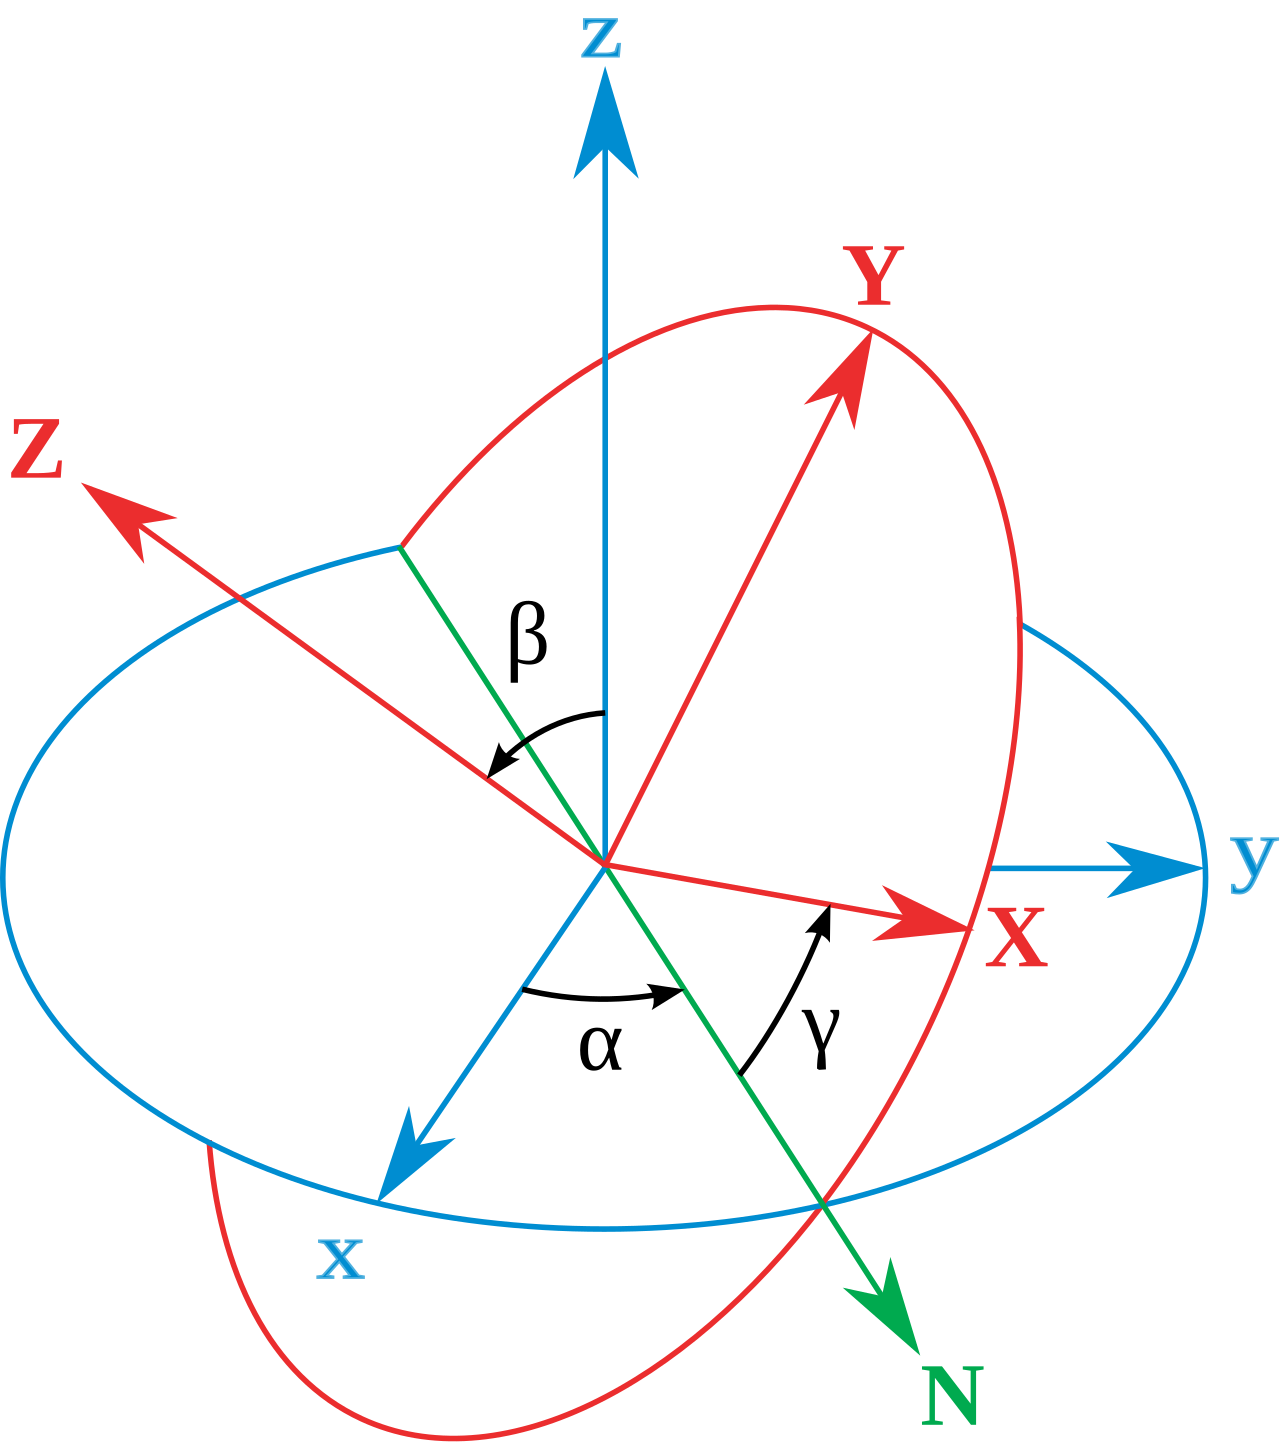
\includegraphics[width=0.65\textwidth]{Images/agent/he_toa_do_drone.png}
    \caption[Hệ tọa độ vật thể Body Frame của Quadcopter]{\bfseries\fontsize{12pt}{0pt}\selectfont Hệ tọa độ vật thể Body Frame của Quadcopter}
    \label{fig:he_toa_do_drone}
\end{figure}

Nguyên lý cân bằng và di chuyển của Quadcopter cấu hình Quad-X dựa trên chiều quay đối xứng của 4 motor (Hình \ref{fig:chieu_quay_motor}):
\begin{itemize}
    \item \textbf{Động cơ quay nghịch CCW}: Động cơ M1 (trước - phải) và M3 (sau - trái).
    \item \textbf{Động cơ quay thuận CW}: Động cơ M2 (sau - phải) và M4 (trước - trái).
\end{itemize}

\begin{figure}[H]
    \centering
    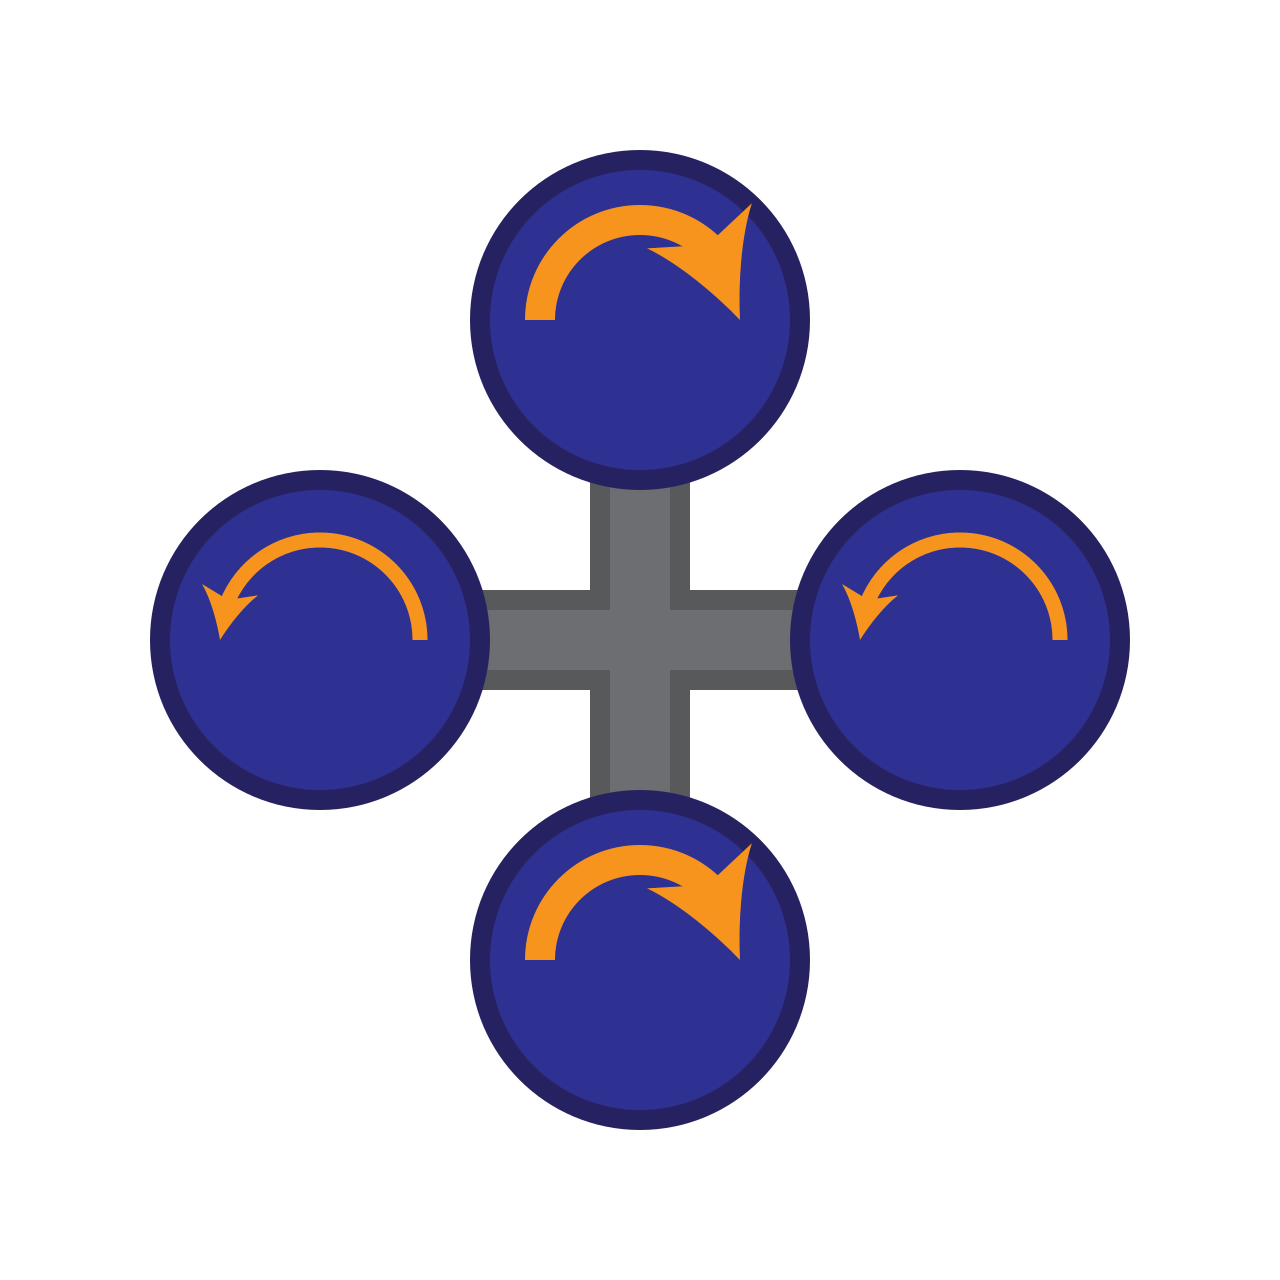
\includegraphics[width=0.65\textwidth]{Images/agent/chieu_quay_motor.png}
    \caption[Sơ đồ chiều quay động cơ cấu hình Quad-X]{\bfseries\fontsize{12pt}{0pt}\selectfont Sơ đồ chiều quay động cơ cấu hình Quad-X}
    \label{fig:chieu_quay_motor}
\end{figure}

Việc thay đổi tốc độ tương đối giữa các cặp động cơ tạo ra momen lực lệch thăng bằng để thực hiện các hành vi cơ động:
\begin{itemize}
    \item \textbf{Nghiêng phải (Roll dương)}: Tăng tốc các động cơ bên trái (M3, M4) và giảm tốc các động cơ bên phải (M1, M2).
    \item \textbf{Chúi mũi trước (Pitch âm)}: Tăng tốc các động cơ phía sau (M2, M3) và giảm tốc các động cơ phía trước (M1, M4).
    \item \textbf{Xoay trái CCW (Yaw dương)}: Tăng tốc các động cơ quay thuận CW (M2, M4) và giảm tốc các động cơ quay nghịch CCW (M1, M3). Mô-men phản lực lệch hướng sẽ làm thân drone xoay theo chiều ngược lại.
\end{itemize}

\subsection{Hệ thống điều khiển phản hồi PID vòng kín rời rạc}

Để duy trì sự cân bằng của Quadcopter trước các luồng gió nhiễu động từ môi trường bên ngoài, hệ thống nhúng liên tục chạy thuật toán điều khiển phản hồi PID vòng kín (Proportional-Integral-Derivative) trong miền rời rạc. Sơ đồ khối của bộ điều khiển được thể hiện trong Hình \ref{fig:so_do_khoi_pid}.

\begin{figure}[H]
    \centering
    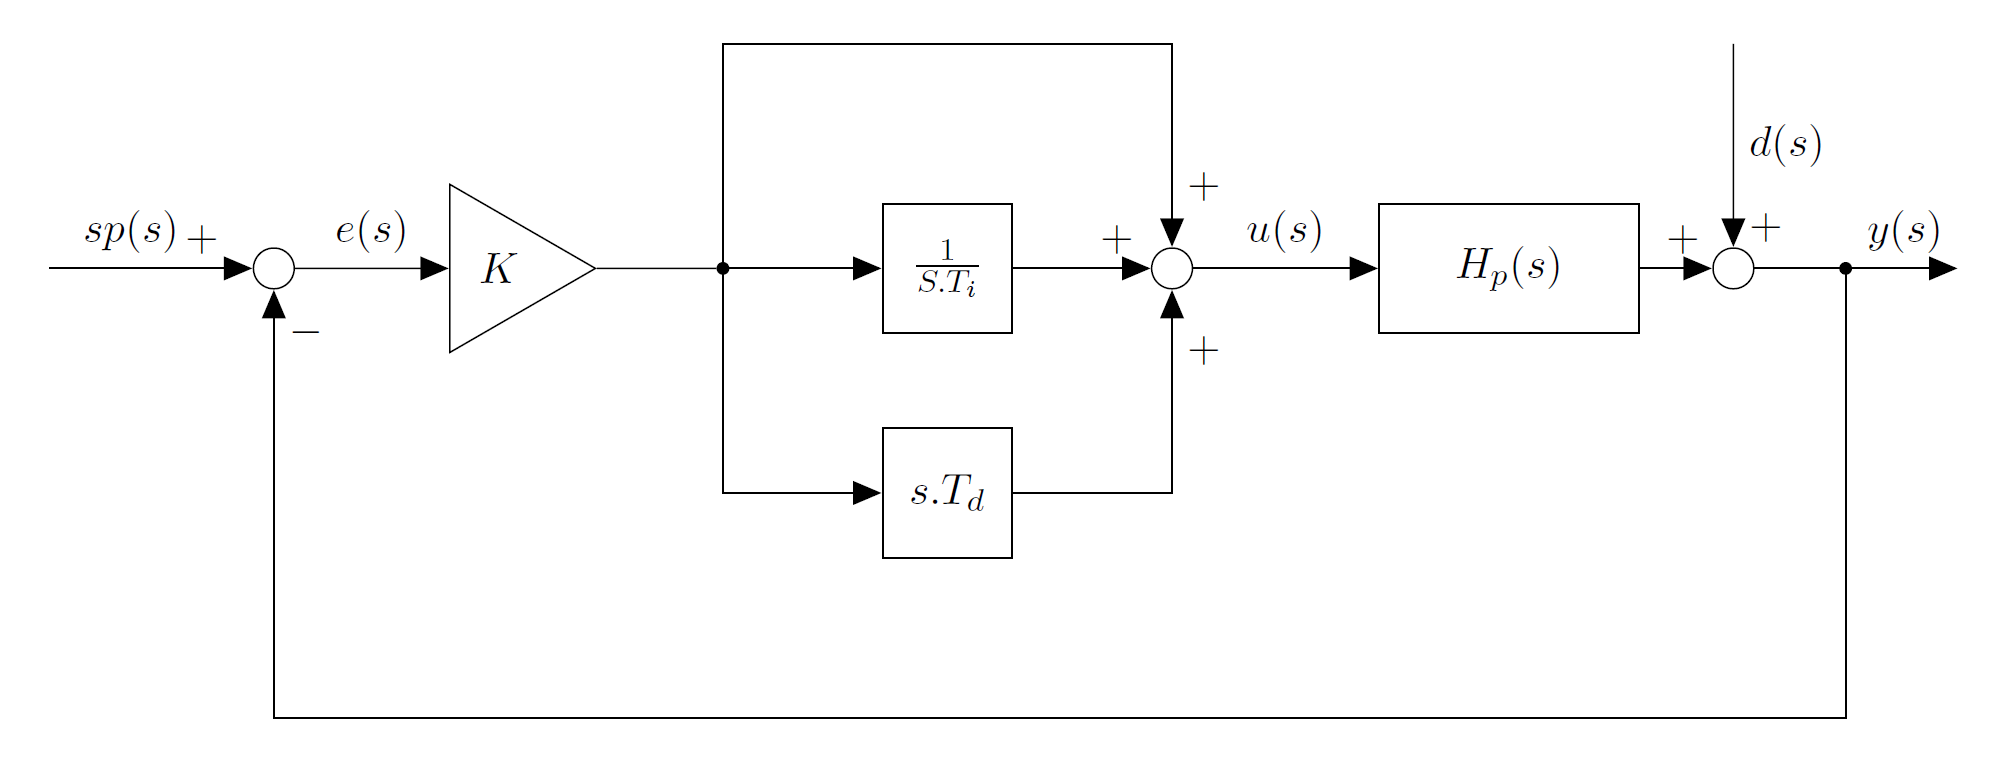
\includegraphics[width=0.85\textwidth]{Images/agent/so_do_khoi_pid.png}
    \caption[Sơ đồ khối bộ điều khiển phản hồi PID rời rạc]{\bfseries\fontsize{12pt}{0pt}\selectfont Sơ đồ khối bộ điều khiển phản hồi PID rời rạc}
    \label{fig:so_do_khoi_pid}
\end{figure}

Sai số góc nghiêng $e(t)$ tại thời điểm trích mẫu $n$ được định nghĩa bằng hiệu số giữa giá trị đặt từ tay điều khiển $Setpoint$ và góc nghiêng thực tế đo từ cảm biến $Feedback$:
\begin{equation}
    e[n] = Setpoint[n] - Feedback[n]
\end{equation}

Tín hiệu điều khiển đầu ra của khâu PID rời rạc được tính bằng công thức:
\begin{equation}
    u[n] = K_p \cdot e[n] + K_i \sum_{j=0}^{n} e[j] \cdot T + K_d \frac{e[n] - e[n-1]}{T}
\end{equation}
Trong đó, $T$ là chu kỳ trích mẫu của vòng điều khiển. Đối với hệ thống điều khiển nhúng Drone, hai hiện tượng kỹ thuật quan trọng cần được giải quyết triệt để trong firmware:

\begin{enumerate}
    \item \textbf{Hiện tượng bão hòa tích phân (Integral Windup)}: Xảy ra khi sai số lớn kéo dài khiến thành phần tích phân $I$ tăng quá mức giới hạn phần cứng của động cơ (vượt ngưỡng ga 2000$\mu s$). Khi Drone muốn đổi hướng gấp, khâu $I$ tích lũy quá lớn sẽ gây hiện tượng trễ đáp ứng nghiêm trọng, dẫn đến dao động quá đà hoặc lộn nhào (lật Drone). Thuật toán giải quyết bằng cơ chế **Anti-windup clamping** (khóa cứng giới hạn đầu ra khâu I ở mức $\pm 400$):
    \begin{equation}
        i\_mem = \max(\min(i\_mem + K_i \cdot e[n], PID\_MAX), -PID\_MAX)
    \end{equation}
    \item \textbf{Nhiễu khâu vi phân (Derivative Noise)}: Khâu vi phân cực kỳ nhạy cảm với các rung động cơ khí tần số cao của cánh quạt truyền qua khung sườn tới cảm biến IMU. Việc vi phân trực tiếp dữ liệu thô sẽ khuếch đại nhiễu làm nóng động cơ và gây cháy ESC. Hệ thống khắc phục bằng cách thiết lập **Bộ lọc thông thấp số IIR (Infinite Impulse Response)** bậc 1:
    \begin{equation}
        gyro\_input[n] = gyro\_input[n-1] \cdot 0.7 + new\_reading \cdot 0.3
    \end{equation}
\end{enumerate}

\subsection{Hệ thống cảm biến định vị quán tính IMU MPU6050 và Bộ lọc bù}

Cảm biến IMU MPU6050 \cite{mpu6050} tích hợp bộ cảm biến gia tốc 3 trục (Accelerometer) và cảm biến vận tốc góc 3 trục (Gyroscope) như mô tả trong Hình \ref{fig:truc_mpu6050}.

\begin{figure}[H]
    \centering
    
\includegraphics[width=0.45\textwidth]{Images/agent/truc_mpu6050.png}
    \caption[Sơ đồ các trục cảm biến trên chip MPU6050]{\bfseries\fontsize{12pt}{0pt}\selectfont Sơ đồ các trục cảm biến trên chip MPU6050}
    \label{fig:truc_mpu6050}
\end{figure}

Nguyên lý tính toán góc nghiêng từ cảm biến IMU có các đặc điểm đối nghịch:
\begin{itemize}
    \item \textbf{Gyroscope}: Tính góc bằng cách tích phân vận tốc góc theo thời gian: $\theta_{gyro} = \theta + \omega \cdot dt$. Khâu này phản hồi rất nhanh trước các chuyển động động học đột ngột, nhưng tích lũy sai số theo thời gian tạo ra hiện tượng trôi góc (Drift) do nhiễu offset DC của cảm biến.
    \item \textbf{Accelerometer}: Tính góc bằng công thức lượng giác dựa trên véc-tơ gia tốc trọng trường $g$:
    \begin{equation}
        \theta_{accel} = \arctan2(a_y, a_z) \cdot \frac{180}{\pi}
    \end{equation}
    Gia tốc trọng trường là mốc quy chiếu tuyệt đối nên góc tính từ accelerometer không bị trôi theo thời gian, nhưng nó cực kỳ nhạy cảm với các lực gia tốc động học của Drone lúc di chuyển và rung động cơ khí, gây nhiễu tức thời lớn.
\end{itemize}

Để dung hợp ưu điểm của hai cảm biến, hệ thống triển khai bộ lọc bù rời rạc (Complementary Filter) \cite{mahony2008} như sơ đồ trong Hình \ref{fig:bo_loc_bu}.

\begin{figure}[H]
    \centering
    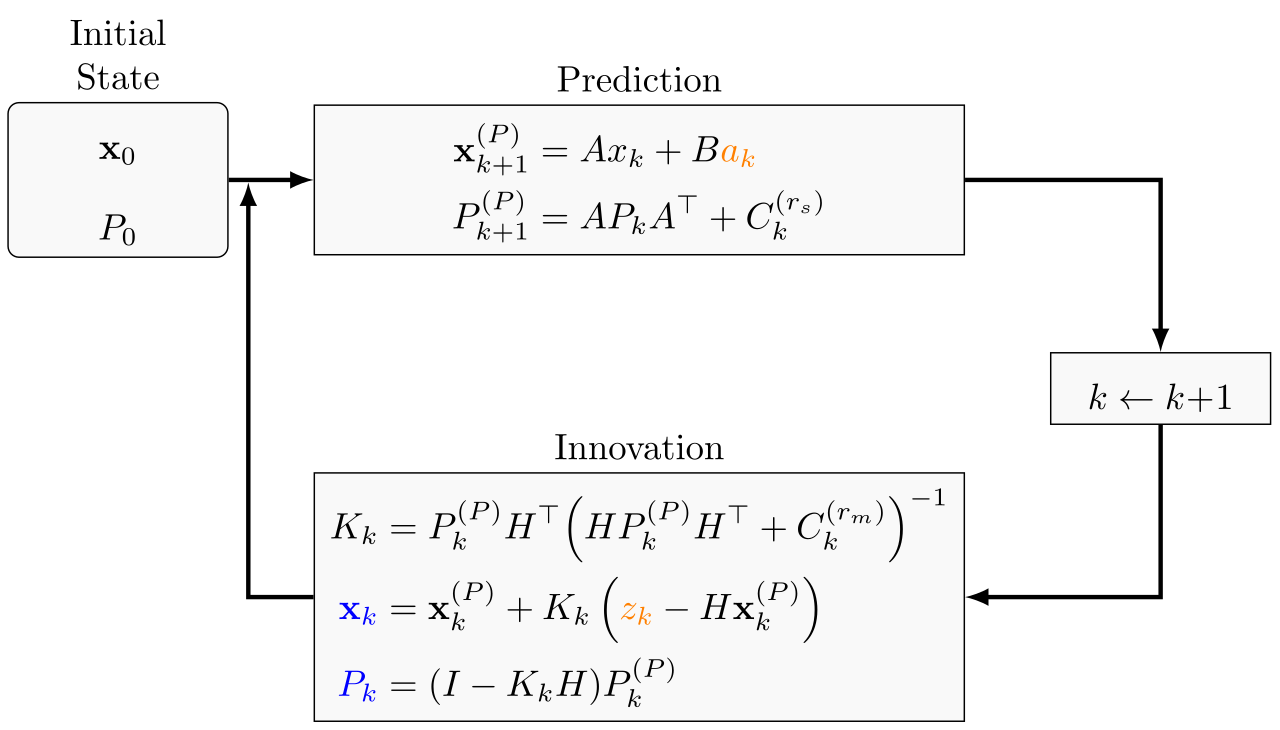
\includegraphics[width=0.8\textwidth]{Images/agent/bo_loc_bu.png}
    \caption[Sơ đồ thuật toán bộ lọc bù Complementary Filter]{\bfseries\fontsize{12pt}{0pt}\selectfont Sơ đồ thuật toán bộ lọc bù Complementary Filter}
    \label{fig:bo_loc_bu}
\end{figure}

Góc tư thế ước lượng tại mỗi chu kỳ trích mẫu được tính bằng công thức:
\begin{equation}
    \theta_{filter}[n] = \alpha \cdot (\theta_{filter}[n-1] + \omega_{gyro} \cdot dt) + (1 - \alpha) \cdot \theta_{accel}[n]
\end{equation}
Hệ số $\alpha$ được thiết lập bằng 0.98. Tỷ trọng này giúp hệ thống tin cậy 98\% vào sự thay đổi nhanh của Gyroscope trong thời gian ngắn, đồng thời liên tục lấy 2\% mốc tham chiếu tuyệt đối của Accelerometer để kéo góc lọc bù về giá trị thực, triệt tiêu hoàn toàn hiện tượng trôi góc.

\subsection{Giao thức truyền thông điều khiển vô tuyến CRSF và I2C}

ExpressLRS (ELRS) \cite{expresslrs2023} là công nghệ truyền sóng vô tuyến tầm xa mã nguồn mở hàng đầu hiện nay dựa trên công nghệ điều chế LoRa (Long Range), đem lại độ nhạy thu cực cao và khả năng xuyên nhiễu tuyệt đối. Bộ thu ELRS giao tiếp với Flight Controller thông qua giao thức truyền tin nối tiếp CRSF (Crossfire Protocol) với tốc độ baud rate tiêu chuẩn là 420.000\,bps.

Cấu trúc một khung dữ liệu CRSF được mô tả trực quan trong Hình \ref{fig:crsf_protocol}.

\begin{figure}[H]
    \centering
    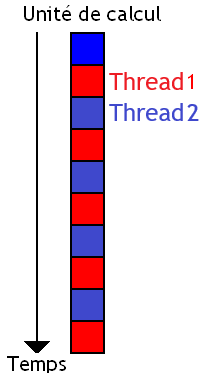
\includegraphics[width=0.85\textwidth]{Images/agent/crsf_protocol.png}
    \caption[Cấu trúc byte của khung dữ liệu giao thức CRSF]{\bfseries\fontsize{12pt}{0pt}\selectfont Cấu trúc byte của khung dữ liệu giao thức CRSF}
    \label{fig:crsf_protocol}
\end{figure}

Khung tin CRSF gồm các byte chức năng:
\begin{itemize}
    \item \textbf{Device Address (1 byte)}: Xác định đích đến (0xC8 cho Transmitter, 0xEE cho Flight Controller).
    \item \textbf{Frame Length (1 byte)}: Số lượng byte dữ liệu tiếp theo bao gồm cả byte CRC.
    \item \textbf{Type (1 byte)}: Định nghĩa loại dữ liệu (ví dụ 0x16 cho gói tin 16 kênh RC).
    \item \textbf{Payload (22 bytes)}: Chứa thông tin 16 kênh RC. Để tối ưu hóa băng thông, các kênh RC được đóng gói dưới dạng 11-bit trên mỗi kênh thay vì gửi 16-bit truyền thống.
    \item \textbf{CRC (1 byte)}: Mã kiểm tra lỗi CRC8 giúp loại bỏ hoàn toàn các khung tin bị sai lệch bit do nhiễu sóng.
\end{itemize}

Bên cạnh đó, việc lưu trữ các tham số cấu hình PID, căn chỉnh cảm biến được thực hiện qua bộ nhớ ROM EEPROM 24LC256 giao tiếp chuẩn I2C. Giản đồ xung timing của giao thức I2C được thể hiện trong Hình \ref{fig:i2c_timing}.

\begin{figure}[H]
    \centering
    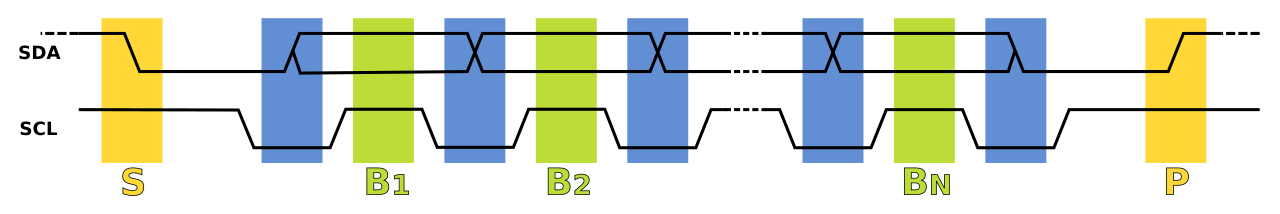
\includegraphics[width=0.85\textwidth]{Images/agent/i2c_timing.png}
    \caption[Giản đồ xung timing giao tiếp I2C giữa MCU và ngoại vi]{\bfseries\fontsize{12pt}{0pt}\selectfont Giản đồ xung timing giao tiếp I2C giữa MCU và ngoại vi}
    \label{fig:i2c_timing}
\end{figure}

Giao tiếp I2C sử dụng hai đường tín hiệu SCL (Serial Clock) và SDA (Serial Data). Cơ chế bao gồm xung START (SDA chuyển mức cao xuống thấp khi SCL cao), chuỗi bit dữ liệu đồng bộ theo nhịp clock SCL, bit ACK kiểm tra từ slave và xung STOP (SDA chuyển thấp lên cao khi SCL cao), giúp MCU ghi nhận cấu hình một cách chính xác tuyệt đối.


\bigskip
%%%% Phần 2.x+1--2.y: Thiết kế và chế tạo phần cứng %%%%
%%%%%%%%%%%%%%%%%%%%%%%%%%%%%%%%%%%%%%%%%%%%%%%%%%%
% CHƯƠNG 4: THIẾT KẾ VÀ CHẾ TẠO HỆ THỐNG PHẦN CỨNG DRONE VÀ TRẠM MẶT ĐẤT
%%%%%%%%%%%%%%%%%%%%%%%%%%%%%%%%%%%%%%%%%%%%%%%%%%%
\section*{CHƯƠNG 4. THIẾT KẾ VÀ CHẾ TẠO HỆ THỐNG PHẦN CỨNG DRONE VÀ TRẠM MẶT ĐẤT}
\addcontentsline{toc}{section}{\numberline{}CHƯƠNG 4. THIẾT KẾ VÀ CHẾ TẠO HỆ THỐNG PHẦN CỨNG DRONE VÀ TRẠM MẶT ĐẤT}
\setcounter{section}{4}
\setcounter{subsection}{0}
\setcounter{figure}{0}
\setcounter{table}{0}

\subsection{Thiết kế phần cứng và cơ khí Drone}

Việc tự thiết kế bo mạch điều khiển bay Flight Controller (FC) giúp nâng cao khả năng làm chủ công nghệ nhúng, tối ưu hóa kích thước và sơ đồ chân (pinout) theo đúng nhu cầu sử dụng thực tế của hệ thống Drone cứu nạn, đồng thời loại bỏ các tính năng dư thừa của các bo mạch thương mại.

Sơ đồ cấu trúc phần cứng tổng quát và các kết nối ngoại vi của toàn bộ hệ thống Drone được mô tả trong Hình \ref{fig:so_do_khoi_he_thong}.

\begin{figure}[H]
    \centering
    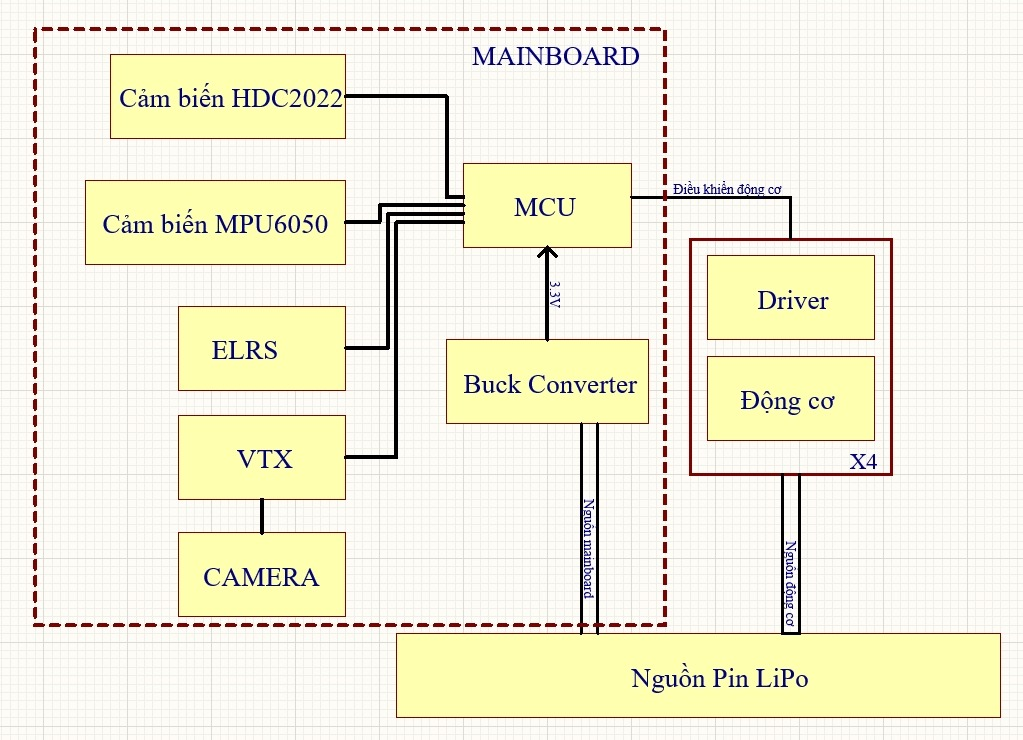
\includegraphics[width=0.85\textwidth]{Images/so_do_khoi_he_thong.jpg}
    \caption[Sơ đồ khối cấu trúc phần cứng và kết nối ngoại vi hệ thống Drone]{\bfseries\fontsize{12pt}{0pt}\selectfont Sơ đồ khối cấu trúc phần cứng và kết nối ngoại vi hệ thống Drone}
    \label{fig:so_do_khoi_he_thong}
\end{figure}

Hệ thống được chia làm hai khu vực chính:
\begin{itemize}
    \item \textbf{Bo mạch chính (Mainboard - Flight Controller):} Đóng vai trò là trung tâm xử lý dữ liệu và điều phối hoạt động bay. Tích hợp trên bo mạch bao gồm vi điều khiển (MCU) trung tâm kết nối trực tiếp với các cảm biến quán tính IMU MPU6050 (đọc vận tốc góc và gia tốc), cảm biến khí hậu HDC2022 (đo nhiệt độ và độ ẩm môi trường xung quanh), bộ thu sóng điều khiển ELRS (nhận lệnh từ tay phát) và bộ truyền hình ảnh VTX kết nối trực tiếp với camera FPV để truyền tải luồng video trực tuyến về trạm mặt đất. Một bộ hạ áp Buck Converter được tích hợp trực tiếp trên bo mạch để nhận điện áp cao từ pin LiPo và chuyển đổi thành nguồn sạch cấp cho MCU (qua bộ ổn áp LDO 3.3V) và các module cảm biến, thu phát sóng.
    \item \textbf{Hệ thống động lực ngoại vi:} Bao gồm bộ nguồn Pin LiPo dung lượng lớn để cung cấp năng lượng độc lập. Nguồn pin cấp trực tiếp cho 4 cụm Driver (ESC) và động cơ không chổi than, đồng thời dẫn tới ngõ vào nguồn của Mainboard. Vi điều khiển trung tâm (MCU) xuất 4 đường tín hiệu xung PWM chuyên dụng để điều khiển hoạt động đồng bộ của 4 động cơ thông qua các bộ ESC tương ứng.
\end{itemize}

\subsubsection{Thiết kế sơ đồ nguyên lý và Layout PCB Flight Controller}


Bo mạch điều khiển bay được thiết kế trên phần mềm Altium Designer xoay quanh vi điều khiển trung tâm STM32F103C8T6 (kiến trúc ARM Cortex-M3, hoạt động ở tần số 72\,MHz). Sơ đồ nguyên lý chi tiết được thiết kế chia làm hai bản vẽ chính:
\begin{itemize}
    \item \textbf{Bản vẽ nguồn chính và chuyển đổi nguồn (Hình \ref{fig:schematic_fc_power})}:
    \begin{itemize}
        \item \textit{Khối Power Main}: Sử dụng IC chuyển đổi nguồn dạng xung Buck TPS5450DDAR hiệu suất cao để chuyển đổi từ điện áp pin LiPo chính 12V xuống 5V. Đường vào được lọc nhiễu bởi tụ hóa C22 ($120\,\mu\text{F}/35\text{V}$) kết hợp tụ gốm C23 ($10\,\text{nF}$). Đầu ra sử dụng cuộn cảm L1 ($18\,\mu\text{H}$) kết hợp diode Schottky SS54 và các tụ lọc C26 ($220\,\mu\text{F}/10\text{V}$), C31 ($10\,\text{nF}$) để san phẳng điện áp ngõ ra 5V ổn định. Mạch phản hồi sử dụng cầu phân áp R5 ($18\,\text{k}\Omega$) và R10 ($5.6\,\text{k}\Omega$) để duy trì điện áp 5V chuẩn xác.
        \item \textit{Khối ổn áp tuyến tính 5V - 3.3V MCU}: Sử dụng IC AMS1117-3.3V để chuyển đổi từ nguồn 5V ổn định xuống 3.3V cấp cho vi điều khiển STM32 và các linh kiện logic nhạy cảm. Hệ thống tụ lọc đầu vào C27 ($22\,\mu\text{F}$), C28 ($100\,\text{nF}$) và đầu ra C29 ($100\,\text{nF}$), C30 ($22\,\mu\text{F}$) đảm bảo giảm thiểu tối đa nhiễu gợn sóng cao tần. LED D1 báo nguồn qua trở hạn dòng R9 ($1\,\text{k}\Omega$).
        \item \textit{Jack nguồn vào J2}: Sử dụng giắc DC5525 để nhận nguồn DC 12V từ pin 3S.
    \end{itemize}
    \item \textbf{Bản vẽ khối điều khiển và giao tiếp ngoại vi (Hình \ref{fig:schematic_fc_mcu})}:
    \begin{itemize}
        \item \textit{Khối MCU trung tâm}: Vi điều khiển STM32F103C8T6 với mạch Reset cứng (nút nhấn RST, trở kéo lên 10\,k$\Omega$, tụ lọc nhiễu 0.1\,$\mu$F), mạch dao động thạch anh ngoài 8\,MHz (CLOCK) sử dụng tụ lọc 22\,pF và mạch thạch anh thời gian thực 32.768\,kHz sử dụng tụ lọc 10\,pF.
        \item \textit{Khối cảm biến IMU MPU-6050}: Giao tiếp với MCU qua bus I2C (SCL, SDA) tích hợp các tụ lọc nguồn nhiễu C12, C13 (0.1\,$\mu$F).
        \item \textit{Khối bộ nhớ EEPROM 24LC256}: Lưu trữ các thông số hiệu chuẩn cảm biến và hệ số PID, kết nối qua bus I2C dùng chung với MPU-6050.
        \item \textit{Khối đo năng lượng (ĐO NL)}: Thiết kế mạch cầu phân áp gồm R8 ($27\,\text{k}\Omega$) và R12 ($10\,\text{k}\Omega$) để đo điện áp pin VBAT đưa về chân ADC của MCU.
        \item \textit{Khối kết nối ngoại vi}: Các giắc kết nối giao tiếp với mạch thu ELRS, mạch phát truyền hình ảnh VTX, và khối cảm biến khí tượng (AIR SENS) sử dụng cảm biến nhiệt độ - độ ẩm HDC2022DEPR qua I2C.
        \item \textit{Khối điều khiển động cơ (DRIVE A2212)}: Trích xuất các cổng PWM1 đến PWM4 từ Timer của STM32 cấp cho ESC điều khiển động cơ.
    \end{itemize}
\end{itemize}

\begin{figure}[H]
    \centering
    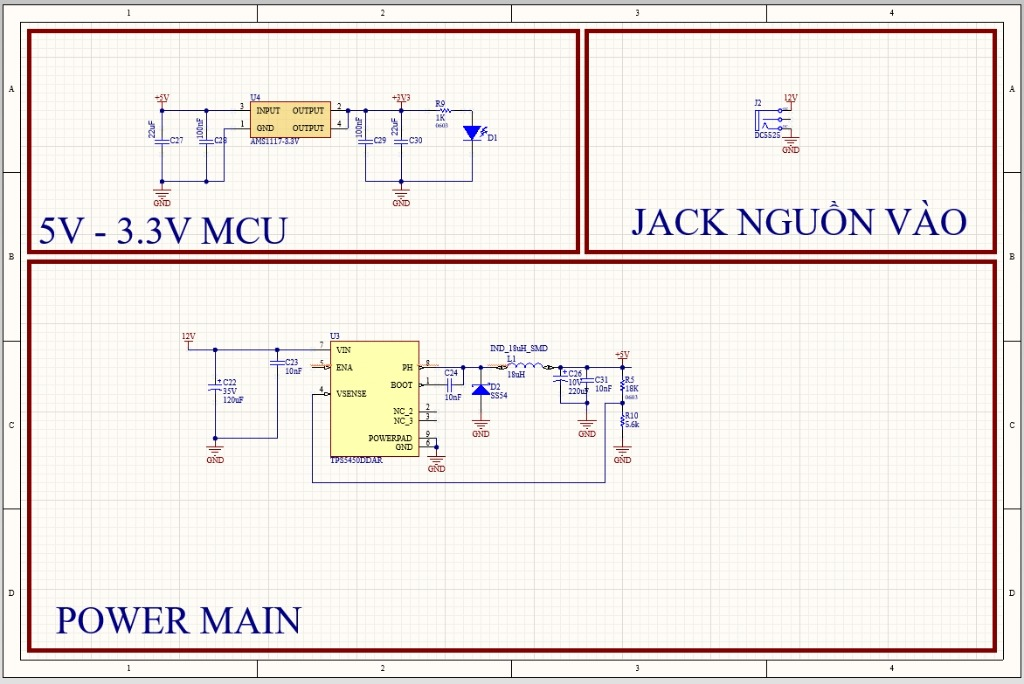
\includegraphics[width=0.95\textwidth]{Images/schematic_fc_power.jpg}
    \caption[Sơ đồ nguyên lý Flight Controller - Khối mạch nguồn chính]{\bfseries\fontsize{12pt}{0pt}\selectfont Sơ đồ nguyên lý Flight Controller - Khối mạch nguồn chính}
    \label{fig:schematic_fc_power}
\end{figure}

\begin{figure}[H]
    \centering
    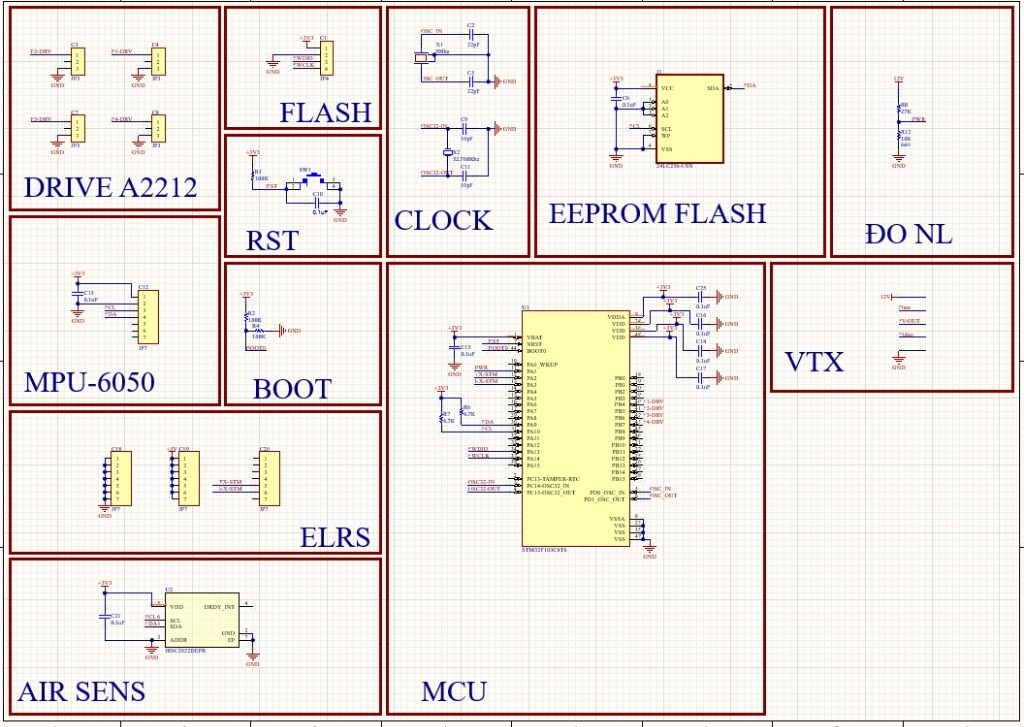
\includegraphics[width=0.95\textwidth]{Images/schematic_fc_mcu.jpg}
    \caption[Sơ đồ nguyên lý Flight Controller - Khối vi điều khiển và ngoại vi]{\bfseries\fontsize{12pt}{0pt}\selectfont Sơ đồ nguyên lý Flight Controller - Khối vi điều khiển và ngoại vi}
    \label{fig:schematic_fc_mcu}
\end{figure}

Layout PCB được thiết kế trên mạch 2 lớp (Double-sided PCB) với kích thước tiêu chuẩn 36\,x\,36\,mm, khoảng cách lỗ bắt ốc 30.5\,x\,30.5\,mm phù hợp với hầu hết các khung sườn Drone phổ thông. Chi tiết thiết kế Layout PCB và phối cảnh 3D của bo mạch Flight Controller được mô tả trong Hình \ref{fig:pcb_layout_3d}:
\begin{itemize}
    \item \textbf{Phối cảnh 3D}: Bo mạch được thiết kế dưới dạng hình bát giác đều cách điệu, bo tròn các góc để tăng tính cơ khí bền bỉ. Mạch khoét lỗ rỗng lớn ở tâm để tối ưu hóa việc phân bố trọng lượng, đi dây động lực xuyên qua sườn Drone và hỗ trợ tản nhiệt. Các linh kiện SMD được phân bố đồng đều, các cổng kết nối ngoại vi (như chân cắm nạp SWD, I2C, UART) được sắp xếp ở các mép cạnh giúp người vận hành dễ dàng thao tác cắm dây.
    \item \textbf{Lớp Top Layer (Mặt trên)}: Đi dây các đường nguồn chính với bề rộng lớn (VBAT, 5V, 3.3V) để tránh sụt áp và chịu tải dòng điện tốt. Các linh kiện công suất như IC TPS5450, cuộn cảm L1, tụ hóa C22 được ưu tiên đặt ở lớp trên. Các pad kết nối lớn ở viền mạch hỗ trợ cấp nguồn cho mạch truyền hình ảnh VTX và ESC.
    \item \textbf{Lớp Bottom Layer (Mặt dưới)}: Chứa các đường tín hiệu logic, I2C, UART kết nối chéo thông qua các lỗ via. Việc phân tách đường tín hiệu sang lớp Bottom giúp tránh hiện tượng nhiễu từ trường phát sinh từ các linh kiện công suất lớn ở lớp Top. Toàn bộ phần diện tích trống ở lớp dưới được phủ đồng GND để tối ưu khả năng khử nhiễu.
\end{itemize}

\begin{figure}[H]
    \centering
    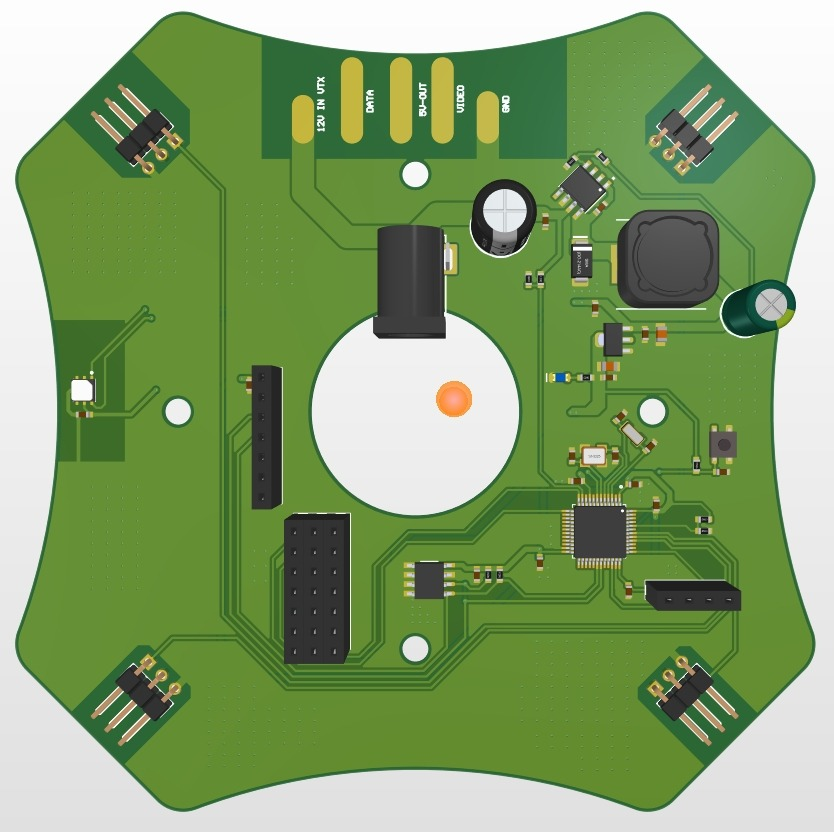
\includegraphics[width=0.31\textwidth]{Images/layout_pcb_fc_3d.jpg} \hfill
    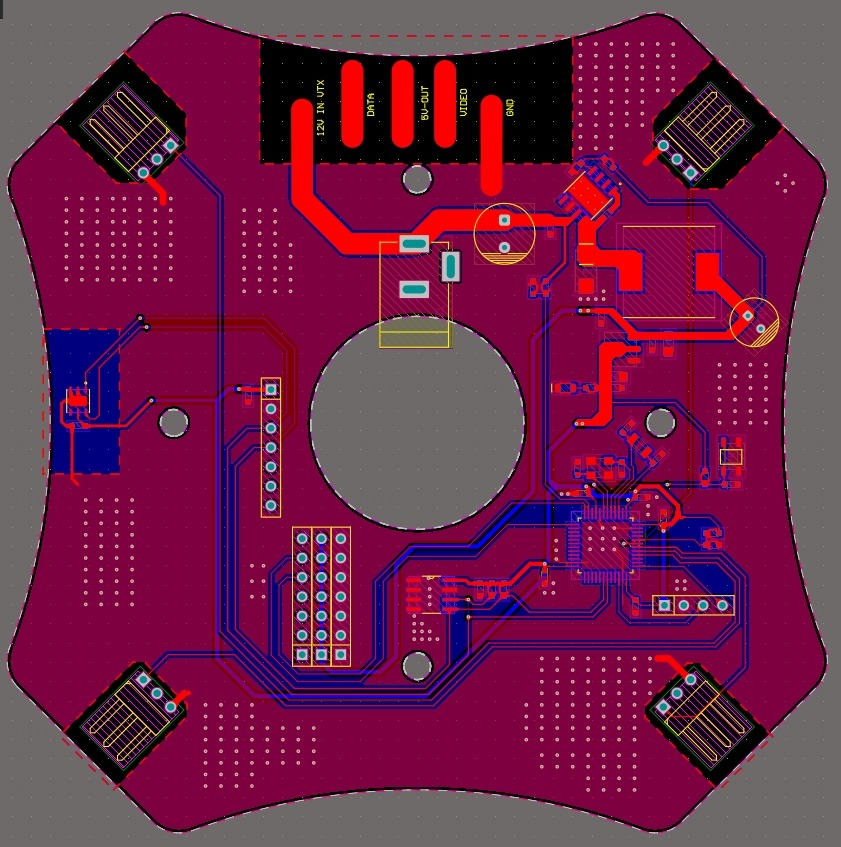
\includegraphics[width=0.31\textwidth]{Images/layout_pcb_fc_top.jpg} \hfill
    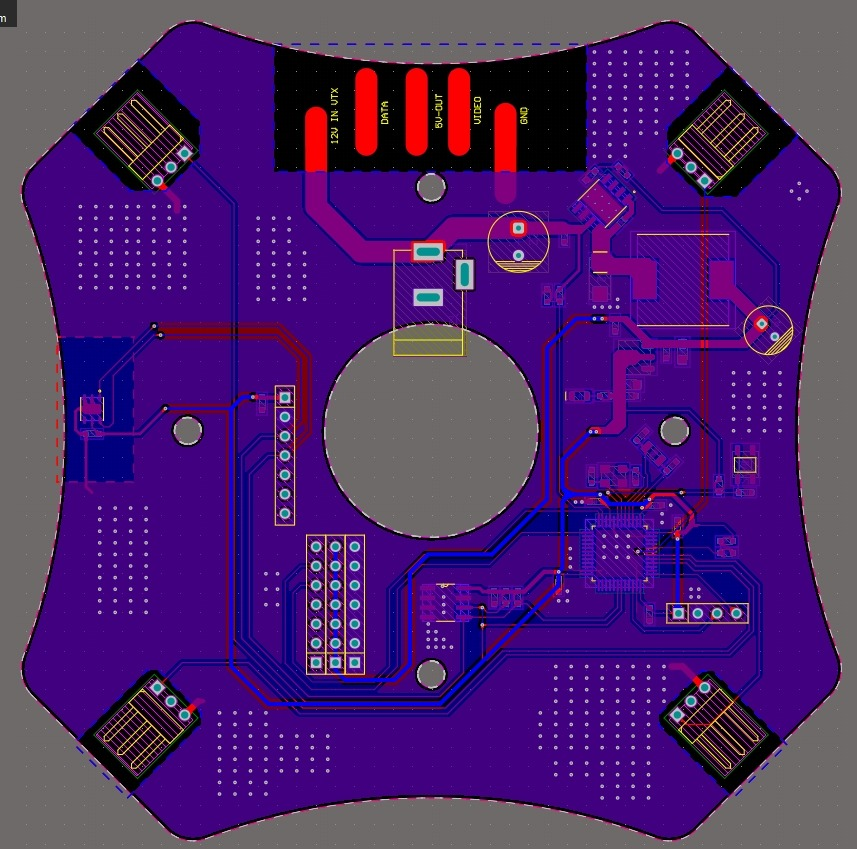
\includegraphics[width=0.31\textwidth]{Images/layout_pcb_fc_bottom.jpg}
    \caption[Thiết kế Layout PCB và phối cảnh 3D Flight Controller]{\bfseries\fontsize{12pt}{0pt}\selectfont Thiết kế Layout PCB và phối cảnh 3D Flight Controller: Phối cảnh 3D (trái), Layout lớp Top (giữa) và Layout lớp Bottom (phải)}
    \label{fig:pcb_layout_3d}
\end{figure}

\subsubsection{Thiết kế mạch nguồn logic và cầu phân áp đo pin}

Do các động cơ không chổi than khi thay đổi tốc độ đột ngột sẽ tạo ra các xung nhiễu điện áp ngược rất lớn trên đường nguồn chính VBAT, việc thiết kế hệ thống nguồn cấp điện cho các chip logic nhạy cảm (MCU, IMU) yêu cầu độ ổn định cực kỳ nghiêm ngặt. Sơ đồ mạch nguồn hạ áp phân tầng sử dụng chip nguồn xung Buck TPS5450DDAR kết hợp chip ổn áp tuyến tính LDO AMS1117-3.3V được thể hiện chi tiết tại Hình \ref{fig:schematic_fc_power}.

Hệ thống nguồn bao gồm hai tầng chính:
\begin{enumerate}
    \item \textbf{Tầng hạ áp Buck (TPS5450-5.0)}: Sử dụng IC hạ áp Buck chuyển mạch TPS5450DDAR của hãng Texas Instruments. Với tần số chuyển mạch cao 500\,kHz và dòng điện ngõ ra tối đa đạt 5A, TPS5450 cung cấp nguồn 5V mạnh mẽ và hiệu suất cao (>90\%) cho các tải lớn như bộ thu sóng ELRS, camera FPV, gimbal và cảm biến ngoại vi. Tụ hóa ngõ vào C22 ($120\,\mu\text{F}/35\text{V}$) triệt tiêu các xung áp sụt đột ngột, trong khi cuộn cảm L1 ($18\,\mu\text{H}$), diode SS54 và tụ hóa ngõ ra C26 ($220\,\mu\text{F}/10\text{V}$) tạo bộ lọc thông thấp làm mịn điện áp đầu ra.
    \item \textbf{Tầng ổn áp tuyến tính LDO (AMS1117-3.3)}: Ổn áp từ nguồn 5.0V trung gian xuống 3.3V cấp cho MCU STM32 và cảm biến MPU6050. Mạch LDO cung cấp điện áp cực kỳ sạch, triệt tiêu các nhiễu gợn sóng cao tần (high-frequency ripple) phát sinh từ mạch Buck.
\end{enumerate}

Để giám sát dung lượng pin nhằm đưa ra cảnh báo hạ cánh an toàn, một mạch cầu phân áp được thiết kế nối từ cực dương pin VBAT về chân ADC (PA4) của MCU:
\begin{equation}
    V_{ADC} = V_{BAT} \cdot \frac{R_2}{R_1 + R_2}
\end{equation}
Với giá trị điện trở lựa chọn $R_1 = 10\,k\Omega$ và $R_2 = 3.3\,k\Omega$, điện áp pin lớn nhất $12.6V$ được hạ xuống mức an toàn $3.12V$, nằm hoàn toàn trong dải đo tuyến tính của bộ ADC 12-bit trên vi điều khiển STM32 (0V - 3.3V).

\subsubsection{Lắp ráp cơ khí và hệ thống động lực}

Khung sườn Drone được sử dụng là khung Carbon FPV F450 chịu lực tốt và trọng lượng nhẹ. Hệ thống động lực được lựa chọn dựa trên sự tính toán cân bằng lực đẩy tối ưu:
\begin{itemize}
    \item \textbf{Động cơ}: A2212 1000KV không chổi than, cung cấp lực đẩy tối đa khoảng 850g mỗi động cơ ở mức ga 100\% khi đi kèm cánh quạt 1045. Tổng lực đẩy tối đa của 4 động cơ đạt 3400g.
    \item \textbf{Trọng lượng Drone}: Tổng trọng lượng cất cánh (bao gồm pin Lipo, camera FPV, mạch FC và khung sườn) là 950g. Tỷ số lực đẩy trên trọng lượng (Thrust-to-Weight Ratio) đạt:
    \begin{equation}
        \text{Tỷ lệ Lực đẩy/Trọng lượng} = \frac{3400g}{950g} \approx 3.58
    \end{equation}
    Tỉ số này lớn hơn ngưỡng an toàn tối thiểu 2.0 rất nhiều, đảm bảo Drone có khả năng gia tốc cực tốt, kháng gió mạnh và hoạt động ổn định ở môi trường ngoài trời.
    \item \textbf{Pin nguồn}: Pin LiPo 3S 11.1V 2200mAh dòng xả 45C cho phép cung cấp dòng điện liên tục lên tới $2.2 \times 45 = 99A$, đáp ứng hoàn hảo nhu cầu dòng điện tức thời cực đại khi cả 4 ESC hoạt động hết công suất.
\end{itemize}

Hình dạng thực tế của mô hình Drone sau khi lắp ráp cơ khí hoàn chỉnh và tích hợp bo mạch điều khiển bay Flight Controller được thể hiện trong Hình \ref{fig:drone_lap_rap_thuc_te}.

\begin{figure}[H]
    \centering
    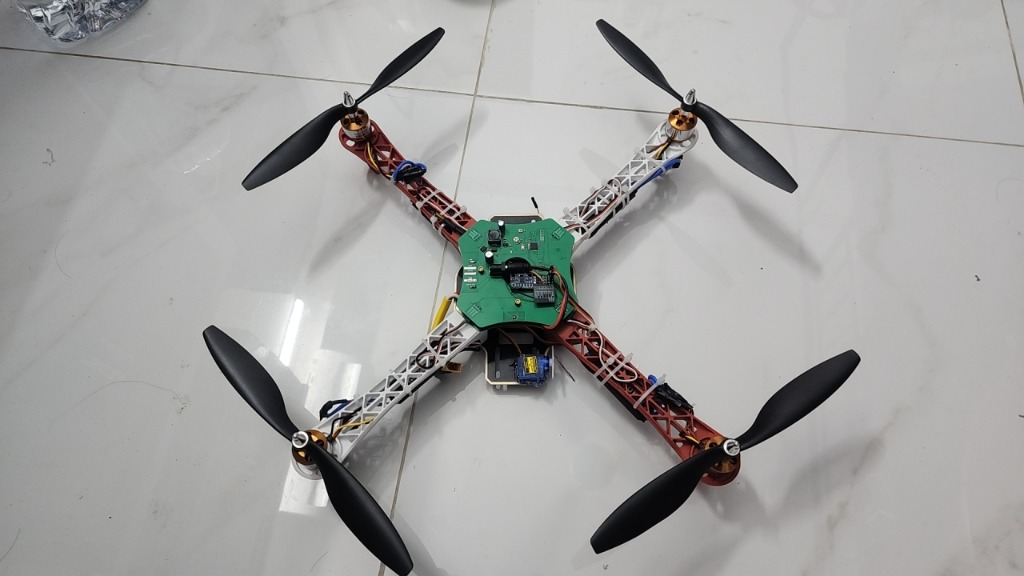
\includegraphics[width=0.65\textwidth]{Images/agent/drone_thuc_te.jpg}
    \caption[Mô hình thực tế hệ thống Drone cứu hộ hoàn thiện]{\bfseries\fontsize{12pt}{0pt}\selectfont Mô hình thực tế hệ thống Drone cứu hộ hoàn thiện}
    \label{fig:drone_lap_rap_thuc_te}
\end{figure}

\subsection{Lập trình phần mềm nhúng (Firmware Flight Controller)}

Firmware điều khiển bay được lập trình bằng ngôn ngữ C++ trực tiếp trên nền tảng Bare-metal (không sử dụng hệ điều hành thời gian thực RTOS) để tối ưu hóa tốc độ thực thi và loại bỏ độ trễ do chuyển đổi ngữ cảnh tác vụ (task context switching), đồng thời có tham khảo cơ chế lập lịch vòng lặp từ dự án mã nguồn mở Betaflight \cite{betaflight2024}.

\subsubsection{Kiến trúc vòng lặp điều khiển chính thời gian thực tần số 250Hz}

Độ ổn định của thiết bị bay phụ thuộc quyết định vào tính ổn định thời gian thực của vòng lặp điều khiển chính. Chu kỳ vòng lặp được thiết lập cố định ở tần số 250\,Hz (tương đương chu kỳ lấy mẫu $T_s = 4000\mu s$). Lưu đồ thuật toán khởi động và trạng thái của máy trạng thái (FSM) trong firmware được trình bày trong Hình \ref{fig:luu_do_fsm_boot}.

\begin{figure}[H]
    \centering
    \resizebox{0.85\textwidth}{!}{
    \begin{tikzpicture}[
        arrow/.style={-Latex, thick, draw=black},
        state/.style={rectangle, draw=black, fill=white, thick, minimum width=5.2cm, minimum height=1.0cm, align=center, rounded corners=3pt, font=\fontsize{8.5pt}{10pt}\selectfont},
        errorstate/.style={rectangle, draw=black, fill=gray!10, thick, minimum width=5.0cm, minimum height=1.2cm, align=center, rounded corners=3pt, font=\fontsize{8.5pt}{10pt}\selectfont}
    ]
        % Entry Point
        \node[circle, fill=black, inner sep=2.5pt, label=above:{\fontsize{8.5pt}{10pt}\selectfont Khởi động hệ thống (Power On)}] (start) at (0, 5.8) {};

        % States (Main path)
        \node[state] (boot) at (0, 4.6) {\textbf{STARTUP\_BOOT}\\Tải cấu hình từ lưu trữ};
        \node[state] (imu_init) at (0, 3.0) {\textbf{STARTUP\_IMU\_INIT}\\Khởi tạo cảm biến MPU6050};
        \node[state] (gyro_calib) at (0, 1.4) {\textbf{STARTUP\_GYRO\_CALIB}\\Hiệu chuẩn Gyroscope (1000 mẫu)};
        \node[state] (rc_check) at (0, -0.2) {\textbf{STARTUP\_RC\_CHECK}\\Kiểm tra kết nối và tay ga RC};
        \node[state] (acc_check) at (0, -1.8) {\textbf{STARTUP\_ACC\_CHECK}\\Kiểm tra gia tốc tĩnh ($g \approx 1.0$)};
        \node[state] (esc_check) at (0, -3.4) {\textbf{STARTUP\_ESC\_CHECK}\\Kiểm tra cờ calib ESC/Accel};
        \node[state, fill=gray!2] (ready) at (0, -5.0) {\textbf{STARTUP\_READY}\\Sẵn sàng bay (Vòng lặp chính)};

        % Error State
        \node[errorstate] (error) at (9.5, -1.0) {\textbf{STARTUP\_ERROR}\\Dừng động cơ khẩn cấp\\(Nháy chớp LED báo lỗi)};

        % Transitions (Main path)
        \draw[arrow] (start) -- (boot.north);
        \draw[arrow] (boot.south) -- (imu_init.north);
        
        \draw[arrow] (imu_init.south) -- node[right, font=\fontsize{7.5pt}{7.5pt}\selectfont] {Thành công} (gyro_calib.north);
        
        \draw[arrow] (gyro_calib.south) -- node[right, font=\fontsize{7.5pt}{7.5pt}\selectfont] {Thành công} (rc_check.north);
        
        \draw[arrow] (rc_check.south) -- node[right, font=\fontsize{7.5pt}{7.5pt}\selectfont] {Thành công} (acc_check.north);
        
        \draw[arrow] (acc_check.south) -- node[right, font=\fontsize{7.5pt}{7.5pt}\selectfont] {Thành công} (esc_check.north);
        
        \draw[arrow] (esc_check.south) -- node[right, font=\fontsize{7.5pt}{7.5pt}\selectfont] {Hoàn thành} (ready.north);

        % Gyro Self-loop
        \draw[arrow] (gyro_calib.west) .. controls ++(-1.6, 0.4) and ++(-1.6, -0.4) .. (gyro_calib.west) 
            node[pos=0.5, left, font=\fontsize{7.5pt}{7.5pt}\selectfont, align=center] {Phát hiện rung lắc\\(Thử lại $<$ 5 lần)};

        % Coordinates for error anchors
        \coordinate (err_1) at ([yshift=0.4cm]error.west);
        \coordinate (err_2) at ([yshift=0.15cm]error.west);
        \coordinate (err_3) at ([yshift=-0.1cm]error.west);
        \coordinate (err_4) at ([yshift=-0.35cm]error.west);

        % Error Transitions (using explicit segments)
        \draw[arrow] (imu_init.east) -- (6.7, 3.0) -- (6.7, -0.6) -- (err_1);
        \draw[arrow] (gyro_calib.east) -- (6.5, 1.4) -- (6.5, -0.85) -- (err_2);
        \draw[arrow] (rc_check.east) -- (6.3, -0.2) -- (6.3, -1.1) -- (err_3);
        \draw[arrow] (acc_check.east) -- (6.5, -1.8) -- (6.5, -1.35) -- (err_4);

        % Labels for error transitions (placed to the left of the vertical lines)
        \node[above right, font=\fontsize{7.5pt}{7.5pt}\selectfont, align=left, inner sep=2pt] at (imu_init.east) {Lỗi kết nối I2C\\(ERR\_IMU\_INIT\_FAIL)};
        \node[above right, font=\fontsize{7.5pt}{7.5pt}\selectfont, align=left, inner sep=2pt] at (gyro_calib.east) {Rung lắc quá 5 lần\\(ERR\_GYRO\_CALIB\_MOVING)};
        \node[above right, font=\fontsize{7.5pt}{7.5pt}\selectfont, align=left, inner sep=2pt] at (rc_check.east) {Mất sóng/Ga cao/Lệch cần\\(ERR\_RC\_CENTER / ERR\_THROTTLE)};
        \node[above right, font=\fontsize{7.5pt}{7.5pt}\selectfont, align=left, inner sep=2pt] at (acc_check.east) {Lệch trục gia tốc tĩnh\\(ERR\_ACC\_VALIDATION\_FAIL)};

        % CLI Command Reset
        \draw[arrow] (error.east) -- (13.0, -1.0) -- (13.0, 4.6) -- (boot.east)
            node[pos=0.25, right, font=\fontsize{7.5pt}{7.5pt}\selectfont, align=left] {Nhận lệnh 'c' qua CLI\\(Reset trạng thái lỗi)};

    \end{tikzpicture}
    }
    \caption[Sơ đồ máy trạng thái khởi động FSM Boot của Drone]{Sơ đồ máy trạng thái khởi động FSM Boot của Drone}
    \label{fig:luu_do_fsm_boot}
\end{figure}

Quy trình hoạt động trong vòng lặp chính của firmware bao gồm các bước tuần tự được đồng bộ thời gian khắt khe:
\begin{enumerate}
    \item \textbf{Chờ đồng bộ}: Sử dụng bộ đếm thời gian hệ thống High-Resolution Microsecond Timer để đo đạc chính xác thời điểm bắt đầu vòng lặp mới, đảm bảo đúng chu kỳ $4000\mu s$.
    \item \textbf{Đọc dữ liệu IMU}: Giao tiếp bus I2C đọc các thanh ghi dữ liệu thô của Gyroscope và Accelerometer trên MPU6050.
    \item \textbf{Ước lượng tư thế}: Thực thi thuật toán bộ lọc bù để tính toán góc nghiêng hiện tại (Roll, Pitch, Yaw).
    \item \textbf{Giải mã lệnh điều khiển}: Đọc luồng dữ liệu CRSF từ bộ thu sóng để cập nhật giá trị Setpoint mong muốn của người điều khiển.
    \item \textbf{Tính toán PID song song}: Chạy đồng thời 3 bộ điều khiển PID kép (Cascade PID) cho 3 trục bay để tính toán giá trị hiệu chỉnh lực nâng.
    \item \textbf{Trộn ga và xuất xung PWM}: Trộn giá trị điều khiển PID với tay ga chính (Throttle) để tính toán chu kỳ nhiệm vụ PWM cấp cho từng động cơ theo cấu hình Quad-X.
\end{enumerate}

\subsubsection{Giao tiếp Software I2C tốc độ cao và Đọc/Ghi EEPROM}

Do cảm biến MPU6050 và EEPROM 24LC256 nằm chung trên bus I2C, việc quản lý truyền thông không được để xảy ra hiện tượng nghẽn bus làm gián đoạn vòng lặp 250\,Hz. Đồ án xây dựng driver Software I2C (Bit-banging) sử dụng trực tiếp các thanh ghi cấu hình IO tốc độ cao của STM32 để đạt tần số clock truyền thông lên tới 400\,kHz (Fast Mode).

Bộ nhớ EEPROM 24LC256 được phân vùng để lưu trữ:
\begin{itemize}
    \item Giá trị hiệu chuẩn điểm không cảm biến (Gyro Offset, Accel Calibration).
    \item Các hệ số điều khiển PID ($K_p, K_i, K_d$) của 3 trục Roll, Pitch, Yaw.
\end{itemize}
Khi cấp nguồn, MCU sẽ đọc cấu hình từ EEPROM để khởi tạo hệ thống. Khi người dùng thay đổi PID từ trạm mặt đất, các tham số mới sẽ được ghi đè vào EEPROM một cách an toàn.

\subsubsection{Giải mã CRSF và Cơ chế an toàn Failsafe}

Giao thức CRSF từ bộ thu ELRS truyền về MCU qua cổng UART dưới dạng các khung tin nhị phân. Firmware sử dụng kỹ thuật ngắt nhận dữ liệu UART kết hợp bộ đệm vòng (Ring Buffer) để tránh làm mất mát dữ liệu khi MCU đang bận tính toán PID.

Mỗi khung dữ liệu nhận được chứa 11-bit giá trị tay ga cho mỗi kênh (từ 172 đến 1811, tương ứng thời gian xung từ $988\mu s$ đến $2012\mu s$). Hàm giải mã trích xuất kênh điều khiển và thực hiện chuyển đổi tuyến tính sang góc đặt Setpoint nghiêng từ $-30^\circ$ đến $+30^\circ$.

Để đảm bảo an toàn tuyệt đối cho người vận hành và thiết bị bay, cơ chế an toàn **Failsafe** được xây dựng chặt chẽ:
\begin{itemize}
    \item Firmware liên tục giám sát khoảng thời gian nhận được gói tin CRSF thành công gần nhất.
    \item Nếu quá thời gian $T_{lost} = 500\mu s$ mà không nhận được tín hiệu điều khiển mới từ bộ thu (mất sóng, hết pin tay phát), hệ thống sẽ tự động kích hoạt chế độ Failsafe: ngắt kích hoạt động cơ ngay lập tức (Disarm) để tránh hiện tượng Drone tự bay mất kiểm soát (Fly-away).
\end{itemize}

\subsection{Thiết kế phần mềm điều phối trạm mặt đất}

Phần mềm trạm mặt đất (GCS) được phát triển bằng ngôn ngữ Python sử dụng thư viện giao diện đồ họa PyQt5, đóng vai trò nhận luồng video thời gian thực từ đầu thu FPV, chạy các mô hình AI phát hiện sự kiện cứu hộ và tương tác với người vận hành.

\subsubsection{Kiến trúc hệ thống điều phối đa luồng (Multi-threading)}

Để đảm bảo giao diện đồ họa GUI hoạt động mượt mà và không bị giật lag khi đang thực hiện các phép toán nhận diện học sâu cực kỳ nặng, kiến trúc phần mềm được thiết kế phân lớp đa luồng như mô tả trong Hình \ref{fig:luong_phan_mem_gui}.

\begin{figure}[H]
    \centering
    \begin{tikzpicture}[
        node distance=1.2cm and 1.2cm,
        thread/.style={rectangle, draw=black, fill=white, thick, rounded corners, minimum width=3.4cm, minimum height=1.1cm, align=center, font=\bfseries\fontsize{9pt}{11pt}\selectfont},
        data/.style={ellipse, draw=black, fill=white, thick, minimum width=2.4cm, minimum height=0.9cm, align=center, font=\fontsize{8pt}{9pt}\selectfont},
        queue/.style={rectangle, draw=black, fill=white, thick, minimum width=2.6cm, minimum height=0.9cm, align=center, font=\fontsize{8pt}{9pt}\selectfont},
        io/.style={rectangle, draw=black, fill=white, thick, rounded corners=2pt, minimum width=2.4cm, minimum height=0.9cm, align=center, font=\fontsize{8pt}{9pt}\selectfont},
        arrow/.style={-Latex, thick, draw=black},
        signal/.style={-Latex, dashed, thick, draw=black, text=black, font=\fontsize{7.5pt}{8.5pt}\selectfont}
    ]

        % Grid Layout Configuration (Monochrome)
        % Column 1: x = 0
        % Column 2: x = 4.2
        % Column 3: x = 8.4
        % Column 4: x = 12.6
        
        % Row 1: y = 3
        \node[io] (camera) at (0,3) {Camera FPV\\(Dữ liệu video thô)};
        \node[thread] (video_thread) at (4.2,3) {Luồng nhận video\\(Sử dụng OpenCV)};
        \node[queue] (frame_queue) at (8.4,3) {Hàng đợi khung hình\\(Thread-safe Queue)};
        \node[thread] (inference_thread) at (12.6,3) {Luồng suy luận AI\\(YOLOv8 \& Dung hợp)};
        
        % Row 2: y = 0
        \node[io] (serial_port) at (0,0) {Bộ thu ELRS\\(Kết nối UART / USB)};
        \node[thread] (serial_thread) at (4.2,0) {Luồng nhận Telemetry\\(Giải mã dữ liệu Serial)};
        \node[thread] (gui_thread) at (8.4,0) {Luồng giao diện GUI\\(Luồng chính PyQt5)};
        \node[data] (target_mgr) at (12.6,0) {Bộ quản lý mục tiêu\\\& Khóa bám};
        
        % Row 3: y = -2
        \node[io] (operator) at (8.4,-2) {Màn hình trạm GCS\\(Giám sát \& Điều khiển)};

        % Connectors
        \draw[arrow] (camera) -- (video_thread);
        \draw[arrow] (video_thread) -- node[above, font=\fontsize{8pt}{9pt}\selectfont] {30 FPS} (frame_queue);
        \draw[arrow] (frame_queue) -- (inference_thread);
        
        \draw[arrow] (serial_port) -- (serial_thread);
        
        % Signals to GUI Thread (Rerouted with explicit label nodes to guarantee no overlap)
        \draw[signal] (inference_thread.south) -- ++(0,-0.25) -| ($(gui_thread.north east)-(0.4,0)$);
        \node[align=center, font=\fontsize{7.5pt}{8.5pt}\selectfont] at (10.7, 1.75) {Tín hiệu PyQt\\(Khung hình, Khung xương,\\Danger Score)};
            
        \draw[signal] (serial_thread.north) -- ++(0,0.25) -| ($(gui_thread.north west)+(0.4,0)$);
        \node[align=center, font=\fontsize{7.5pt}{8.5pt}\selectfont] at (5.8, 1.25) {Tín hiệu PyQt\\(Góc nghiêng,\\Điện áp pin)};
        
        \draw[arrow] (gui_thread) -- (operator);
        
        % Target Manager bidirectional connection
        \draw[arrow] ($(gui_thread.east)+(0,0.15)$) -- ($(target_mgr.west)+(0,0.15)$);
        \draw[arrow] ($(target_mgr.west)-(0,0.15)$) -- ($(gui_thread.east)-(0,0.15)$);

    \end{tikzpicture}
    \caption[Sơ đồ kiến trúc xử lý đa luồng tại trạm mặt đất GCS]{\bfseries\fontsize{12pt}{0pt}\selectfont Sơ đồ kiến trúc xử lý đa luồng tại trạm mặt đất GCS}
    \label{fig:luong_phan_mem_gui}
\end{figure}

Các luồng xử lý chạy song song độc lập tương tác qua cơ chế tín hiệu (Signals/Slots):
\begin{enumerate}
    \item \textbf{Luồng chính (GUI Thread)}: Đảm nhận việc vẽ giao diện người dùng, hiển thị khung hình video và tương tác nút nhấn.
    \item \textbf{Luồng nhận dữ liệu video (Video Ingestion Thread)}: Kết nối với camera FPV hoặc card capture USB để bắt các khung hình thô (raw frames) ở tốc độ 30 FPS bằng OpenCV, đẩy khung hình vào hàng đợi trung gian (Frame Queue).
    \item \textbf{Luồng suy luận AI (Inference Thread)}: Lấy khung hình từ Frame Queue, đẩy qua bộ Detector tích hợp 3 mô hình YOLO (YOLOv8-Rescue, YOLOv8-Posture, YOLOv8-Pose), thực hiện thuật toán dung hợp suy luận và gửi kết quả khung hình đã vẽ bounding box cùng tọa độ keypoints về GUI Thread.
    \item \textbf{Luồng Telemetry (Serial Communication Thread)}: Giao tiếp nối tiếp với mạch phát ELRS để nhận dữ liệu trạng thái Drone (điện áp pin, góc nghiêng thực tế) gửi ngược từ Drone về.
\end{enumerate}

\subsubsection{Bộ quản lý mục tiêu (Target Manager) và khóa mục tiêu (Focus Lock)}

Trong các tình huống giám sát đám đông hoặc khu vực thiên tai lớn, nhiều đối tượng có thể xuất hiện đồng thời trong một khung hình. Hệ thống xây dựng module **Target Manager** để theo dõi và quản lý định danh (ID) của từng mục tiêu:
\begin{itemize}
    \item Sử dụng thuật toán theo dõi đối tượng đa mục tiêu **ByteTrack** để gán ID duy nhất cho từng người phát hiện được dựa trên sự tương đồng về đặc trưng và khoảng cách giao nhau IoU (Intersection over Union) giữa các khung hình liên tiếp.
    \item Người vận hành có thể click chọn trực tiếp một mục tiêu cụ thể trên màn hình để kích hoạt cơ chế **Focus Lock** (Khóa nét tiêu điểm). Khi khóa nét, hệ thống sẽ tập trung tài nguyên tính toán để phân tích chi tiết tư thế keypoints và cử chỉ động cho duy nhất đối tượng đó, đồng thời gửi lệnh điều khiển gimbal camera quay bám đuổi mục tiêu được chọn.
\end{itemize}

\subsubsection{Giao diện tương tác và Hệ thống phím điều khiển của người vận hành}

Để đảm bảo khả năng phản ứng nhanh và linh hoạt của người vận hành trạm mặt đất trong các tình huống cứu nạn phức tạp, hệ thống thiết lập một giao diện tương tác tích hợp cho phép điều khiển và can thiệp trực tiếp bằng bàn phím và chuột. Các chức năng tương tác cốt lõi của người vận hành bao gồm:
\begin{itemize}
    \item \textbf{Phím quyết định của người vận hành (Operator Decisions)}:
    \begin{itemize}
        \item Phím \texttt{C} (Confirmed): Người vận hành chủ động xác nhận đối tượng đang khóa nét (Focus Target) thực sự là nạn nhân cần cứu trợ. Hành động này bỏ qua các đánh giá tự động và ngay lập tức lưu thông tin sự kiện kèm media.
        \item Phím \texttt{F} (False Alarm): Đánh dấu đối tượng được phát hiện là báo động giả. Hệ thống sẽ tự động hủy trạng thái nguy hiểm của đối tượng và xóa các file hình ảnh/video liên quan để giải phóng bộ nhớ.
        \item Phím \texttt{T} (Track More): Đánh dấu yêu cầu tiếp tục theo dõi tăng cường đối tượng này để thu thập thêm thông tin.
    \end{itemize}
    \item \textbf{Phím quản lý vùng giám sát nguy hiểm (ROI Controls)}:
    \begin{itemize}
        \item Phím \texttt{O}: Bật hoặc tắt tính năng giám sát vùng ROI.
        \item Phím \texttt{E}: Kích hoạt chế độ vẽ vùng nguy hiểm bằng cách click chuột để tạo các điểm đỉnh đa giác polygon trên màn hình.
        \item Phím \texttt{X}: Xóa bỏ hoàn toàn các cấu hình vùng ROI hiện tại.
    \end{itemize}
    \item \textbf{Phím thay đổi giao diện hiển thị (Display Controls)}:
    \begin{itemize}
        \item Giữ phím \texttt{Tab}: Hiển thị lớp phủ bảng thông số chấm điểm chi tiết (Overlay Panel) của mục tiêu đang chọn.
        \item Phím \texttt{P}: Bật hoặc tắt hiển thị khung xương 17 khớp (Skeleton).
        \item Phím \texttt{B}: Bật hoặc tắt thước ngắm chữ thập trung tâm (Crosshair) để hỗ trợ điều khiển camera bám đuổi.
    \end{itemize}
    \item \textbf{Phím điều phối hệ thống chung}:
    \begin{itemize}
        \item Phím \texttt{N}: Chuyển đổi khóa nét (Focus Lock) sang mục tiêu tiếp theo xuất hiện trong khung hình.
        \item Phím \texttt{S}: Khóa tiêu điểm nhanh vào đối tượng có Danger Score cao nhất.
        \item Phím \texttt{W}: Force refresh - yêu cầu cập nhật tức thời dữ liệu thời tiết tại trạm.
        \item Phím \texttt{A}: Mở cửa sổ Tkinter liệt kê danh sách nhật ký các sự kiện đã ghi nhận.
        \item Phím \texttt{R}: Xuất báo cáo HTML tức thời tại thời điểm hiện tại.
        \item Phím \texttt{Q} hoặc \texttt{Esc}: Lưu toàn bộ nhật ký sự kiện, tự động xuất báo cáo HTML hoàn chỉnh ra thư mục \texttt{reports/} và thoát an toàn khỏi chương trình.
    \end{itemize}
\end{itemize}

\subsubsection{Bộ ghi nhật ký sự kiện cứu hộ và Tự động xuất báo cáo HTML}

Khi giá trị điểm nguy cấp Danger Score của một mục tiêu vượt ngưỡng $DS \ge 85$ (xác nhận trạng thái khẩn cấp), phân hệ **Event Logger** sẽ tự động thực hiện:
\begin{enumerate}
    \item Trích xuất tọa độ GPS của Drone tại thời điểm phát hiện sự kiện (lấy từ dữ liệu Telemetry).
    \item Chụp ảnh cắt cảnh (snapshot) đối tượng nạn nhân từ luồng video, khoanh vùng khung đỏ và lưu ảnh vào thư mục sự kiện.
    \item Ghi nhận sự kiện vào tệp nhật ký \texttt{rescue\_events.csv} bao gồm các trường thông tin: \texttt{EventID, TimeStamp, Latitude, Longitude, DangerScore, PostureStatus}.
\end{enumerate}

Sau khi kết thúc chuyến bay tuần tra cứu nạn, module **Report Generator** sẽ tự động phân tích tệp CSV và ảnh chụp để xuất ra một báo cáo sự nghiệp cứu hộ hoàn chỉnh dưới định dạng tệp HTML chuyên nghiệp. Báo cáo này bao gồm biểu đồ trực quan hóa số lượng nạn nhân theo thời gian, bản đồ phân bố các vị trí phát hiện nạn nhân và bảng danh sách chi tiết kèm ảnh chụp cận cảnh từng trường hợp, giúp lực lượng cứu hộ mặt đất nhanh chóng lên phương án tiếp cận chính xác.


\bigskip
%%%% Phần 2.y+1--: Nghiên cứu thuật toán AI và phần mềm GCS %%%%
%%%%%%%%%%%%%%%%%%%%%%%%%%%%%%%%%%%%%%%%%%%%%%%%%%%
% CHƯƠNG 3: NGHIÊN CỨU THUẬT TOÁN HỌC SÂU YOLO VÀ DUNG HỢP QUYẾT ĐỊNH TRONG CỨU HỘ
%%%%%%%%%%%%%%%%%%%%%%%%%%%%%%%%%%%%%%%%%%%%%%%%%%%
\section*{CHƯƠNG 3. NGHIÊN CỨU THUẬT TOÁN HỌC SÂU YOLO VÀ DUNG HỢP QUYẾT ĐỊNH TRONG CỨU HỘ}
\addcontentsline{toc}{section}{\numberline{}CHƯƠNG 3. NGHIÊN CỨU THUẬT TOÁN HỌC SÂU YOLO VÀ DUNG HỢP QUYẾT ĐỊNH TRONG CỨU HỘ}
\setcounter{section}{3}
\setcounter{subsection}{0}
\setcounter{figure}{0}
\setcounter{table}{0}

\subsection{Tổng quan về kiến trúc YOLO trong phát hiện đối tượng}

Trong các nhiệm vụ giám sát an ninh và cứu hộ cứu nạn bằng thiết bị bay không người lái (UAV), việc phát hiện nạn nhân từ góc nhìn trên cao đòi hỏi thuật toán thị giác máy tính phải đáp ứng đồng thời hai yêu cầu khắt khe: độ chính xác cao để tránh bỏ sót nạn nhân và tốc độ xử lý thời gian thực (real-time) để kịp thời đưa ra cảnh báo. Hệ phương pháp phát hiện đối tượng một giai đoạn (one-stage detector) nổi bật là thuật toán YOLO (You Only Look Once), đặc biệt là phiên bản YOLOv8, được lựa chọn làm nền tảng cốt lõi trong nghiên cứu này.

YOLO là một kiến trúc mạng nơ-ron tích chập (Convolutional Neural Network - CNN) tiên tiến, được thiết kế chuyên biệt nhằm giải quyết bài toán phát hiện đối tượng theo thời gian thực. Trái ngược với các phương pháp tiếp cận hai giai đoạn (two-stage detectors) truyền thống vốn yêu cầu trích xuất các vùng đề xuất (region proposals) trước khi tiến hành phân loại, YOLO tối ưu hóa toàn bộ quá trình này thành một bài toán hồi quy (regression) duy nhất.

Cơ chế hoạt động cốt lõi của thuật toán dựa trên việc chia ảnh đầu vào thành một lưới không gian (grid) có kích thước $S \times S$. Mỗi ô lưới (grid cell) sẽ chịu trách nhiệm dự đoán trực tiếp tọa độ của các hộp giới hạn (bounding boxes) cùng với độ tin cậy (confidence score) và xác suất phân lớp (class probabilities) của vật thể. Khả năng dự đoán toàn cục chỉ qua một lần truyền mạng (forward pass) giúp YOLO triệt tiêu phần lớn độ trễ tính toán.

Với lợi thế về tốc độ xử lý khung hình (FPS) ưu việt và khả năng cân bằng hiệu quả giữa độ chính xác và tài nguyên hệ thống, mạng YOLO là giải pháp tối ưu khi triển khai trên các hệ thống nhúng (Embedded Systems) phần cứng hạn chế và thiết bị bay không người lái (UAV). Các đặc tính này đặc biệt quan trọng để hệ thống có thể thực thi phân tích quang học và phản hồi điều khiển tức thời trong điều kiện hoạt động thực tế.

\subsubsection{Lý thuyết mạng học sâu phát hiện đối tượng YOLOv8}

YOLOv8 là một bước tiến vượt bậc trong họ mô hình YOLO, được thiết kế với cấu trúc mạng tối ưu hóa giúp tăng đáng kể độ chính xác (mAP) trong khi vẫn duy trì tốc độ xử lý nhanh. Kiến trúc tổng quát của YOLOv8 bao gồm ba phần chính: Backbone, Neck và Head, được mô tả chi tiết trong Hình \ref{fig:yolov8_architecture}.

\begin{figure}[H]
    \centering
    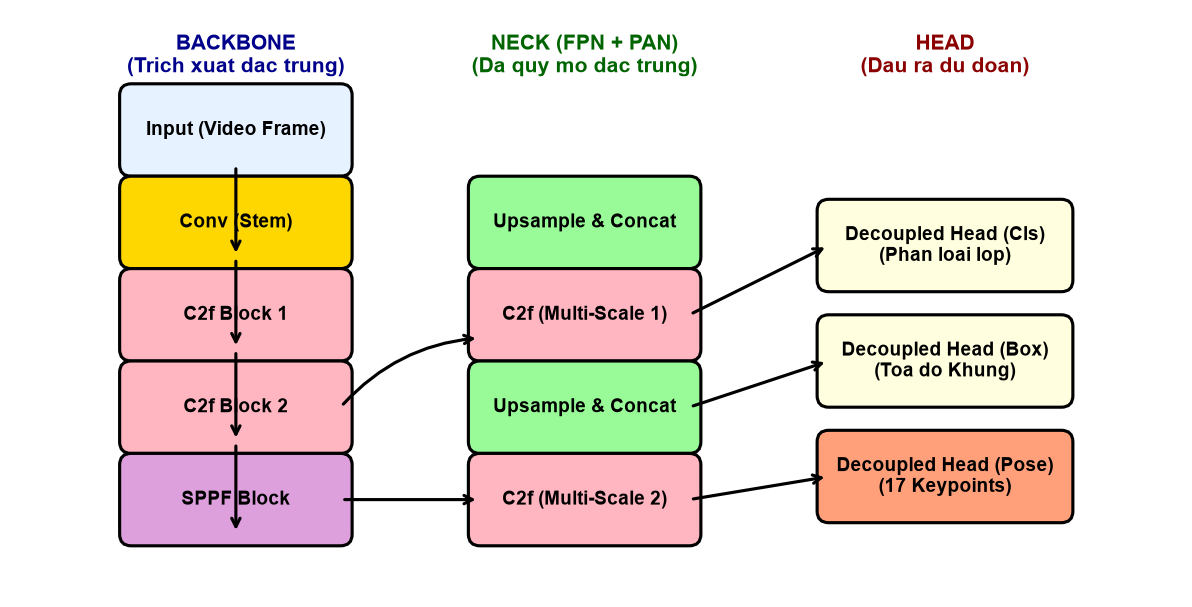
\includegraphics[width=0.95\textwidth]{Images/yolov8_architecture.png}
    \caption[Kiến trúc mạng nơ-ron tích chập YOLOv8]{\bfseries\fontsize{12pt}{0pt}\selectfont Kiến trúc mạng nơ-ron tích chập YOLOv8}
    \label{fig:yolov8_architecture}
\end{figure}

\begin{itemize}
    \item \textbf{Backbone (Mạng xương sống)}: Sử dụng kiến trúc CSPDarknet53 cải tiến, trong đó khối C3 (CSPLayer với 3 tích chập) ở các phiên bản trước được thay thế bằng khối C2f (CSPLayer với 2 tích chập nhanh). Khối C2f kết hợp các luồng đặc trưng cấp cao và cấp thấp, giúp tăng cường khả năng học biểu diễn đặc trưng đa quy mô và cải thiện dòng gradient lan truyền ngược mà không làm tăng kích thước mô hình.
    \item \textbf{Neck (Mạng cổ)}: Sử dụng cấu trúc PANet (Path Aggregation Network) kết hợp FPN (Feature Pyramid Network). Cấu trúc này giúp truyền dẫn thông tin đặc trưng ngữ cảnh từ các lớp sâu xuống các lớp nông và ngược lại. Điều này cực kỳ quan trọng đối với dữ liệu từ UAV, nơi kích thước của nạn nhân thay đổi liên tục theo độ cao bay.
    \item \textbf{Head (Đầu dự đoán)}: Điểm cải tiến cốt lõi của YOLOv8 là việc chuyển dịch từ kiến trúc dựa trên Anchor (Anchor-based) sang kiến trúc không dựa trên Anchor (Anchor-free/Anchor-less). Nhờ việc dự đoán trực tiếp tọa độ tâm và kích thước của đối tượng, mô hình giảm thiểu số lượng hộp neo cần tính toán trước, tăng tốc độ hội tụ và giảm độ phức tạp của hàm mất mát. Hơn nữa, YOLOv8 sử dụng cơ chế Decoupled Head, tách biệt nhánh dự đoán lớp (Classification) và dự đoán tọa độ (Regression), giúp nâng cao hiệu năng huấn luyện.
\end{itemize}

\subsubsection{Quy trình thu thập và tiền xử lý dữ liệu qua nền tảng Roboflow}

Nhằm đảm bảo tính hội tụ và độ chính xác của mô hình học sâu, tập dữ liệu huấn luyện cần được quản lý theo quy trình chuẩn hóa. Việc khai thác dữ liệu từ hệ sinh thái thị giác máy tính Roboflow Universe được triển khai qua các bước tiêu chuẩn như sau:

\begin{figure}[H]
    \centering
    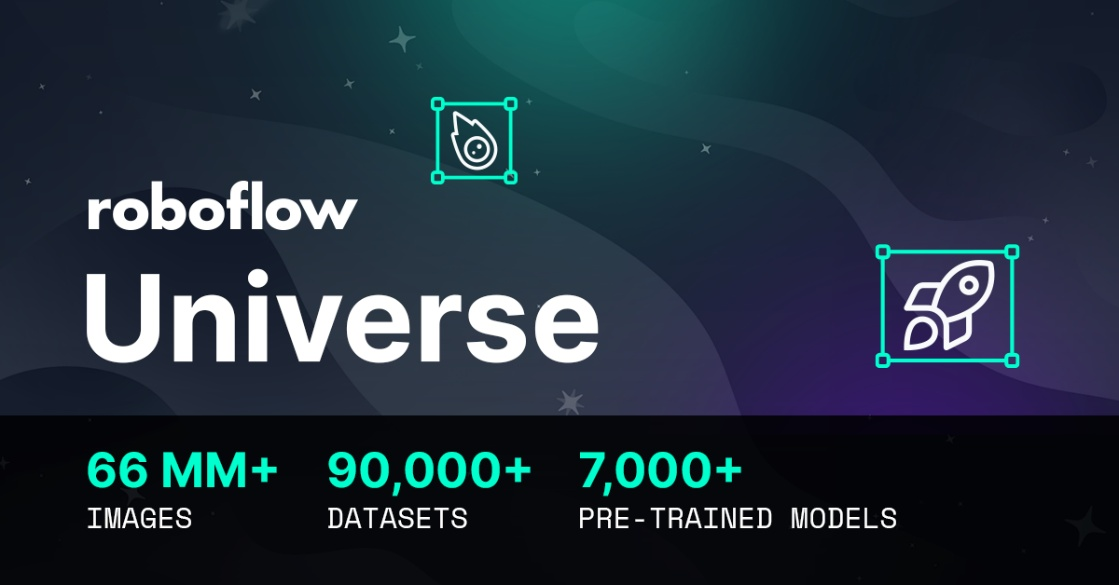
\includegraphics[width=0.85\textwidth]{Images/yolo_ai/roboflow_process.jpg}
    \caption[Quy trình tiền xử lý và tăng cường dữ liệu trên Roboflow]{\bfseries\fontsize{12pt}{0pt}\selectfont Quy trình tiền xử lý và tăng cường dữ liệu trên Roboflow}
    \label{fig:roboflow_process}
\end{figure}

\begin{itemize}
    \item \textbf{Thu thập dữ liệu}: Trích xuất các tập dữ liệu có độ phủ không gian lớn, đa dạng về bối cảnh, điều kiện ánh sáng và góc độ quan sát để tăng tính tổng quát hóa cho mô hình.
    \item \textbf{Tiền xử lý (Preprocessing)}: Đồng bộ hóa hình ảnh đầu vào, thực hiện điều chỉnh kích thước (resize) để tương thích với kiến trúc mạng YOLO (ví dụ: kích thước tiêu chuẩn $640 \times 640$ pixel).
    \item \textbf{Tăng cường dữ liệu (Data Augmentation)}: Áp dụng các phép biến đổi nhiễu động như xoay, lật hình ảnh, hoặc điều chỉnh độ sáng/độ tương phản. Kỹ thuật này mở rộng không gian mẫu hình học, giúp mô hình tăng cường khả năng kháng nhiễu và hạn chế hiện tượng học vẹt (overfitting).
    \item \textbf{Trích xuất và định dạng}: Kết xuất tập dữ liệu theo định dạng tương thích với framework YOLO. Bộ dữ liệu đầu ra bao gồm hình ảnh gốc, các tệp văn bản nhãn hóa tọa độ hộp giới hạn (bounding box), cùng tệp tin cấu hình môi trường định nghĩa rõ số lượng và tên các lớp (classes).
\end{itemize}

\subsubsection{Ứng dụng mô hình chuyên biệt YOLOv8-Rescue và YOLOv8-Posture}

Nhằm tối ưu hóa hiệu quả phát hiện nạn nhân trong môi trường thực tế phức tạp (chứa nhiều chướng ngại vật như cây cối, đổ nát, nguồn sáng phức tạp), đồ án phát triển hai mô hình chuyên biệt chạy song song trên máy trạm mặt đất:

\begin{enumerate}
    \item \textbf{Mô hình phát hiện nạn nhân (YOLOv8-Rescue)}: Được huấn luyện trên bộ dữ liệu tùy chỉnh chứa các nhãn đối tượng bao gồm: \textit{Human} (người bình thường), \textit{Victim} (nạn nhân gặp nạn), \textit{Life\_buoy} (phao cứu sinh) và \textit{Boat} (thuyền cứu hộ). Mô hình tập trung vào việc xác định vị trí và bounding box của đối tượng người trong bối cảnh cứu nạn cứu hộ.
    \item \textbf{Mô hình phân loại tư thế người (YOLOv8-Posture)}: Được tinh chỉnh (fine-tuned) để phân loại nhanh tư thế của đối tượng thành các trạng thái: \textit{Standing} (đứng), \textit{Sitting} (ngồi), \textit{Lying/Fallen} (nằm/ngã), và \textit{Collapsed} (gục, nghiêng người). Việc phân loại nhanh tư thế là tiền đề quan trọng để đánh giá mức độ khẩn cấp ban đầu.
\end{enumerate}

\subsection{Cấu trúc bộ dữ liệu huấn luyện}

Hiện tại, quá trình huấn luyện đang được tiến hành trên hai mô hình nhận diện chuyên biệt, sử dụng các tập dữ liệu đã được tổng hợp, gán nhãn và phân chia một cách có hệ thống.

\subsubsection{Tập dữ liệu Phát hiện Cứu hộ (YOLOv8-Rescue)}

Tổng khối lượng dữ liệu phục vụ bài toán phân loại và phát hiện trạng thái cứu hộ là 82.623 hình ảnh. Tập dữ liệu huấn luyện bao gồm 65.515 ảnh cung cấp các đặc trưng thị giác cốt lõi để mạng nơ-ron tối ưu hóa trọng số qua các vòng lặp. Tập kiểm thử bao gồm 10.173 ảnh độc lập được tách biệt hoàn toàn khỏi quá trình cập nhật trọng số để đánh giá khách quan hiệu năng mô hình. Cấu trúc phân vùng chi tiết của tập dữ liệu cứu hộ được tổng hợp trong Bảng \ref{tab:dataset_rescue}.

\begin{table}[H]
    \centering
    \caption[Phân vùng chi tiết tập dữ liệu huấn luyện YOLOv8-Rescue]{\bfseries\fontsize{12pt}{0pt}\selectfont Phân vùng chi tiết tập dữ liệu huấn luyện YOLOv8-Rescue}
    \begin{tabularx}{\textwidth}{|l|X|c|c|c|c|}
    \hline
    \rowcolor{LightCyan}
    \textbf{Mã DS} & \textbf{Tên tập dữ liệu gốc} & \textbf{Lớp gán} & \textbf{Ảnh Train} & \textbf{Ảnh Valid} & \textbf{Tổng cộng} \\ \hline
    ds0 & Disaster Victim v1 & 1 & 295 & 85 & 380 \\ \hline
    ds1 & Drowning Detection v1 & 0, 1 & 1.477 & 241 & 1.718 \\ \hline
    ds2 & Emergency Response v1 & 0, 1 & 1.958 & 302 & 2.260 \\ \hline
    ds3 & People Detection General & 0 & 13.449 & 2.133 & 15.582 \\ \hline
    ds4 & COCO Person v1 & 0 & 4.194 & 1.049 & 5.243 \\ \hline
    ds5 & Disaster for YOLO & 0 & 471 & 10 & 481 \\ \hline
    ds6 & Drone Person Detection & 0 & 1.870 & 274 & 2.144 \\ \hline
    ds7 & General Person Dataset & 0 & 2.314 & 997 & 3.311 \\ \hline
    ds8 & VisDrone2019 v3 & 0 & 3.946 & 481 & 4.427 \\ \hline
    ds9 & Injured People Detection & 1 & 112 & 26 & 138 \\ \hline
    ds10 & Injured People v1 & 0, 1 & 384 & 37 & 421 \\ \hline
    ds11 & People Detection Thermal & 0 & 21.422 & 3.061 & 24.483 \\ \hline
    ds13 & Rescue Dataset v1 & 1 & 405 & 38 & 443 \\ \hline
    ds14 & SOS Detection v1 & 0, 1 & 246 & 30 & 276 \\ \hline
    ds15 & Drowning Dataset v2 & 0, 1 & 8.284 & 804 & 9.088 \\ \hline
    ds16 & Rubble \& Person Detection & 0, 1 & 8.804 & 802 & 9.606 \\ \hline
    ds17 & Victim Detection v1 & 1 & 2.020 & 602 & 2.622 \\ \hline
    \end{tabularx}
    \label{tab:dataset_rescue}
\end{table}

\subsubsection{Tập dữ liệu Phân loại Tư thế (YOLOv8-Posture)}

Đối với bài toán nhận diện hành vi động học, mô hình sử dụng kho dữ liệu quy mô 19.523 hình ảnh. Tập huấn luyện chứa 16.637 ảnh chịu trách nhiệm huấn luyện mạng trích xuất đặc trưng hình thái của đối tượng ở ba trạng thái cơ bản: Đứng, Ngồi và Nằm. Tập kiểm thử bao gồm 2.886 ảnh được dùng để đo lường khách quan hiệu năng và kiểm soát hiện tượng quá khớp. Chi tiết cấu trúc tập dữ liệu tư thế được tổng hợp trong Bảng \ref{tab:dataset_posture}.

\begin{table}[H]
    \centering
    \caption[Phân vùng chi tiết tập dữ liệu huấn luyện YOLOv8-Posture]{\bfseries\fontsize{12pt}{0pt}\selectfont Phân vùng chi tiết tập dữ liệu huấn luyện YOLOv8-Posture}
    \begin{tabularx}{\textwidth}{|l|X|c|c|c|c|}
    \hline
    \rowcolor{LightCyan}
    \textbf{Mã DS} & \textbf{Tên tập dữ liệu gốc} & \textbf{Lớp gán} & \textbf{Ảnh Train} & \textbf{Ảnh Valid} & \textbf{Tổng cộng} \\ \hline
    dsA & Fall Detection v1 & 0, 1, 2 & 6.852 & 569 & 7.421 \\ \hline
    dsB & Fall Detection Raw & 2 & 3.148 & 1.349 & 4.497 \\ \hline
    dsC & Fall Down Detection & 0, 1, 2 & 3.500 & 750 & 4.250 \\ \hline
    dsE & Sitting Person v2 & 1 & 536 & 115 & 651 \\ \hline
    dsF & Person Standing & 0 & 195 & 40 & 235 \\ \hline
    dsG & Standing Person & 0 & 141 & 63 & 204 \\ \hline
    dsH & Standing Dataset & 0 & 91 & 0 & 91 \\ \hline
    dsI & Sitting Dataset & 1 & 2.174 & 0 & 2.174 \\ \hline
    \end{tabularx}
    \label{tab:dataset_posture}
\end{table}

\subsection{Ước lượng tư thế người (Pose Estimation) dựa trên YOLO-Pose}

Bên cạnh việc phát hiện bounding box, việc phân tích chi tiết tư thế hình học của cơ thể người đóng vai trò sống còn trong việc nhận diện nạn nhân đang gặp nguy hiểm (ví dụ: bị thương không thể đứng dậy, ngất xỉu). Đồ án sử dụng mô hình YOLOv8-Pose để ước lượng tư thế người thời gian thực.

\subsubsection{Nguyên lý ước lượng tư thế người và trích xuất 17 keypoints}

Mô hình YOLOv8-Pose thực hiện dự đoán đồng thời vị trí bounding box và tọa độ của 17 điểm mốc (keypoints) trên cơ thể người trong cùng một lượt quét (single-shot). Cấu trúc 17 keypoints tiêu chuẩn theo bộ dữ liệu COCO bao gồm các vị trí khớp xương chính trên cơ thể người, được minh họa trong Hình \ref{fig:yolo_pose_17_keypoints}.

\begin{figure}[H]
    \centering
    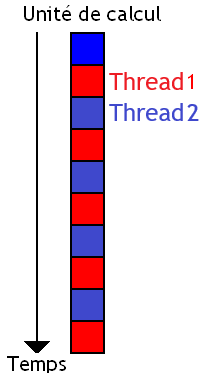
\includegraphics[width=0.55\textwidth]{Images/agent/yolo_pose_17_keypoints.png}
    \caption[Sơ đồ 17 điểm keypoints trên cơ thể người của YOLO-Pose]{\bfseries\fontsize{12pt}{0pt}\selectfont Sơ đồ 17 điểm keypoints trên cơ thể người của YOLO-Pose}
    \label{fig:yolo_pose_17_keypoints}
\end{figure}

Danh sách 17 điểm keypoints trích xuất từ mô hình bao gồm:
\begin{multicols}{2}
\begin{itemize}
    \item 0: Mũi (Nose)
    \item 1: Mắt trái (L-Eye), 2: Mắt phải (R-Eye)
    \item 3: Tai trái (L-Ear), 4: Tai phải (R-Ear)
    \item 5: Vai trái (L-Shoulder), 6: Vai phải (R-Shoulder)
    \item 7: Khuỷu tay trái (L-Elbow), 8: Khuỷu phải (R-Elbow)
    \item 9: Cổ tay trái (L-Wrist), 10: Cổ tay phải (R-Wrist)
    \item 11: Hông trái (L-Hip), 12: Hông phải (R-Hip)
    \item 13: Đầu gối trái (L-Knee), 14: Đầu gối phải (R-Knee)
    \item 15: Cổ chân trái (L-Ankle), 16: Cổ chân phải (R-Ankle)
\end{itemize}
\end{multicols}

\subsubsection{Phân tích hình học tư thế dựa trên tọa độ keypoints}

Dựa trên tọa độ pixel của 17 keypoints, thuật toán tiến hành phân tích các chỉ số hình học để tự động phát hiện trạng thái nằm/ngã (Fall/Lying detection) hoặc gục đổ (Collapsed):

\begin{itemize}
    \item \textbf{Tỷ lệ góc nghiêng thân người}: Chỉ số này được tính toán thông qua góc lệch của đường thẳng nối giữa trung điểm hai vai (trung bình cộng tọa độ vai trái và vai phải) và trung điểm hai hông (trung bình cộng tọa độ hông trái và hông phải) so với phương ngang của ảnh. Nếu góc nghiêng thân người nhỏ hơn một ngưỡng thiết lập thích hợp (cụ thể là dưới 35 độ), điều đó chứng tỏ thân người đang ở tư thế nằm ngang hoặc ngã trên mặt đất thay vì đứng thẳng (góc nghiêng thân người xấp xỉ 90 độ).
    \item \textbf{Tỷ lệ khung bao (Bounding Box Aspect Ratio)}: Định nghĩa bằng tỷ lệ giữa chiều rộng và chiều cao của hộp giới hạn bao quanh đối tượng. Đối với người đứng thẳng bình thường, chiều ngang nhỏ hơn nhiều so với chiều dọc nên tỷ lệ này thường nhỏ hơn 0.5. Khi đối tượng bị ngã hoặc nằm ra đất, chiều ngang hộp bao tăng lên rõ rệt và chiều cao giảm đi, làm tỷ lệ khung bao tăng mạnh vượt ngưỡng 1.2.
\end{itemize}

Sự kết hợp đồng thời giữa điều kiện góc nghiêng thân người nhỏ hơn 35 độ và tỷ lệ khung bao lớn hơn 1.2 cấu thành dấu hiệu hình học chắc chắn để xác định trạng thái nằm/ngã của nạn nhân với độ tin cậy cao mà không cần dựa vào các phép toán phức tạp.

\subsection{Thuật toán phân tích cử chỉ động và trạng thái nạn nhân}

Trong công tác tìm kiếm cứu hộ thực tế, nạn nhân thường cố gắng phát tín hiệu cầu cứu tới các thiết bị bay bằng cách vẫy tay. Đồng thời, những nạn nhân bị bất tỉnh sẽ nằm bất động hoàn toàn. Do đó, việc phân tích cử chỉ động theo thời gian là vô cùng cần thiết.

\subsubsection{Phát hiện cử chỉ vẫy hai tay cầu cứu (two\_hands\_waving)}

Cử chỉ vẫy hai tay cầu cứu được định nghĩa động học là sự di chuyển tuần hoàn của hai cổ tay lên phía trên đường nối hai vai theo phương dọc và có sự dao động qua lại theo phương ngang. Thuật toán lưu trữ chuỗi thời gian tọa độ của 30 khung hình gần nhất (tương đương khoảng 1.2 giây ở tốc độ xử lý 25 FPS). Quy trình phát hiện bao gồm các bước sau:

\begin{enumerate}
    \item \textbf{Chuẩn hóa tọa độ}: Để thuật toán hoạt động ổn định và độc lập với khoảng cách từ Drone đến đối tượng, tọa độ dọc của cổ tay được chuẩn hóa bằng cách lấy khoảng cách dọc từ cổ tay đến vai chia cho chiều dài thân người (khoảng cách Euclid giữa vai và hông).
    \item \textbf{Kiểm tra điều kiện biên}: Cả hai cổ tay phải nằm phía trên vai. Trong hệ tọa độ ảnh gốc (với trục dọc hướng xuống dưới), điều này tương đương với việc trị số tọa độ dọc của các cổ tay nhỏ hơn tọa độ dọc của vai tương ứng.
    \item \textbf{Phân tích tần số dao động}: Tính toán độ biến động (độ lệch chuẩn) và số lần đổi hướng chuyển động theo phương ngang của hai cổ tay trong cửa sổ thời gian. Nếu số lần đổi hướng dọc theo trục ngang vượt quá 3 lần trong cửa sổ thời gian, đồng thời biên độ dao động ngang vượt qua một ngưỡng quy định, hệ thống sẽ xác nhận có chuyển động vẫy tay.
\end{enumerate}

Nếu các điều kiện chuẩn hóa và dao động trên đồng thời được thỏa mãn trong 3 chu kỳ liên tiếp, hệ thống xác nhận nạn nhân đang thực hiện cử chỉ "Vẫy hai tay cầu cứu".

\subsubsection{Thuật toán đánh giá trạng thái bất động tĩnh (immobility)}

Đối với các nạn nhân bị chấn thương nặng hoặc bất tỉnh, trạng thái bất động tĩnh kéo dài là dấu hiệu cực kỳ nguy cấp. Thuật toán giám sát sự bất động dựa trên biến động vị trí tâm mục tiêu (Centroid) theo thời gian.

Trọng tâm mục tiêu được tính bằng trung điểm tọa độ hộp bao. Hệ thống duy trì một hàng đợi chứa các vị trí trọng tâm trong khoảng thời gian quan sát 10 giây. Độ lệch tâm tích lũy được tính bằng độ biến động (độ lệch chuẩn tổng hợp) của các tọa độ trọng tâm trong hàng đợi.

Để loại bỏ ảnh hưởng do Drone bị rung lắc hoặc di chuyển dịch chuyển camera, tọa độ trọng tâm được bù trừ dựa trên véc-tơ chuyển động nền của toàn cảnh. Véc-tơ nền này được ước lượng bằng cách tính toán dòng quang học trên các điểm đặc trưng tĩnh của mặt đất. Nếu sau khoảng thời gian quan sát, độ lệch tâm sau khi bù trừ nhỏ hơn một ngưỡng động rất nhỏ (được điều chỉnh tự động theo độ cao bay của Drone), đồng thời mô hình phân loại tư thế xác nhận đối tượng đang ở tư thế nằm, hệ thống sẽ kích hoạt trạng thái "Bất động tĩnh khẩn cấp".

\subsection{Cơ chế dung hợp quyết định (Decision Fusion) đa mô hình}

Việc chỉ sử dụng đơn lẻ một mô hình học sâu rất dễ dẫn đến hiện tượng báo động giả (false alarm). Ví dụ, một người đang nằm ngủ bình thường trên bãi cỏ hoặc một hình nhân có thể bị mô hình YOLOv8-Rescue nhận diện nhầm là nạn nhân cứu hộ. Do đó, đồ án đề xuất cơ chế dung hợp quyết định đa nguồn ở mức suy luận (inference level). Sơ đồ luồng dung hợp được thể hiện trong Hình \ref{fig:decision_fusion_flow}.

\begin{figure}[H]
    \centering
    
\includegraphics[width=0.85\textwidth]{Images/anh_cho.png}
    \caption[Sơ đồ kiến trúc dung hợp quyết định đa luồng phân tích nạn nhân]{\bfseries\fontsize{12pt}{0pt}\selectfont Sơ đồ kiến trúc dung hợp quyết định đa luồng phân tích nạn nhân}
    \label{fig:decision_fusion_flow}
\end{figure}

\subsubsection{Thuật toán dung hợp tích lũy bằng chứng xác suất nạn nhân}

Hệ thống kết hợp ba nguồn thông tin độc lập thông qua mô hình trung bình trọng số: độ tin cậy phát hiện người ($C_{rescue}$ từ YOLOv8-Rescue), xác suất phân loại tư thế nằm ngã ($P_{lying}$ từ YOLOv8-Posture) và kết quả phân tích hình học từ YOLO-Pose ($P_{pose}$).

Xác suất nạn nhân thực sự cần cứu hộ $P(Victim)$ được tính bằng tổng có trọng số của ba thông số trên. Các hệ số trọng số được tối ưu hóa qua thực nghiệm trên tập dữ liệu thử nghiệm nhằm tối đa hóa F1-score, cụ thể được thiết lập là: trọng số của mô hình phát hiện cứu hộ chiếm 0.4, mô hình phân loại tư thế chiếm 0.3, và mô hình phân tích hình học tư thế chiếm 0.3. Tổng các hệ số trọng số này luôn bảo toàn bằng 1.0 để đảm bảo xác suất đầu ra chuẩn hóa từ 0 đến 1.

\subsubsection{Thiết lập hệ thống điểm nguy cấp Danger Score}

Để trạm mặt đất có thể tự động phân loại mức độ ưu tiên cứu hộ khi có nhiều mục tiêu xuất hiện cùng lúc trên màn hình giám sát, đồ án thiết lập hệ thống điểm nguy cấp (Danger Score - $DS$) chạy từ 0 đến 100 điểm.

Công thức tính Danger Score dựa trên xác suất xác nhận nạn nhân thực tế nhân với hệ số 50, cộng thêm điểm cộng hành vi động và điểm tích lũy theo thời gian bất động tĩnh. Điểm cộng hành vi được quy định: vẫy hai tay cầu cứu cộng 30 điểm; nằm bất động cộng 40 điểm; đứng hoặc đi lại bình thường cộng 0 điểm. Điểm tích lũy thời gian bất động tăng dần theo thời gian bất động tính bằng giây chia cho 3 và giới hạn tối đa 10 điểm.

Dựa trên trị số Danger Score thu được, hệ thống tự động phân loại cảnh báo theo các cấp độ quy tắc được định nghĩa trong Bảng \ref{tab:danger_rules}.

\begin{table}[H]
    \centering
    \caption[Bảng quy tắc phân loại trạng thái cứu hộ dựa trên Danger Score]{\bfseries\fontsize{12pt}{0pt}\selectfont Bảng quy tắc phân loại trạng thái cứu hộ dựa trên Danger Score}
    \begin{tabularx}{\textwidth}{|>{\centering\arraybackslash}m{2.2cm}|>{\centering\arraybackslash}m{2.5cm}|X|X|}
    \hline
    \rowcolor{LightCyan}
    \textbf{Ngưỡng điểm DS} & \textbf{Cấp độ cảnh báo} & \textbf{Mô tả trạng thái thực tế} & \textbf{Hành động của trạm} \\ \hline
    $DS < 40$ & Bình thường (Normal) & Đối tượng di chuyển ổn định, tư thế đứng/ngồi bình thường, không có dấu hiệu khẩn cấp. & Ghi log định kỳ, không cảnh báo. \\ \hline
    $40 \le DS < 75$ & Nghi ngờ (Suspicious) & Đối tượng nằm bất động thời gian ngắn dưới 5 giây hoặc có cử chỉ lạ chưa rõ ràng. & Đổi màu khung bao sang Vàng, tăng tần số trích xuất đặc trưng. \\ \hline
    $DS \ge 75$ & Cứu trợ khẩn cấp (Danger) & Đối tượng nằm bất động kéo dài hoặc vẫy tay cầu cứu liên tục, xác suất nạn nhân cao. & Đổi màu khung bao sang Đỏ, phát âm thanh báo động, chụp ảnh lưu trữ và xuất sự kiện. \\ \hline
    \end{tabularx}
    \label{tab:danger_rules}
\end{table}

Cơ chế này đảm bảo rằng các trường hợp nạn nhân bị bất tỉnh (đạt điểm Danger Score tối đa do cộng thêm điểm bất động kéo dài) hoặc nạn nhân đang tích cực vẫy tay cầu cứu sẽ ngay lập tức được đẩy lên mức ưu tiên cao nhất, giúp tối ưu hóa thời gian vàng trong công tác tìm kiếm cứu nạn.

\subsection{Đánh giá hiệu năng huấn luyện các mô hình YOLO}

Để minh chứng cho độ tin cậy và khả năng hội tụ của các thuật toán nhận dạng được nhúng trên trạm mặt đất, hiệu năng huấn luyện của hai mô hình YOLOv8-Posture và YOLOv8-Rescue qua 50 Epochs được theo dõi và phân tích chi tiết.

\subsubsection{Đánh giá hiệu năng mô hình phân tích tư thế (YOLOv8-Posture)}

\paragraph{Phân tích dữ liệu đầu vào (Data Distribution):}
Dựa trên thống kê từ tập dữ liệu huấn luyện cho bài toán nhận diện ba trạng thái tư thế, hệ thống ghi nhận sự phân bổ không đồng đều về mặt số lượng (Class Imbalance) giữa các lớp đối tượng, thể hiện trong Hình \ref{fig:posture_data_dist}.

\begin{figure}[H]
    \centering
    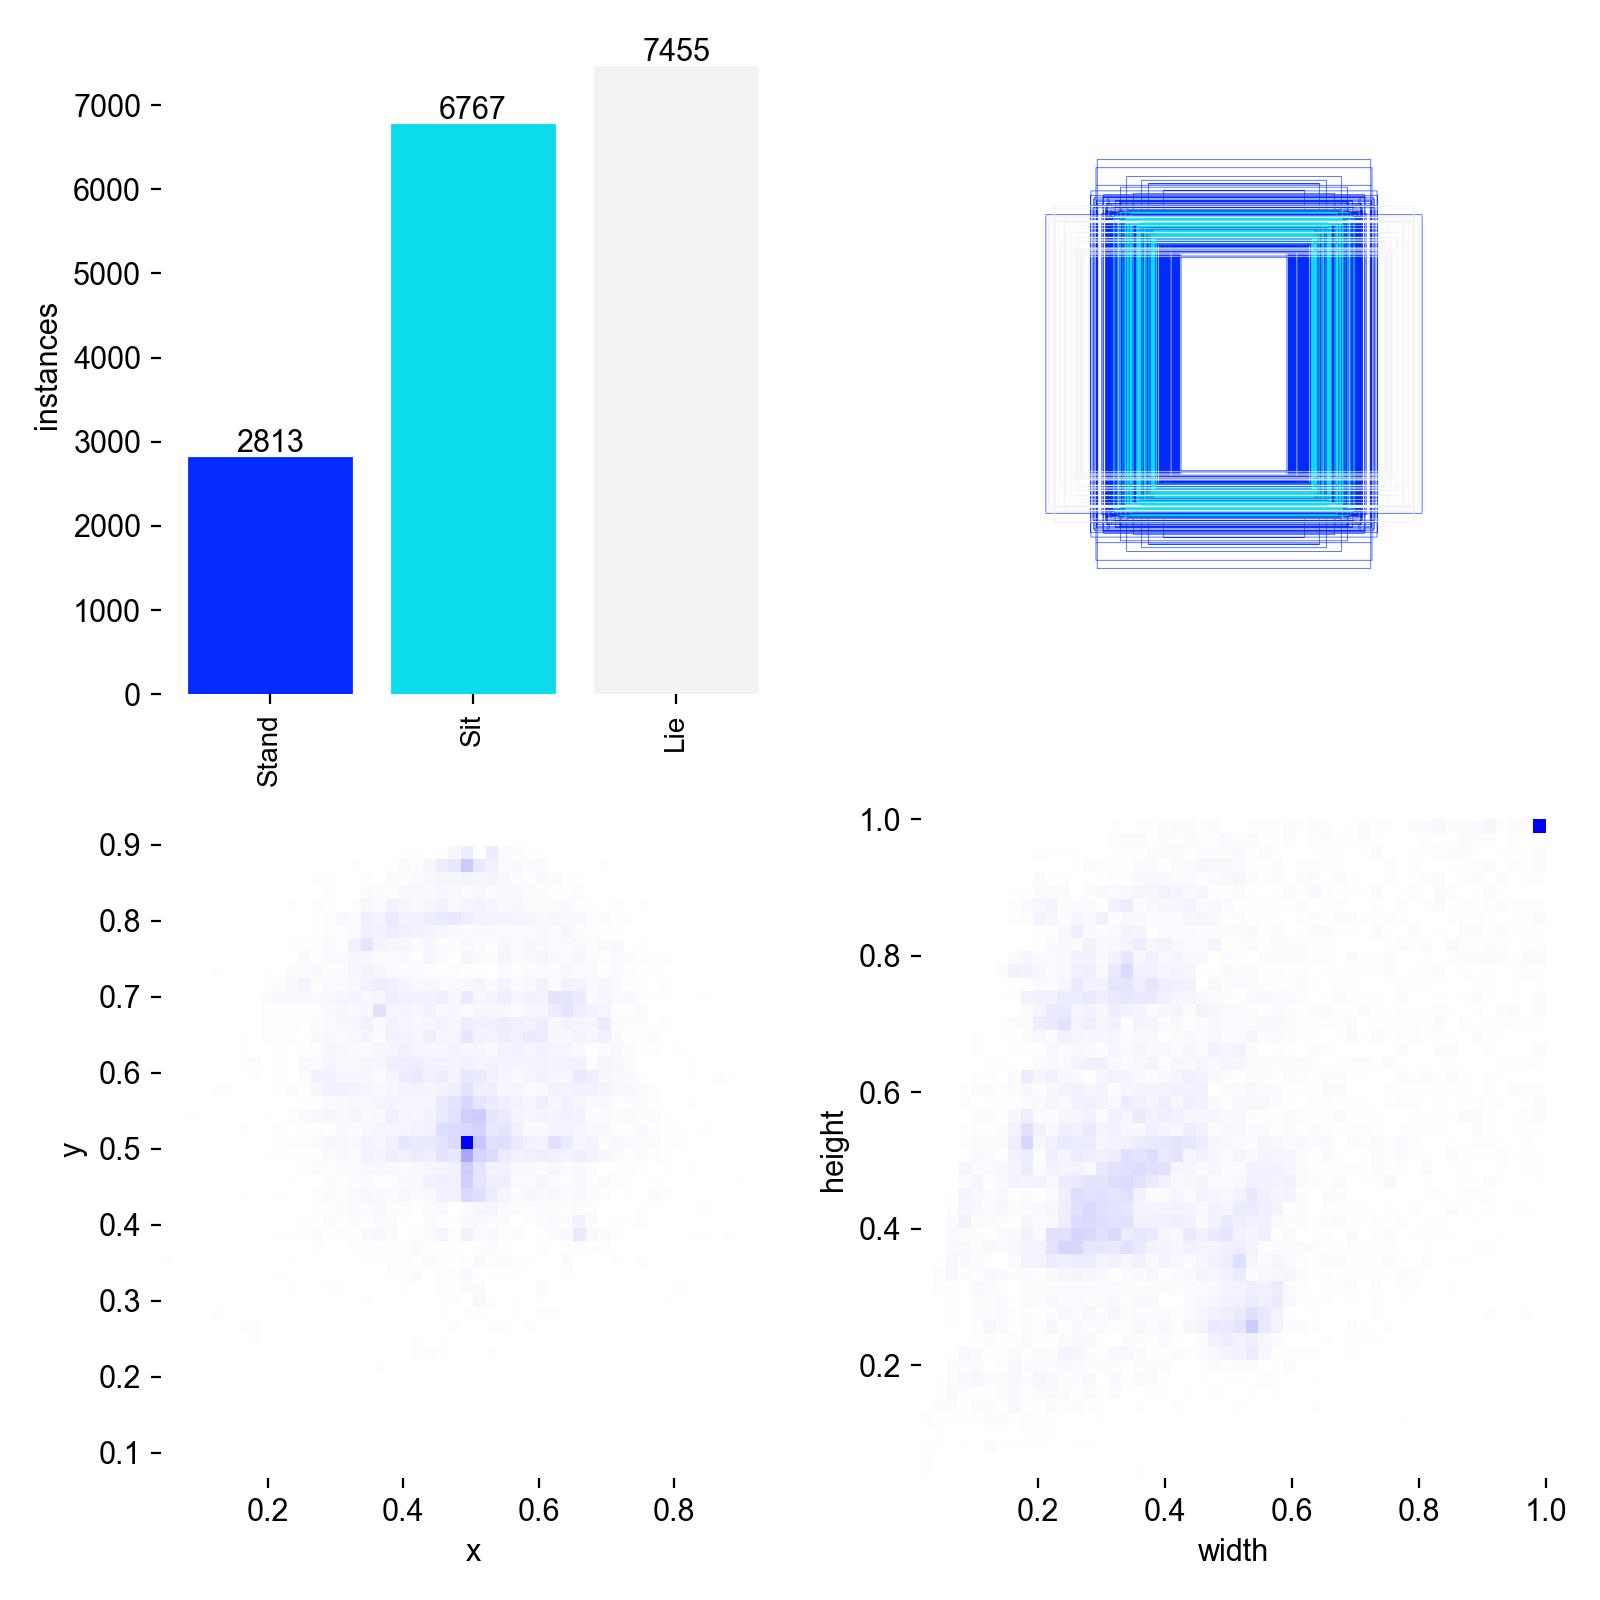
\includegraphics[width=0.65\textwidth]{Images/yolo_ai/posture_data_dist.png}
    \caption[Biểu đồ thống kê phân bổ số lượng khung giới hạn theo từng lớp tư thế]{\bfseries\fontsize{12pt}{0pt}\selectfont Biểu đồ thống kê phân bổ số lượng khung giới hạn theo từng lớp tư thế}
    \label{fig:posture_data_dist}
\end{figure}

Lớp tư thế Nằm (Lie) chiếm tỷ trọng đa số với 7.455 khung giới hạn, tiếp theo là lớp Ngồi (Sit) với 6.767 khung giới hạn, và lớp Đứng (Stand) có số lượng mẫu hạn chế nhất với 2.813 khung giới hạn. Sự chênh lệch này giải thích cho độ lệch biên trong kết quả phân loại đối với từng tư thế cụ thể của mô hình.

\paragraph{Đánh giá quá trình hội tụ (Model Convergence):}
Quá trình tối ưu hóa trọng số của mạng YOLOv8-Posture qua 50 Epochs phản ánh quỹ đạo hội tụ ổn định, thể hiện trong Hình \ref{fig:posture_loss}.

\begin{figure}[H]
    \centering
    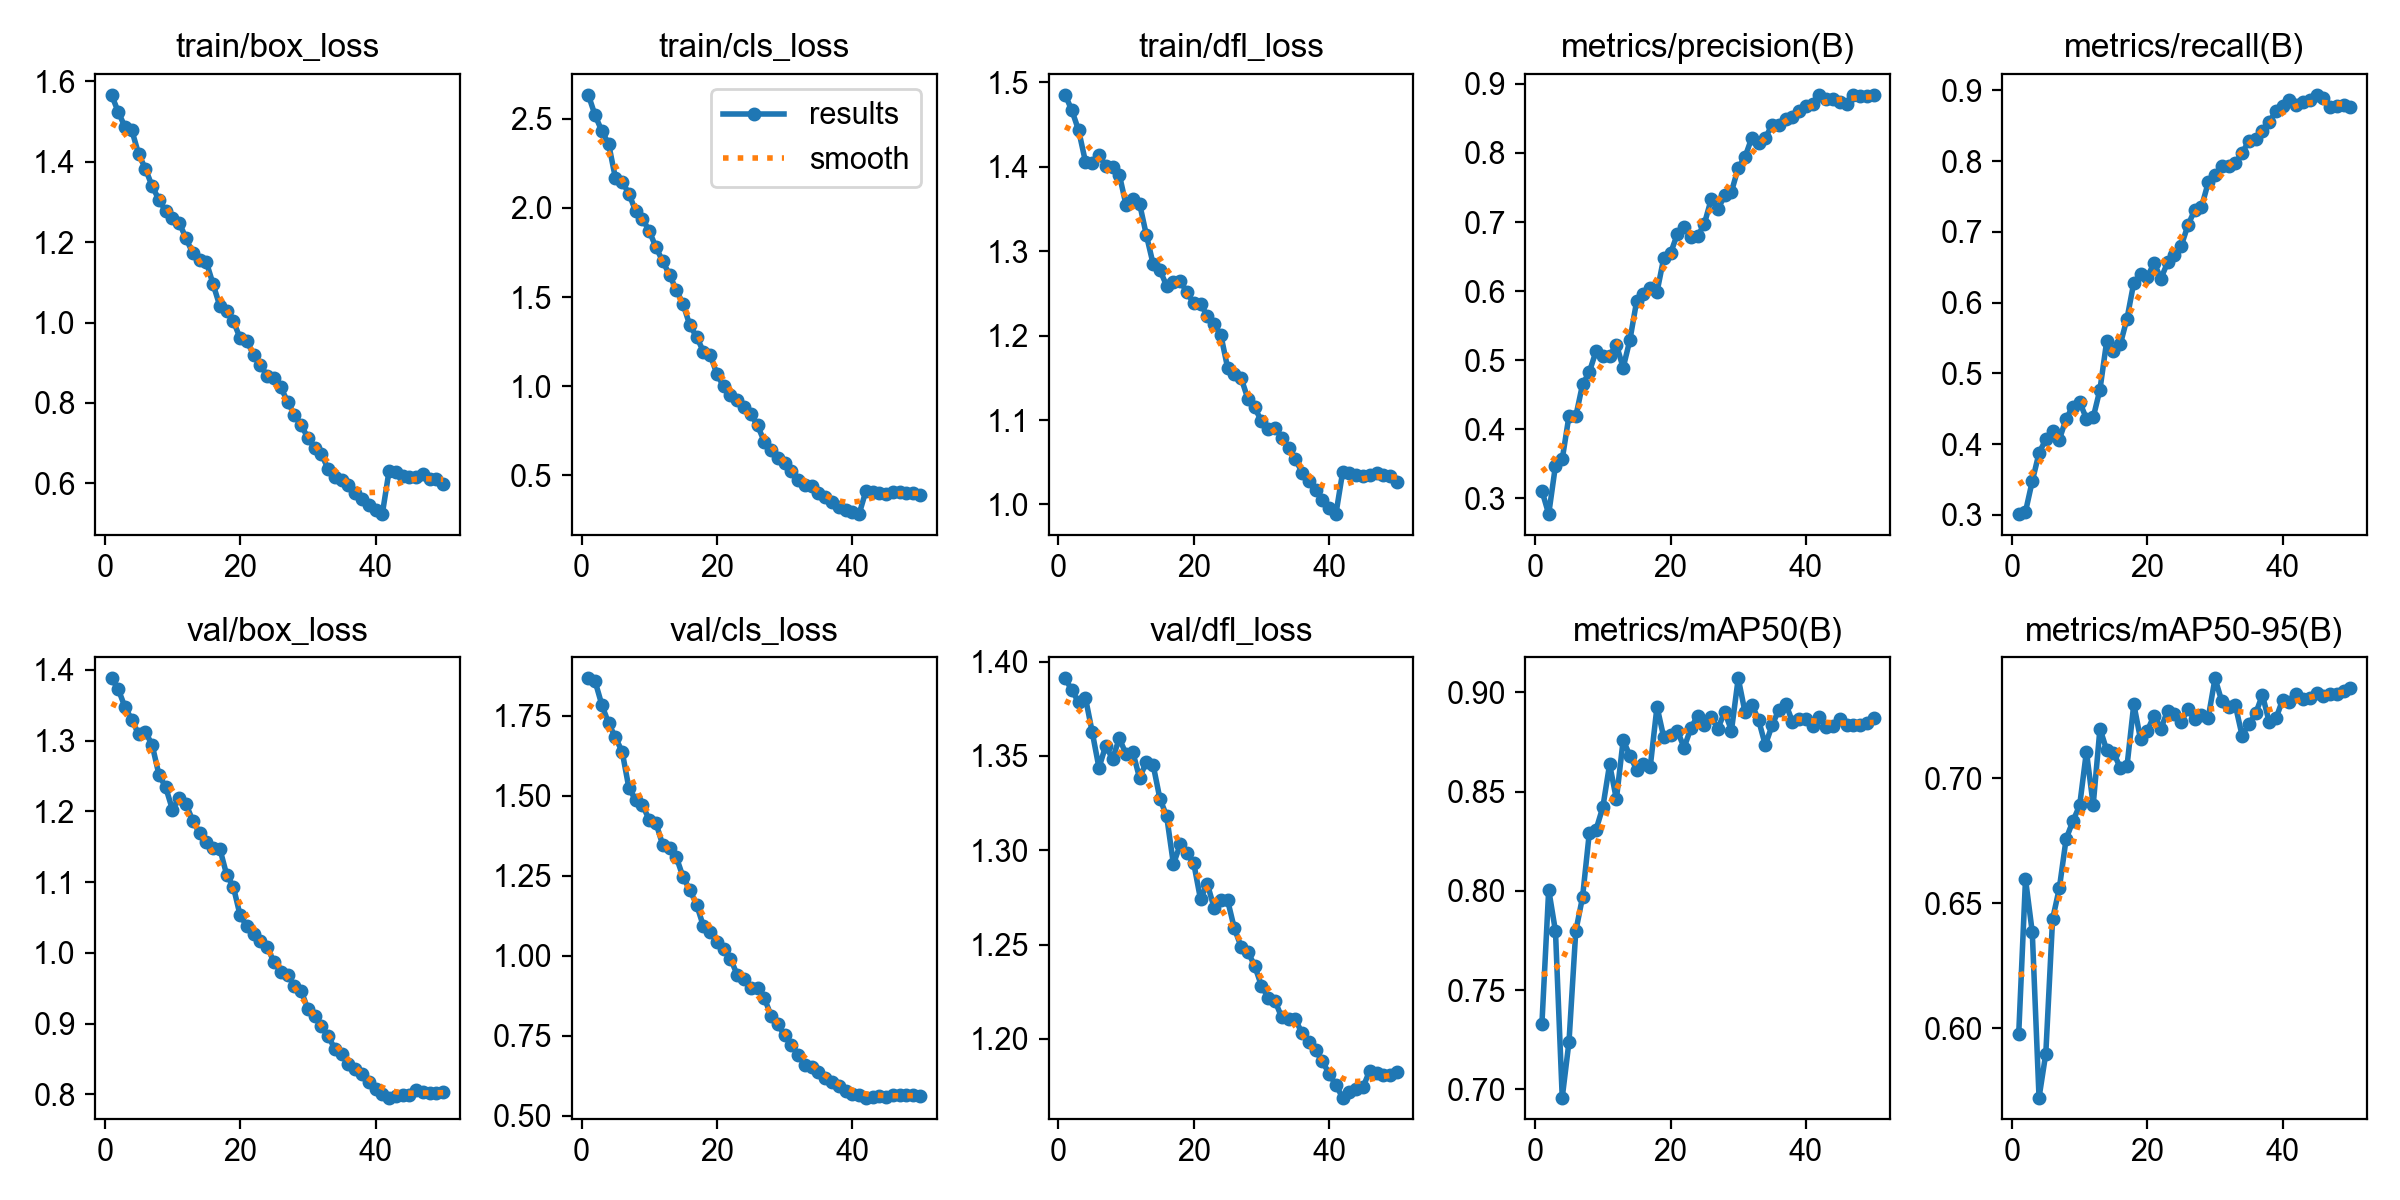
\includegraphics[width=0.75\textwidth]{Images/yolo_ai/posture_loss.png}
    \caption[Đồ thị biểu diễn hàm suy hao và chỉ số hiệu năng mô hình tư thế qua 50 Epochs]{\bfseries\fontsize{12pt}{0pt}\selectfont Đồ thị biểu diễn hàm suy hao và chỉ số hiệu năng mô hình tư thế qua 50 Epochs}
    \label{fig:posture_loss}
\end{figure}

Đường cong biểu diễn hàm suy hao trên tập huấn luyện (bao gồm box\_loss và cls\_loss) duy trì đà giảm mượt mà. Tại Epoch 50, hệ số mất mát trên tập dữ liệu kiểm thử (Validation) đạt mức tối ưu với val/box\_loss ghi nhận ở mức 0.79876 và val/cls\_loss đạt 0.56278. Sự suy giảm đồng thời giữa giá trị Train Loss và Validation Loss minh chứng năng lực tổng quát hóa tốt của mô hình, không xuất hiện trạng thái quá khớp.

\paragraph{Phân tích hiệu năng tổng thể (Overall Performance):}
Thông số kỹ thuật tại Epoch 50 chỉ ra năng lực dự báo cao của mạng nhận diện tư thế. Độ chính xác trung bình mAP@0.5 đạt mức cao 88.7\% (0.88701) và mAP@0.5:0.95 ổn định tại 73.64\% (0.73638).

\begin{figure}[H]
    \centering
    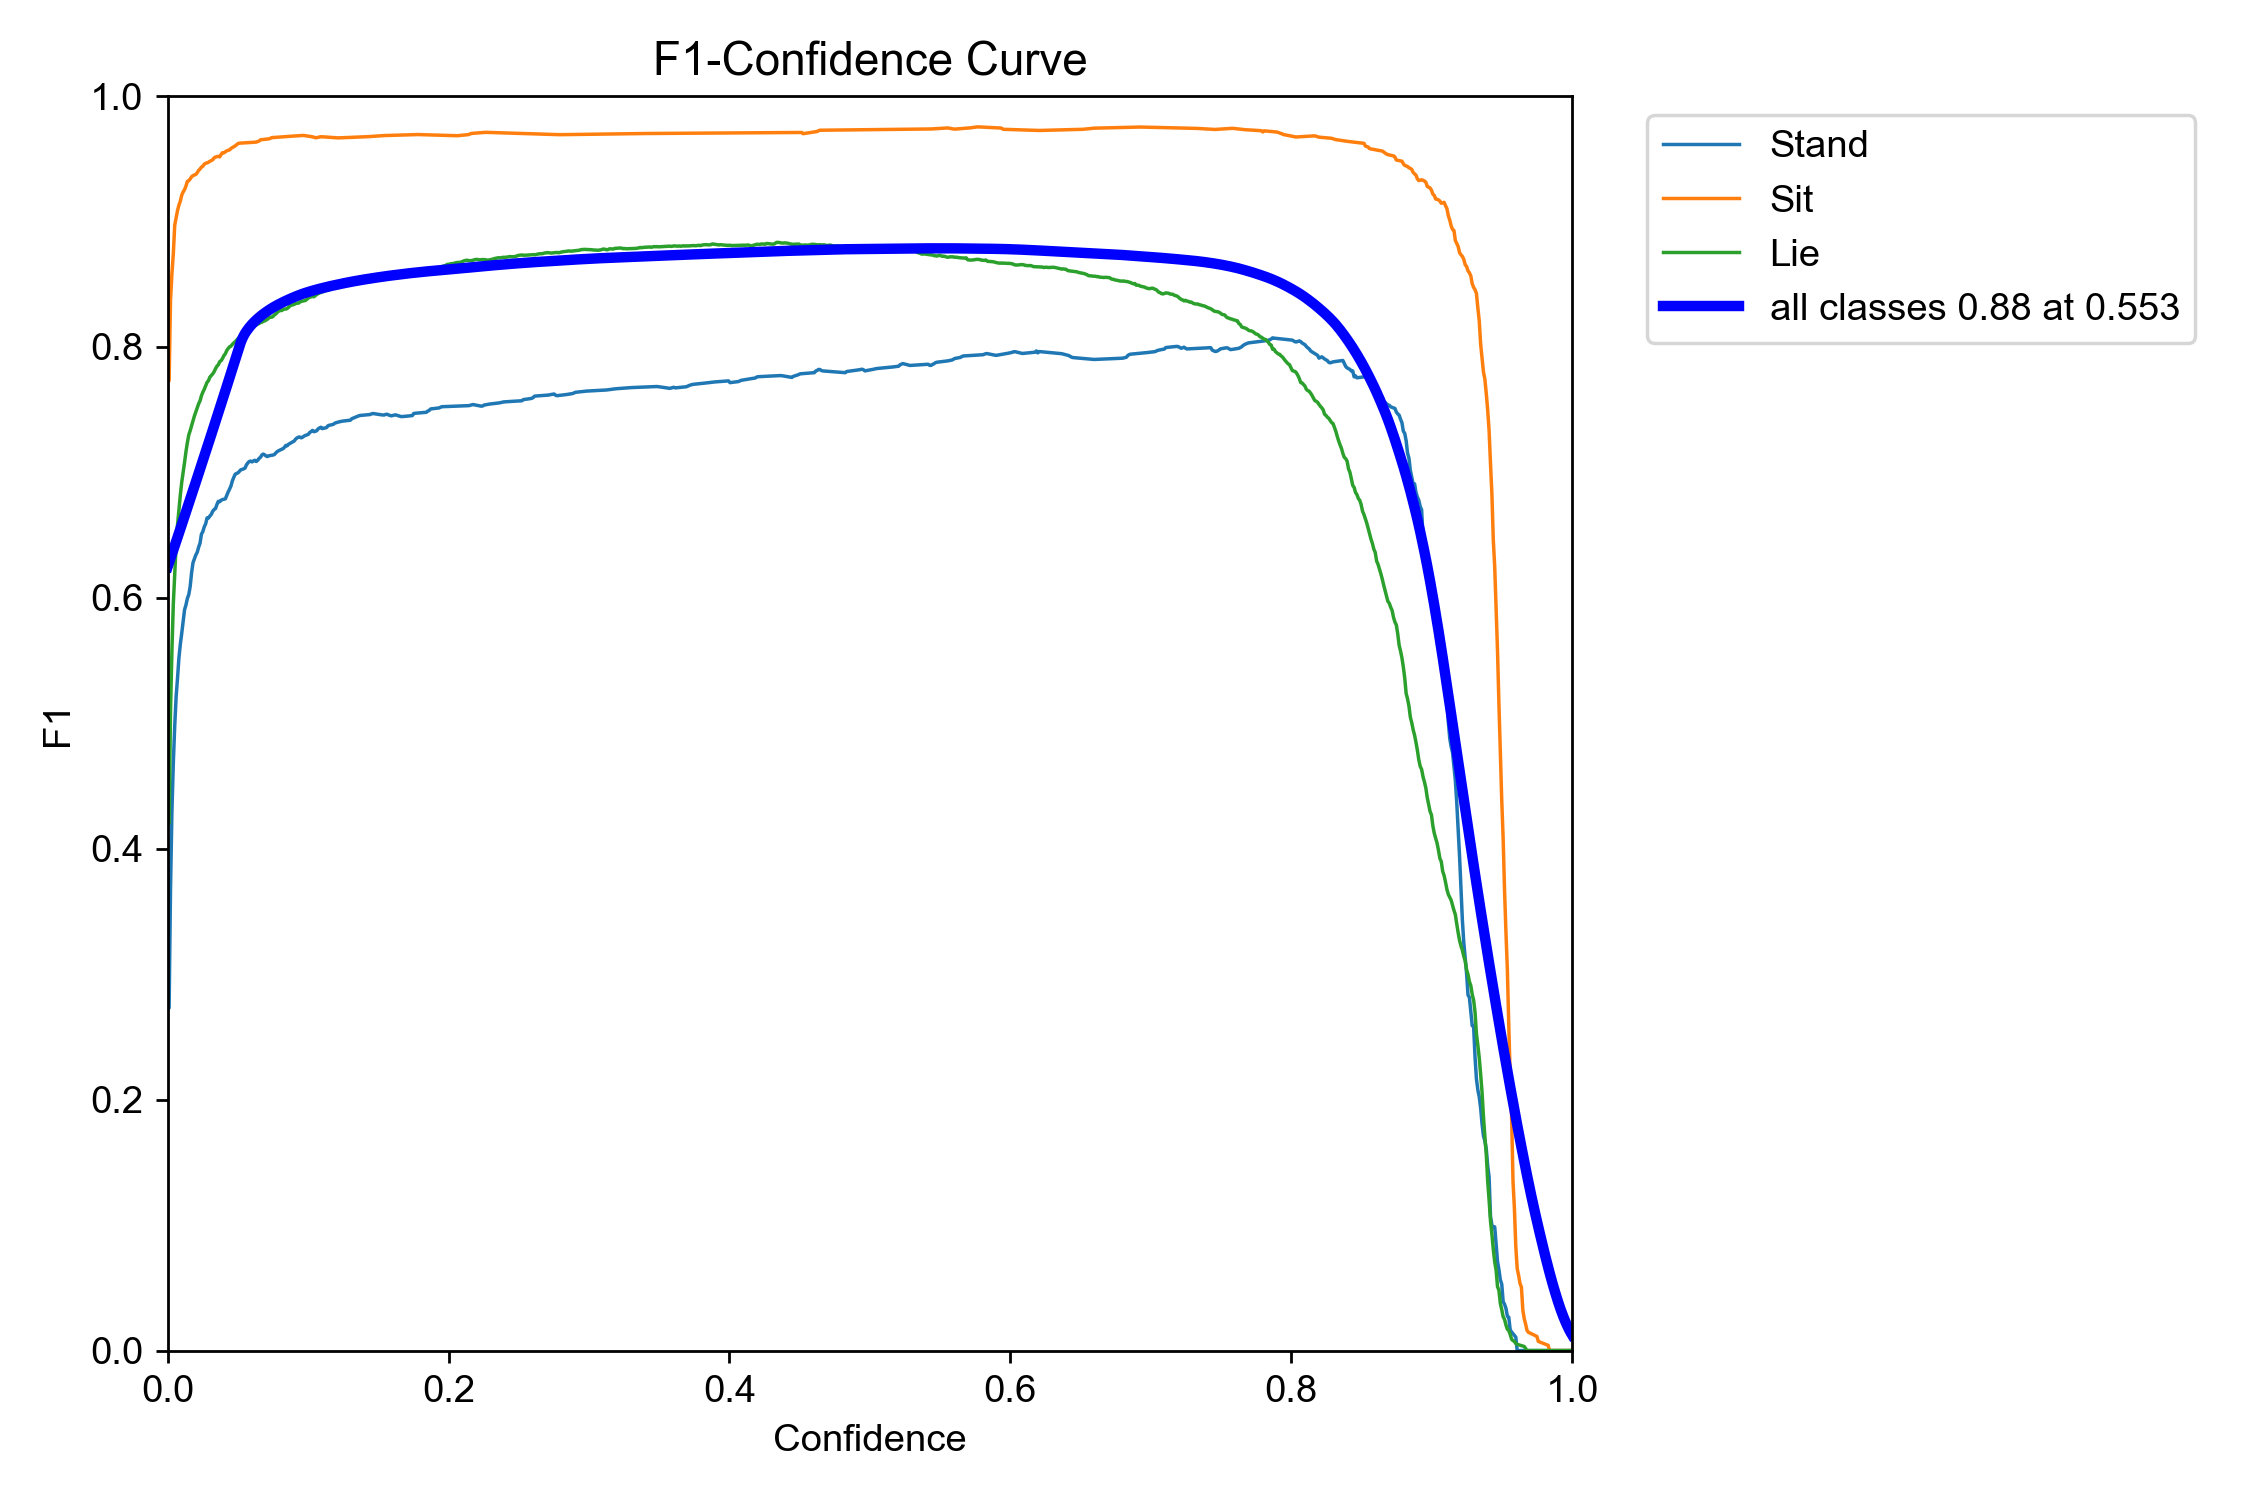
\includegraphics[width=0.65\textwidth]{Images/yolo_ai/posture_f1_curve.png}
    \caption[Đường cong F1-Confidence đánh giá sự cân bằng của mô hình tư thế]{\bfseries\fontsize{12pt}{0pt}\selectfont Đường cong F1-Confidence đánh giá sự cân bằng của mô hình tư thế}
    \label{fig:posture_f1_curve}
\end{figure}

Căn cứ trên phân tích đồ thị F1-Confidence ở Hình \ref{fig:posture_f1_curve}, chỉ số F1 tổng hợp đạt đỉnh (0.88) khi ngưỡng tin cậy (Confidence Threshold) được thiết lập tại 0.553. Đây là mức cài đặt tham chiếu khi triển khai thực tế trên máy trạm để cân bằng tối ưu giữa việc xuất hiện cảnh báo giả và việc bỏ sót mục tiêu.

\paragraph{Đánh giá độ nhạy cảm theo phân lớp (Class-Specific Performance):}
Độ nhạy cảm của thuật toán phân hóa rõ rệt đối với đặc trưng thị giác của từng lớp mục tiêu, được minh họa qua đường cong Precision-Recall ở Hình \ref{fig:posture_pr_curve} và ma trận nhầm lẫn ở Hình \ref{fig:posture_confusion_matrix}.

\begin{figure}[H]
    \centering
    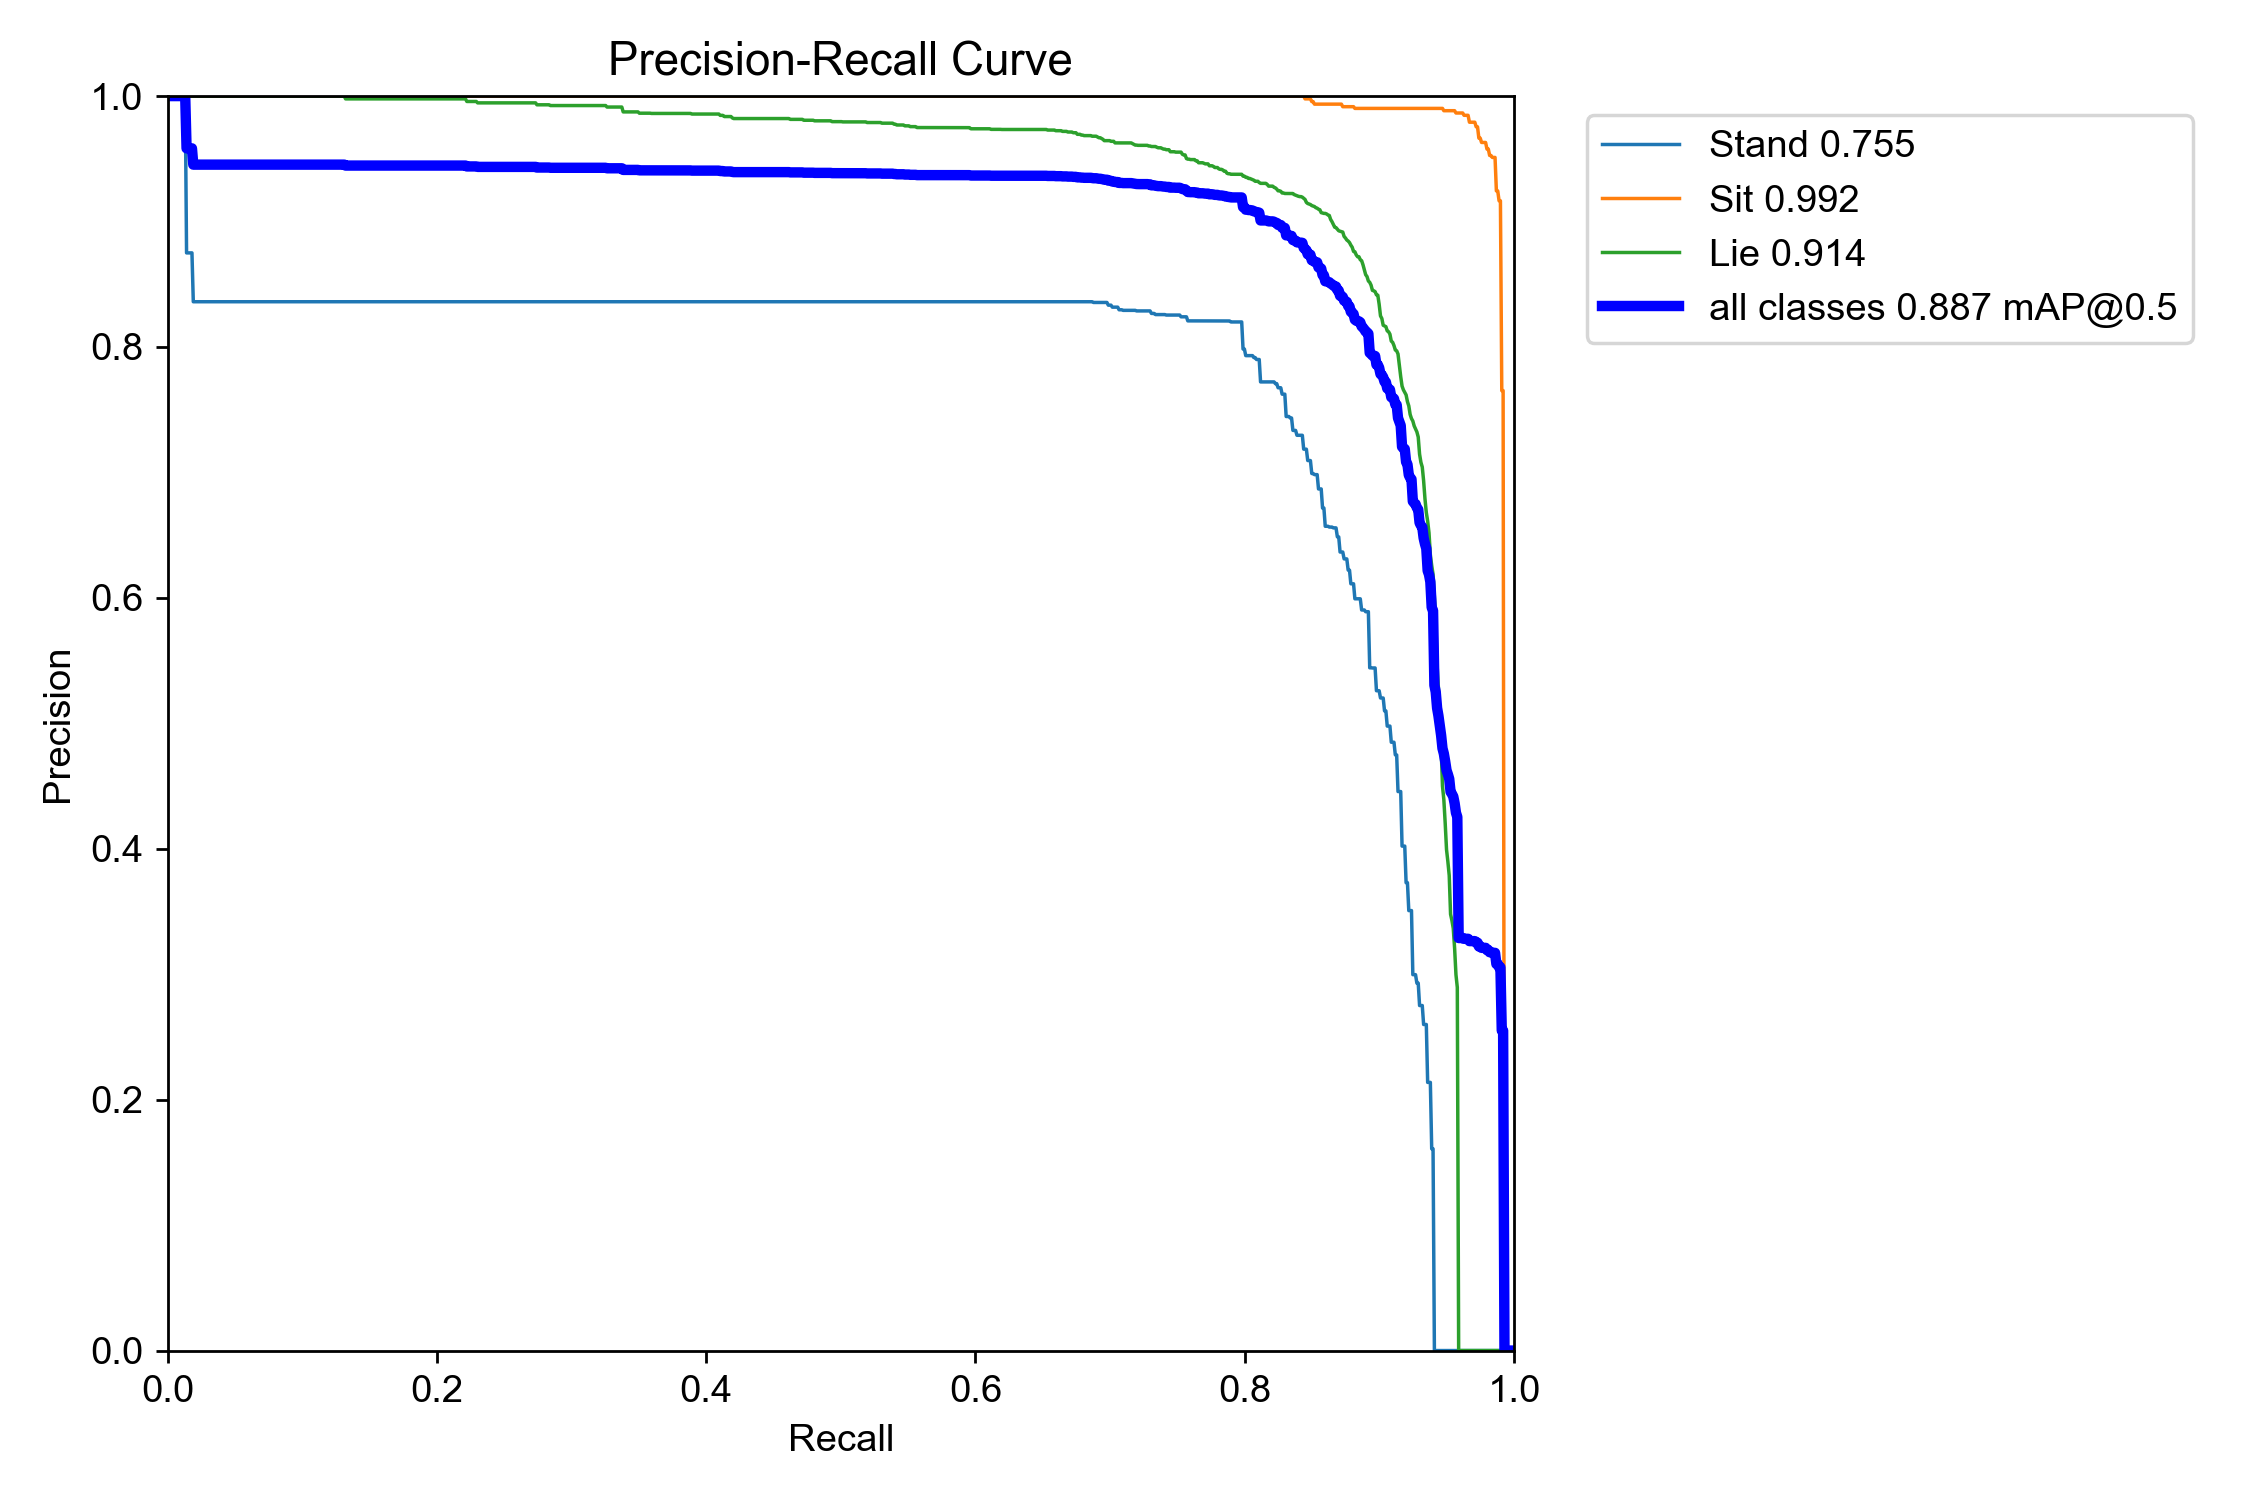
\includegraphics[width=0.65\textwidth]{Images/yolo_ai/posture_pr_curve.png}
    \caption[Đường cong Precision-Recall theo từng lớp tư thế]{\bfseries\fontsize{12pt}{0pt}\selectfont Đường cong Precision-Recall theo từng lớp tư thế}
    \label{fig:posture_pr_curve}
\end{figure}

\begin{figure}[H]
    \centering
    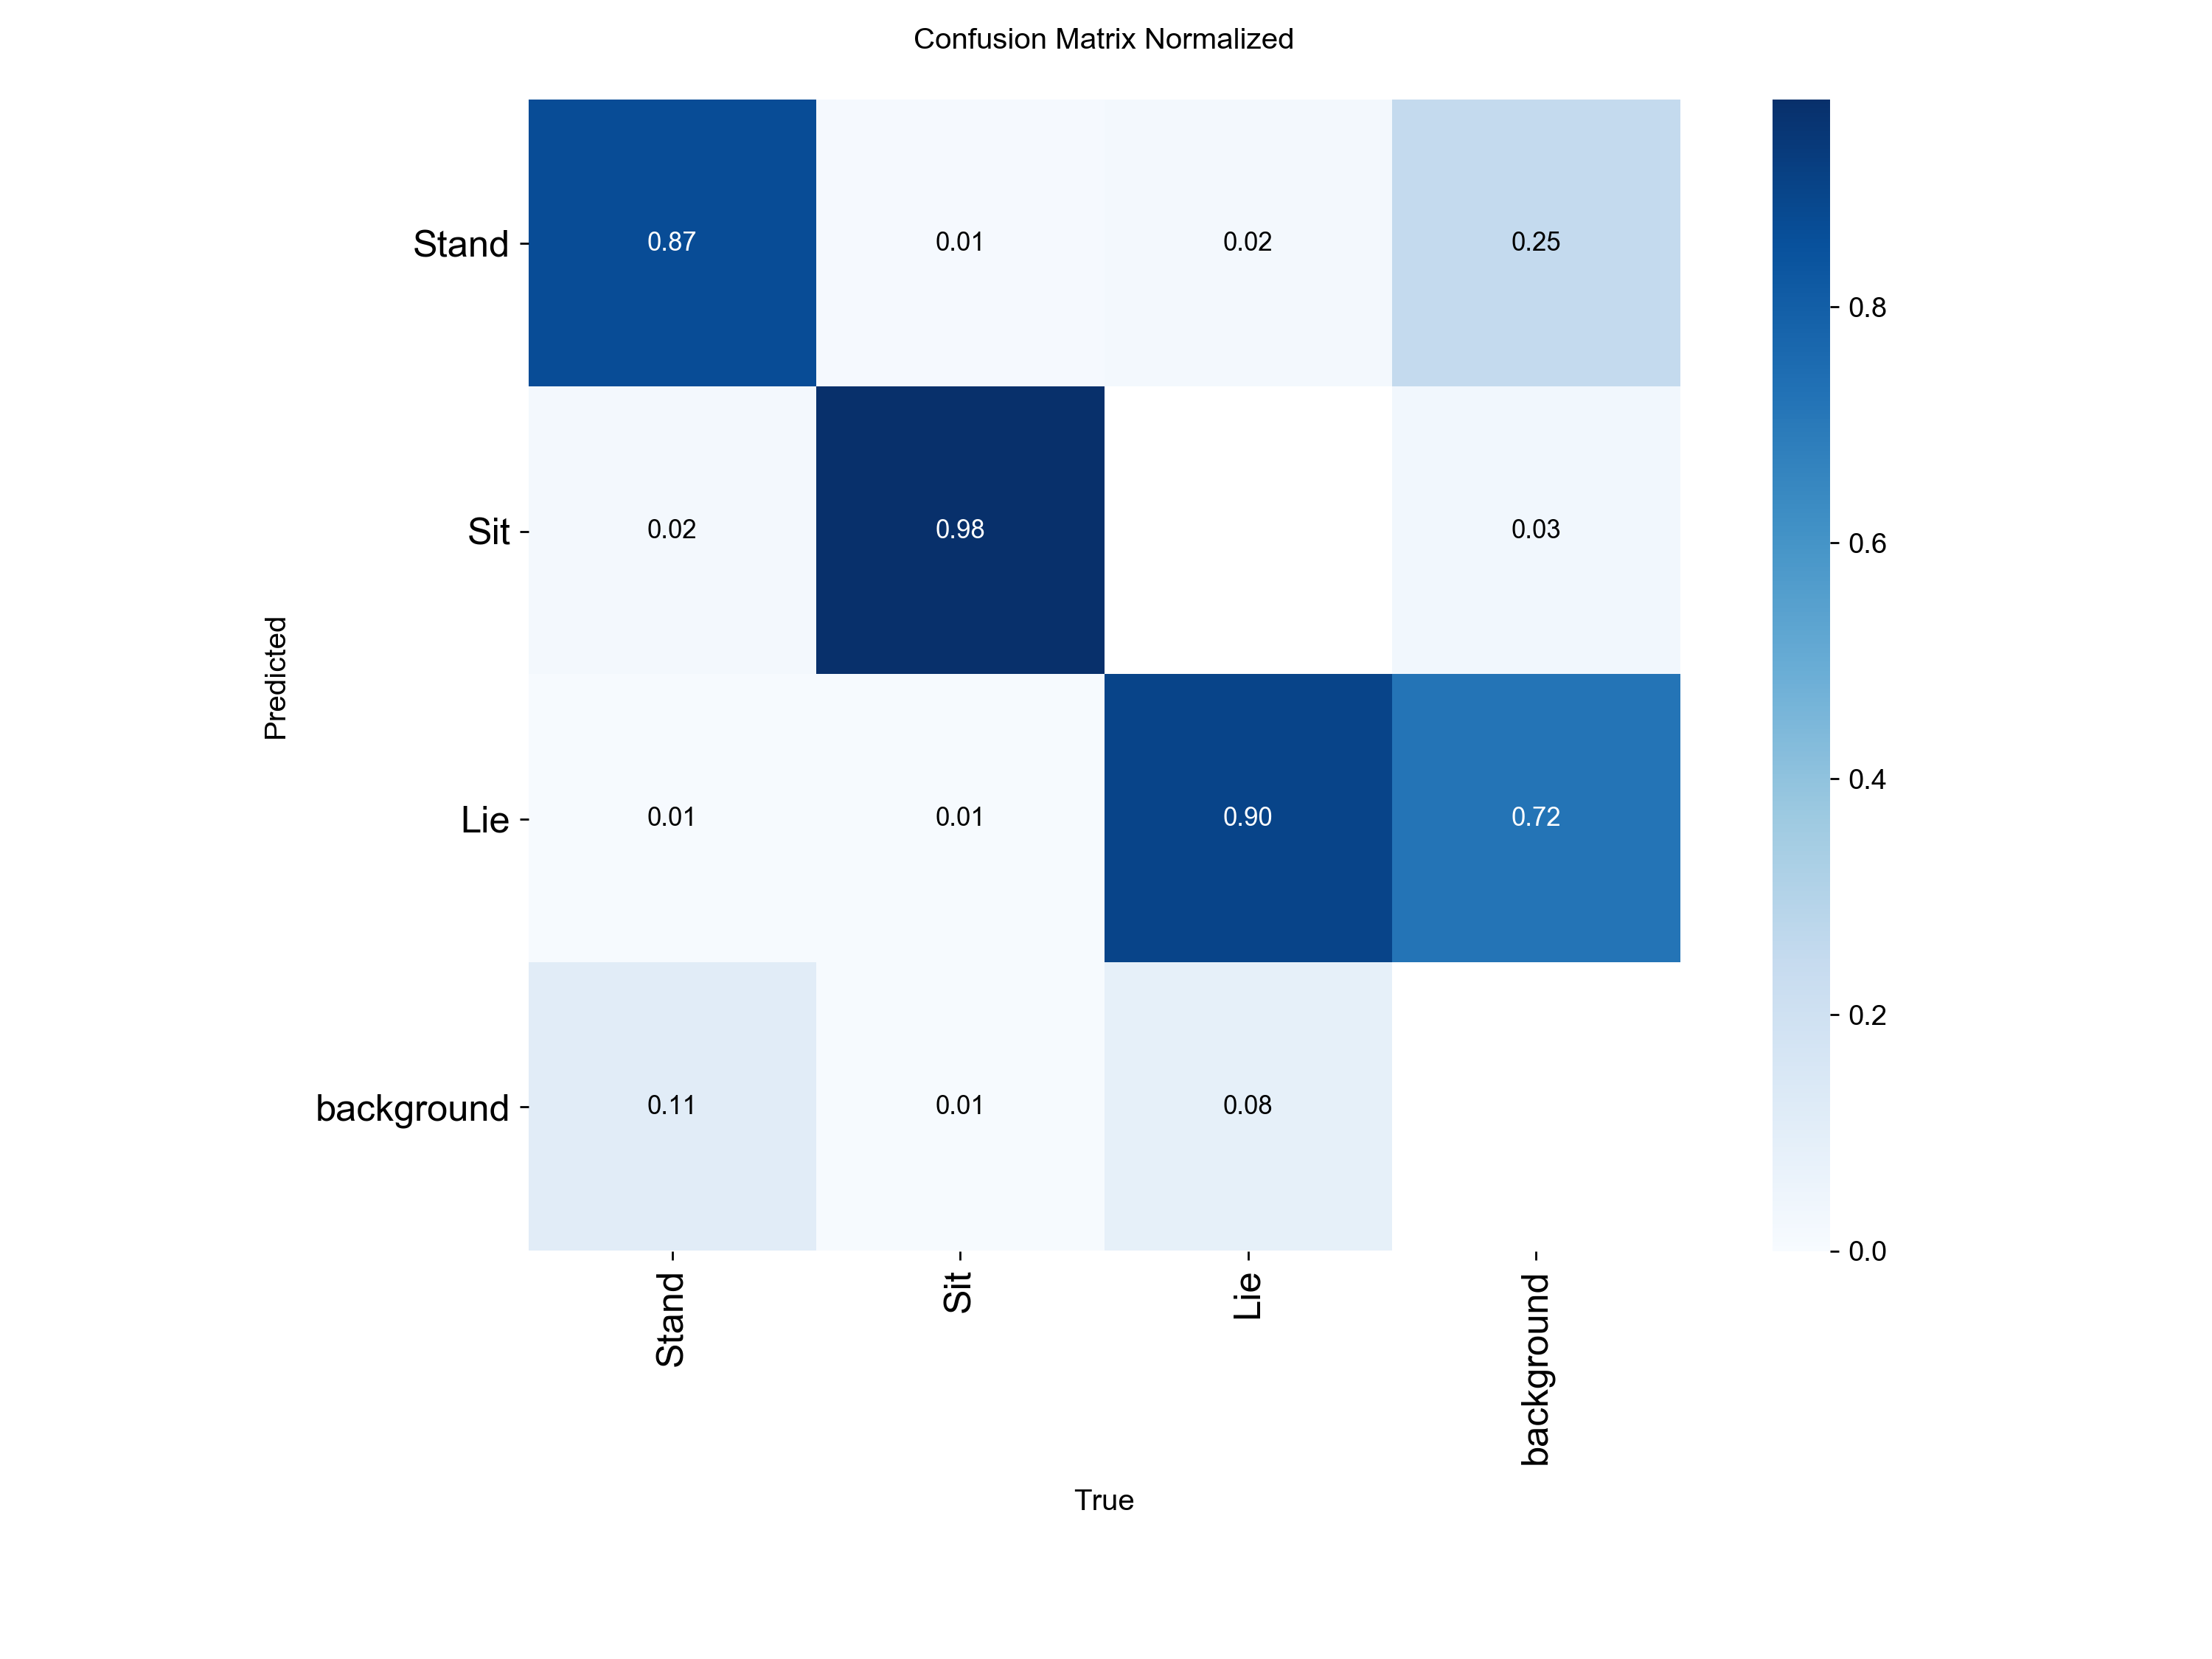
\includegraphics[width=0.6\textwidth]{Images/yolo_ai/posture_confusion_matrix.png}
    \caption[Ma trận nhầm lẫn chuẩn hóa của mô hình phân loại tư thế]{\bfseries\fontsize{12pt}{0pt}\selectfont Ma trận nhầm lẫn chuẩn hóa của mô hình phân loại tư thế}
    \label{fig:posture_confusion_matrix}
\end{figure}

Hành vi Ngồi (Sit) có khả năng nhận diện xuất sắc nhất với mAP@0.5 đạt 0.992 và tỷ lệ dự báo chính xác trong ma trận nhầm lẫn đạt 98\%. Tư thế Nằm (Lie) duy trì hiệu năng cao với chỉ số mAP@0.5 là 0.914, tỷ lệ chẩn đoán đúng đạt 90\% (khoảng 8\% bị nhầm thành nền). Tư thế Đứng (Stand) ghi nhận hiệu năng thấp nhất với mAP@0.5 ở mức 0.755 và tỷ lệ dự báo đúng đạt 87\% do số lượng mẫu huấn luyện hạn chế.

\subsubsection{Đánh giá hiệu năng mô hình phân tích cứu hộ (YOLOv8-Rescue)}

\paragraph{Phân bố dữ liệu đầu vào (Data Distribution):}
Dựa trên phân tích tập dữ liệu huấn luyện cho bài toán nhận diện trạng thái cứu hộ, hệ thống ghi nhận sự mất cân bằng dữ liệu cực kỳ lớn (Extreme Class Imbalance) giữa lớp người bình thường và nạn nhân gặp nạn, thể hiện trong Hình \ref{fig:rescue_data_dist}.

\begin{figure}[H]
    \centering
    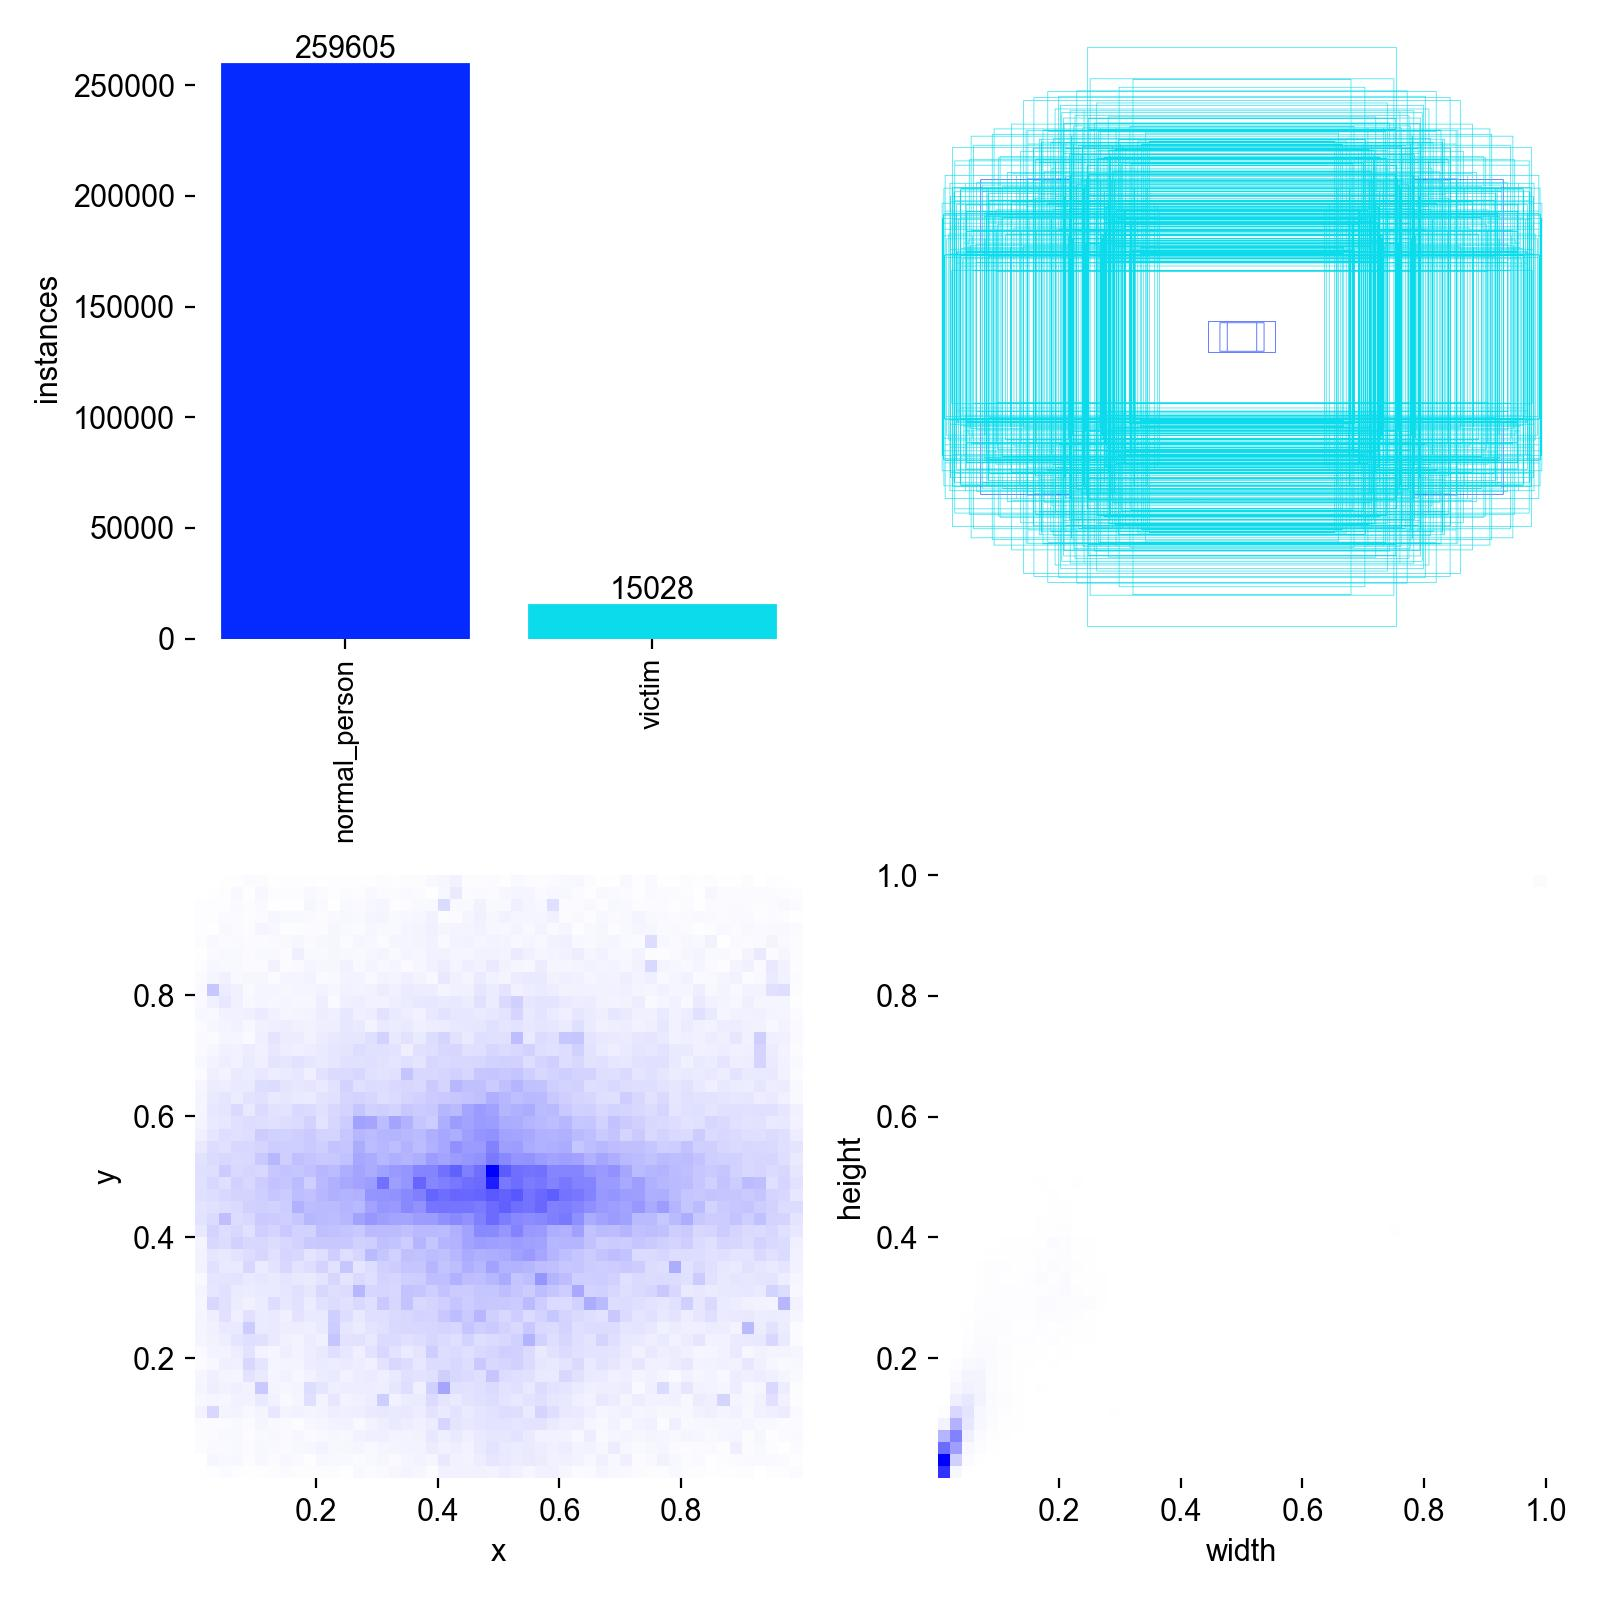
\includegraphics[width=0.65\textwidth]{Images/yolo_ai/rescue_data_dist.jpg}
    \caption[Biểu đồ thống kê phân bổ số lượng khung giới hạn theo lớp Normal và Victim]{\bfseries\fontsize{12pt}{0pt}\selectfont Biểu đồ thống kê phân bổ số lượng khung giới hạn theo lớp Normal và Victim}
    \label{fig:rescue_data_dist}
\end{figure}

Lớp người bình thường (Normal) chiếm tỷ trọng áp đảo tuyệt đối với 114.121 khung giới hạn, trong khi lớp nạn nhân (Victim) chỉ ghi nhận vỏn vẹn 5.085 khung giới hạn (tỷ lệ lệch xấp xỉ 22:1). Đây là thách thức lớn, dễ khiến mô hình học thiên lệch sang lớp đa số.

\paragraph{Đánh giá quá trình hội tụ (Model Convergence):}
Đồ thị tối ưu hóa trọng số của mạng YOLOv8-Rescue qua 50 Epochs chỉ ra mô hình đạt đến trạng thái bão hòa, thể hiện trong Hình \ref{fig:rescue_loss}.

\begin{figure}[H]
    \centering
    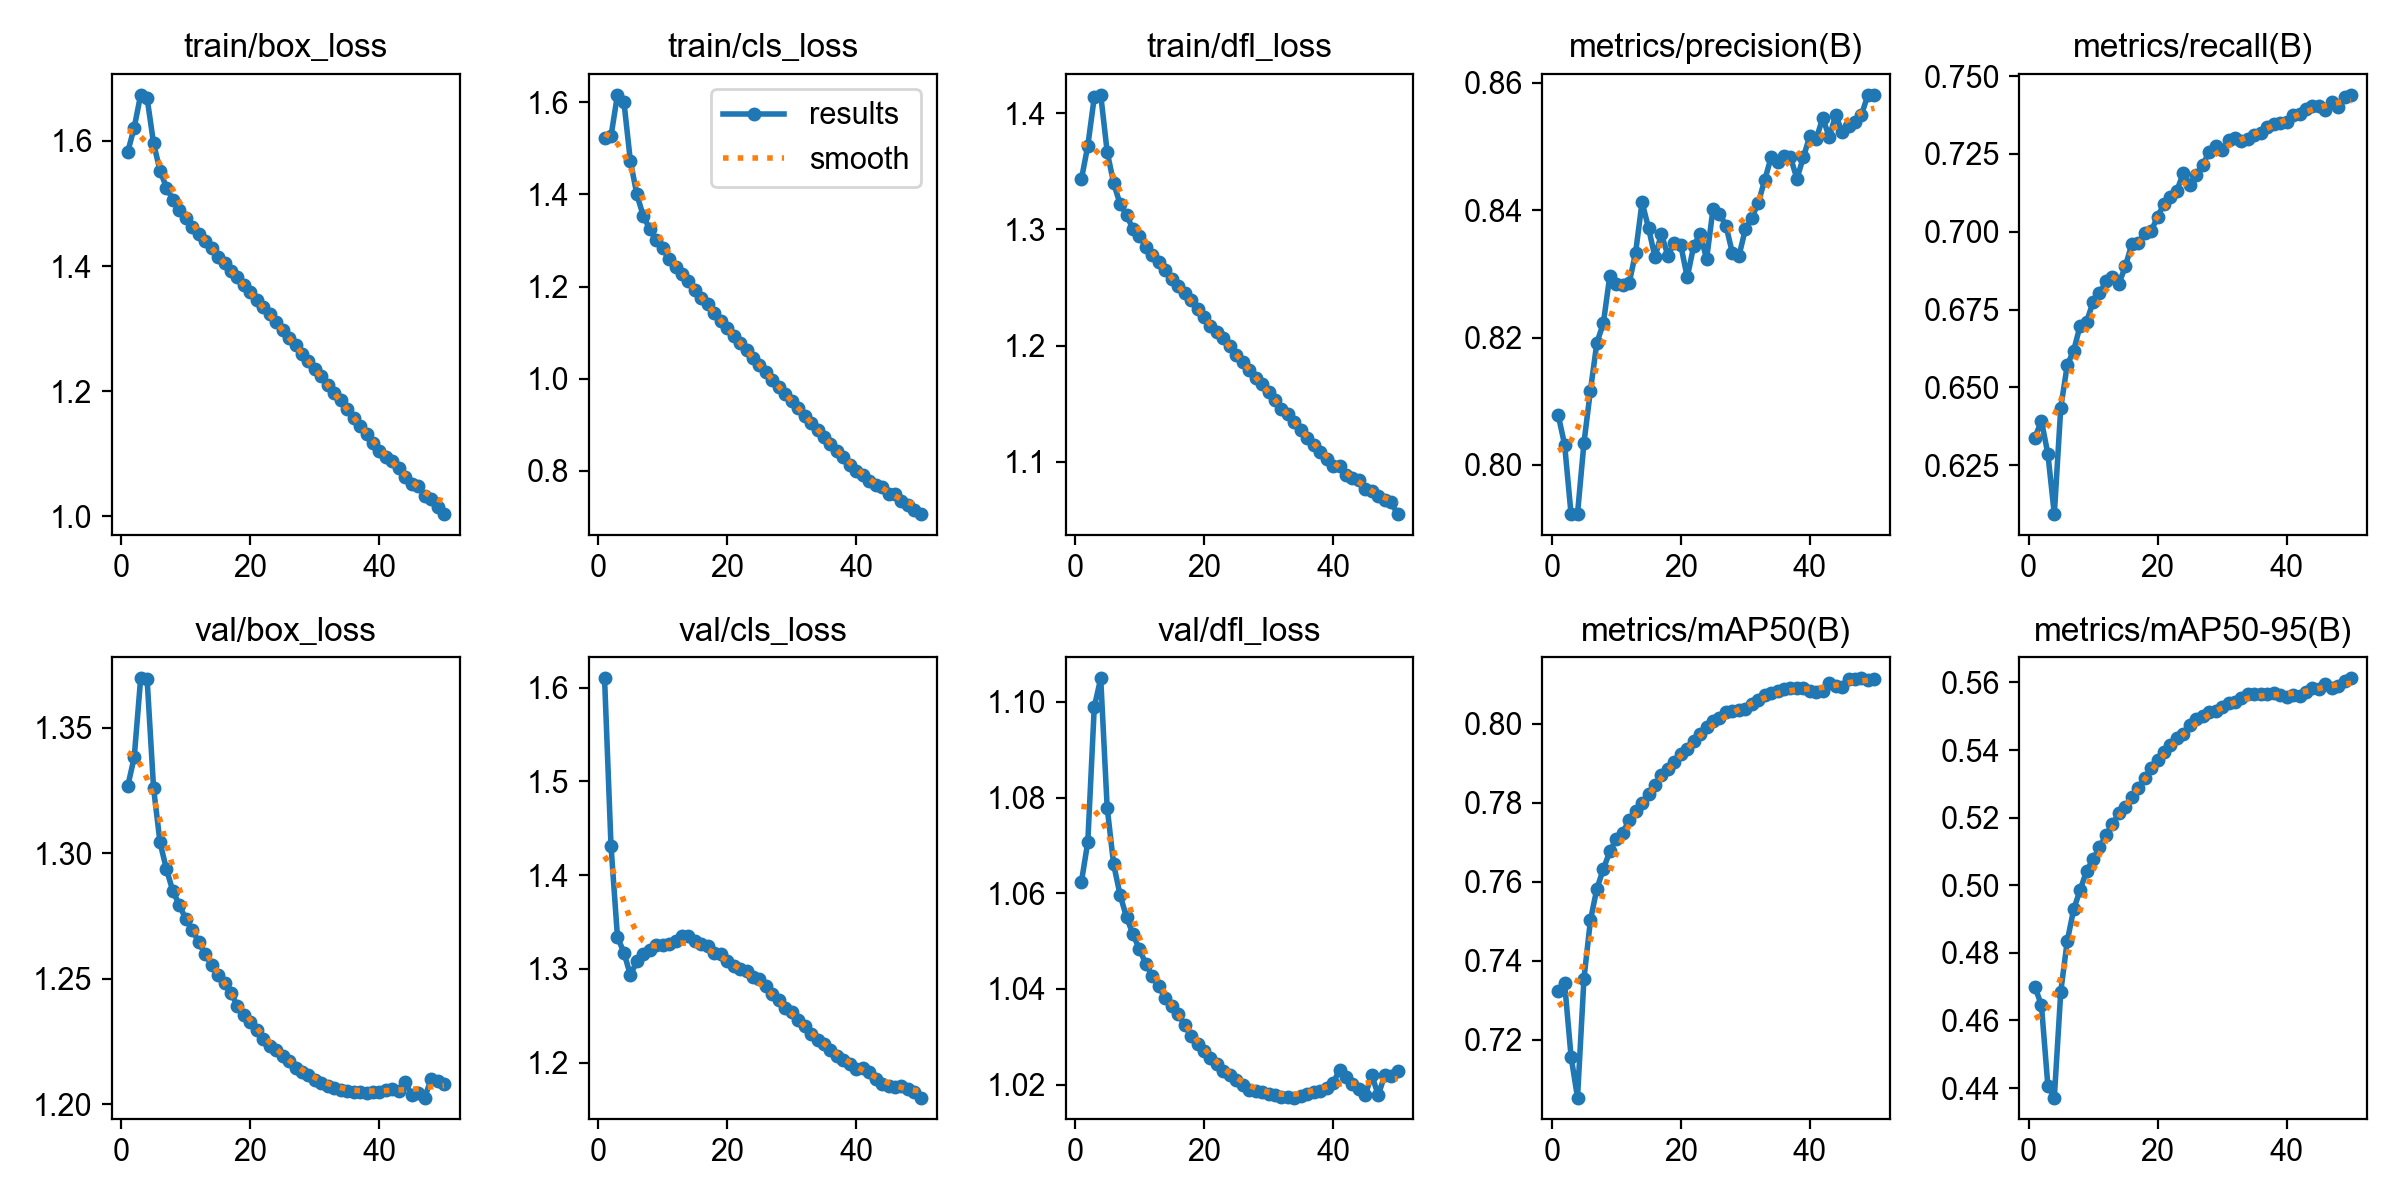
\includegraphics[width=0.75\textwidth]{Images/yolo_ai/rescue_loss.png}
    \caption[Đồ thị biểu diễn hàm suy hao và chỉ số hiệu năng mô hình cứu hộ qua 50 Epochs]{\bfseries\fontsize{12pt}{0pt}\selectfont Đồ thị biểu diễn hàm suy hao và chỉ số hiệu năng mô hình cứu hộ qua 50 Epochs}
    \label{fig:rescue_loss}
\end{figure}

Đường cong hàm suy hao trên tập huấn luyện tiếp tục giảm dần đều đến Epoch 50. Tuy nhiên, trên tập kiểm thử (Validation), đường cong suy hao val/box\_loss và val/cls\_loss bắt đầu đi ngang từ khoảng Epoch 30 đến 40 và không giảm thêm, cho thấy mô hình đã đạt ngưỡng giới hạn hội tụ tối đa với tập dữ liệu hiện hành.

\paragraph{Phân tích hiệu năng tổng thể (Overall Performance):}
Thông số kỹ thuật đánh giá tổng thể cho thấy hệ thống chịu ảnh hưởng nhất định từ sự mất cân bằng dữ liệu đầu vào, thể hiện qua đường F1-Confidence ở Hình \ref{fig:rescue_f1_curve} và Precision-Recall ở Hình \ref{fig:rescue_pr_curve}.

\begin{figure}[H]
    \centering
    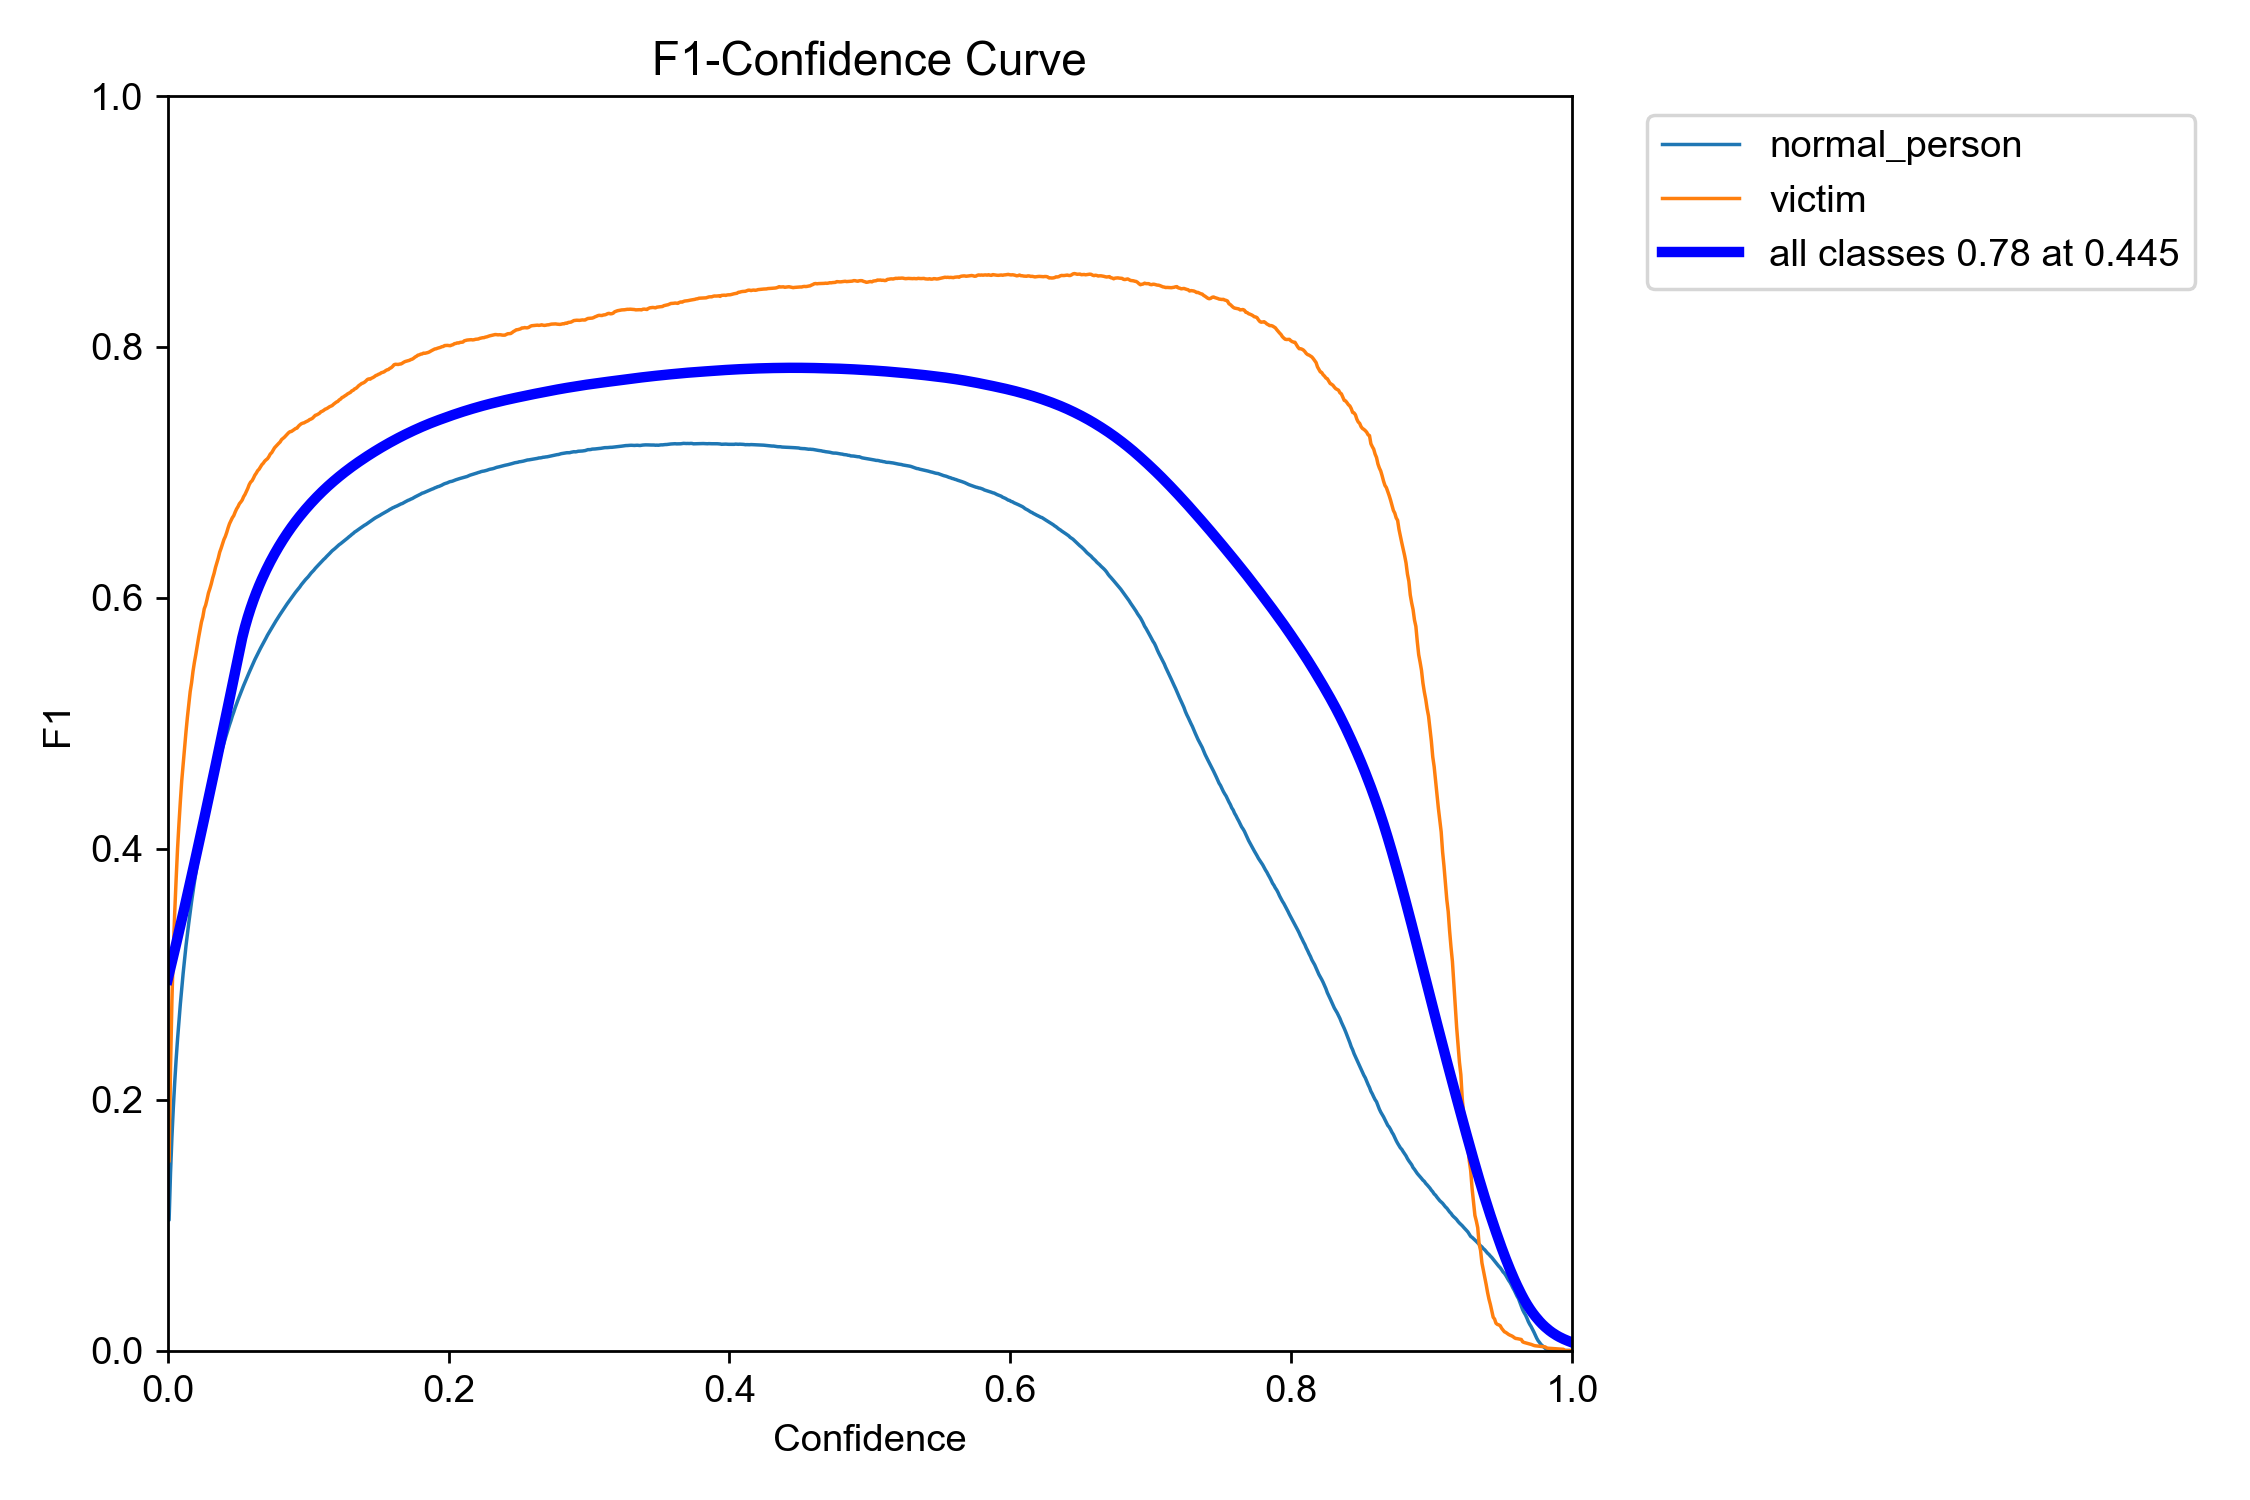
\includegraphics[width=0.65\textwidth]{Images/yolo_ai/rescue_f1_curve.png}
    \caption[Đường cong F1-Confidence đánh giá sự cân bằng của mô hình cứu hộ]{\bfseries\fontsize{12pt}{0pt}\selectfont Đường cong F1-Confidence đánh giá sự cân bằng của mô hình cứu hộ}
    \label{fig:rescue_f1_curve}
\end{figure}

\begin{figure}[H]
    \centering
    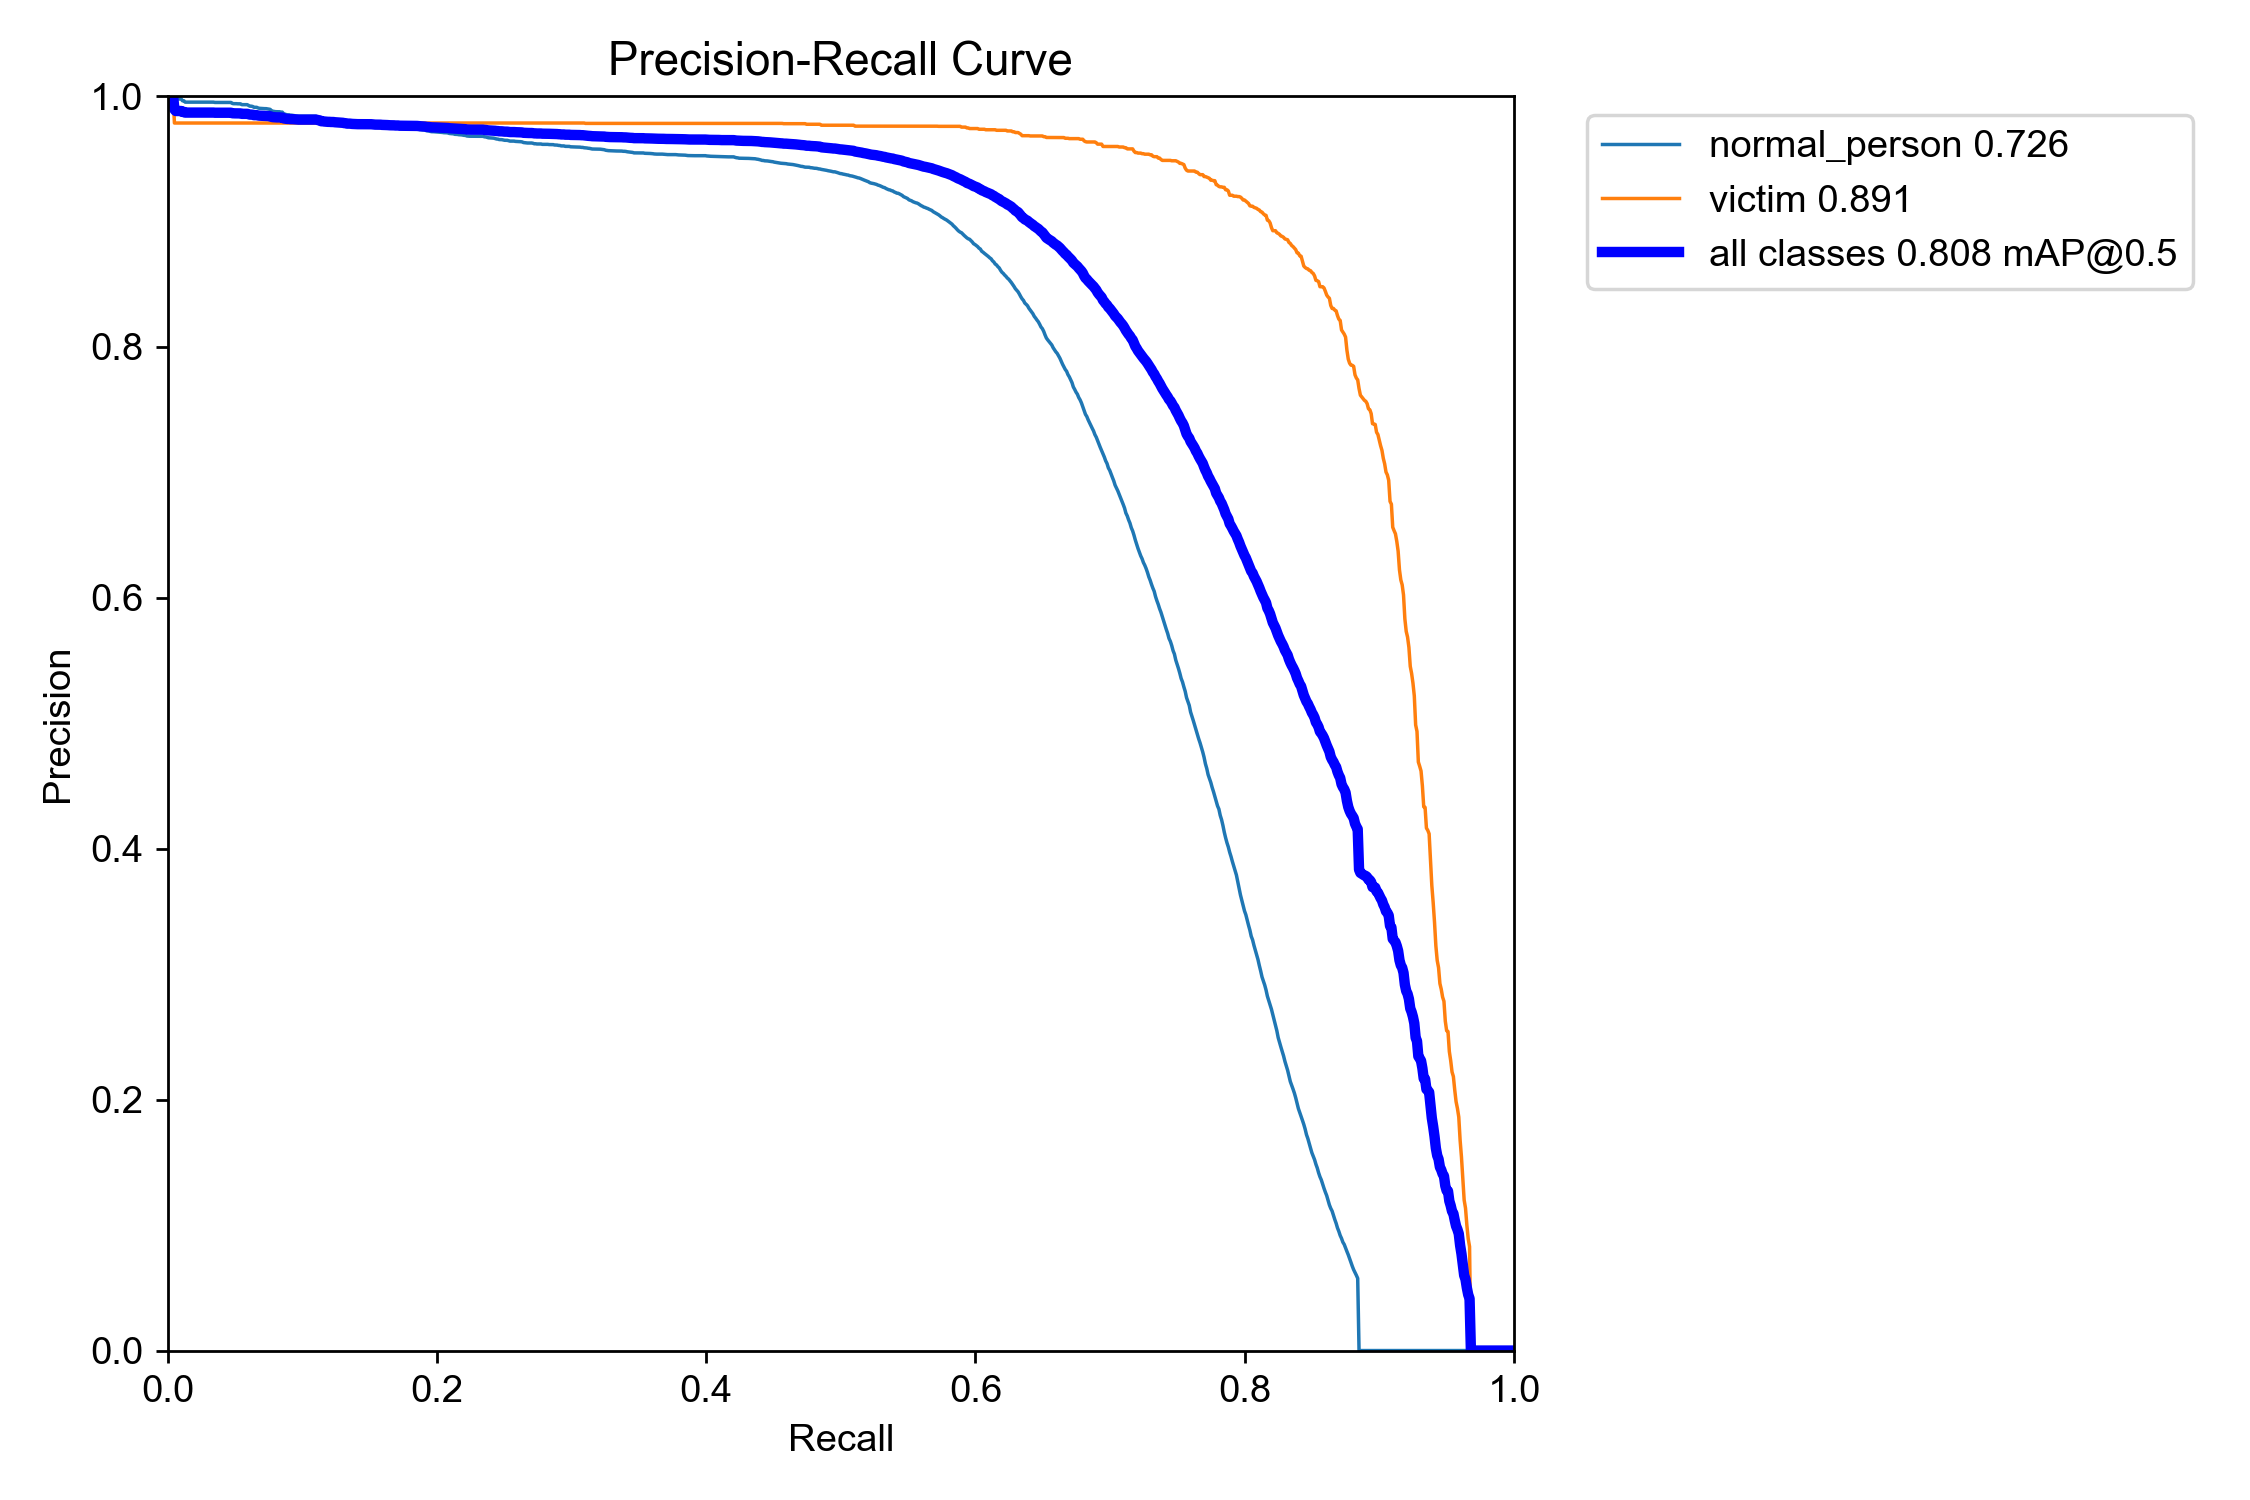
\includegraphics[width=0.65\textwidth]{Images/yolo_ai/rescue_pr_curve.png}
    \caption[Đường cong Precision-Recall của mô hình cứu hộ]{\bfseries\fontsize{12pt}{0pt}\selectfont Đường cong Precision-Recall của mô hình cứu hộ}
    \label{fig:rescue_pr_curve}
\end{figure}

Độ chính xác trung bình toàn cục mAP@0.5 đạt mức 73.8\% (0.738). Hiệu năng ghi nhận sự mất cân đối rõ rệt: lớp Victim đạt mAP@0.5 khá tốt ở mức 85.0\% (0.850), trong khi lớp Normal kéo tụt hiệu năng chung xuống mức mAP@0.5 chỉ đạt 62.7\% (0.627). Chỉ số F1 tổng hợp đạt đỉnh (0.75) khi ngưỡng tin cậy được thiết lập ở mức khá thấp là 0.359.

\paragraph{Đánh giá độ nhạy cảm qua ma trận nhầm lẫn (Confusion Matrix):}
Ma trận nhầm lẫn chuẩn hóa cung cấp cái nhìn chi tiết nhất về các lỗi nhận diện của mô hình cứu hộ, thể hiện ở Hình \ref{fig:rescue_confusion_matrix}.

\begin{figure}[H]
    \centering
    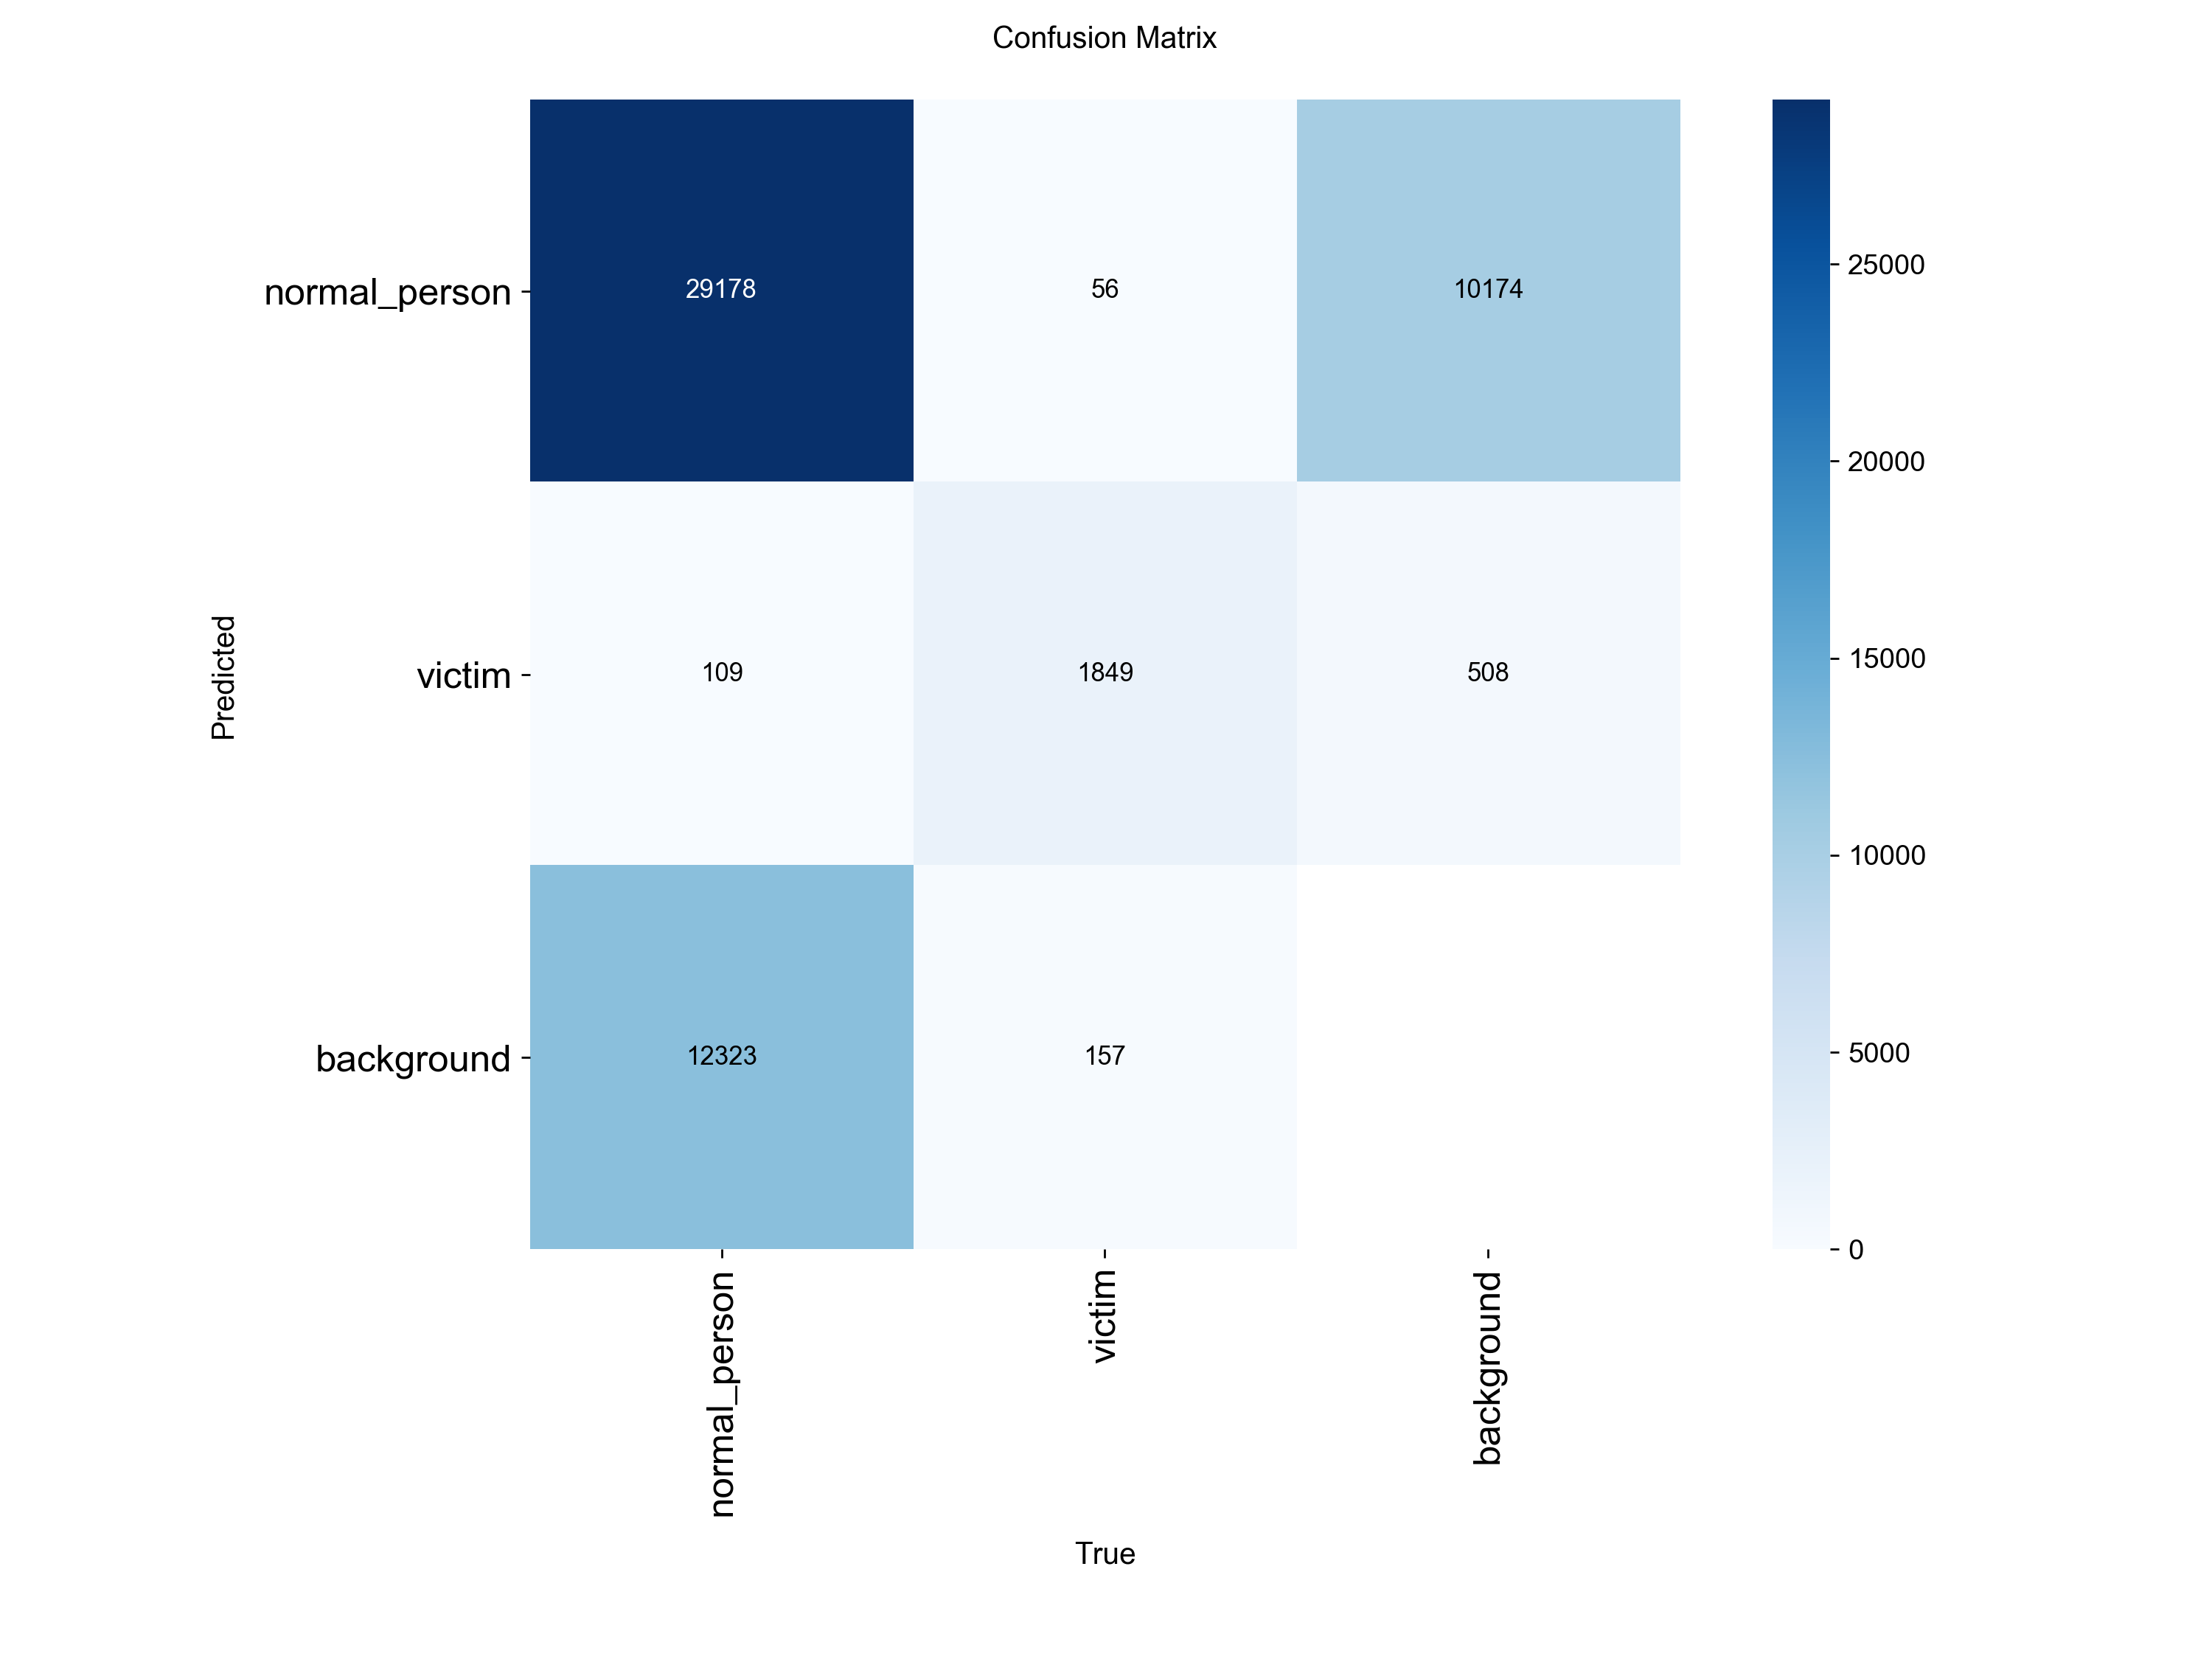
\includegraphics[width=0.6\textwidth]{Images/yolo_ai/rescue_confusion_matrix.png}
    \caption[Ma trận nhầm lẫn chuẩn hóa của mô hình nhận diện cứu hộ]{\bfseries\fontsize{12pt}{0pt}\selectfont Ma trận nhầm lẫn chuẩn hóa của mô hình nhận diện cứu hộ}
    \label{fig:rescue_confusion_matrix}
\end{figure}

Mô hình thực hiện tốt nhiệm vụ ưu tiên khi nhận diện đúng 81\% đối tượng là nạn nhân (Victim). Chỉ có 9\% bị bỏ sót thành cảnh nền và 10\% nhận nhầm thành người bình thường. Tuy nhiên, điểm yếu nằm ở lớp người bình thường (Normal) khi tỷ lệ dự đoán đúng chỉ đạt 59\% và có tới 40\% trường hợp mô hình nhận diện sai các yếu tố nhiễu của môi trường thành người Normal. 

Để khắc phục hạn chế này trong tương lai, giải pháp đề xuất là bổ sung thêm các hình ảnh cảnh nền trống (background images) không chứa người vào tập dữ liệu huấn luyện để mạng nơ-ron học cách phân biệt tốt hơn bối cảnh môi trường.


\subsection*{Kết luận Chương 2}
\addcontentsline{toc}{subsection}{Kết luận Chương 2}

Chương 2 đã trình bày toàn diện cơ sở lý thuyết và quy trình thiết kế, xây dựng hệ thống Drone cứu hộ. Về lý thuyết bay, mô hình động lực học Newton-Euler mô tả chuyển động của Quadcopter, thuật toán bộ lọc bù dung hợp IMU đạt sai số dưới $1^\circ$ cùng bộ điều khiển phản hồi PID nối tầng kép được xây dựng và tối ưu rời rạc. Về phần cứng, bo mạch Flight Controller PCB được tự thiết kế và chế tạo dựa trên STM32F103C8T6, đảm bảo chống nhiễu nguồn qua bộ lọc LC và tụ phân tầng; hệ thống nguồn điện ba cấp (3S LiPo $\rightarrow$ Buck 5V $\rightarrow$ LDO 3.3V) đảm bảo hoạt động ổn định cho tất cả module; Drone Quad-X được lắp ráp hoàn chỉnh với tỉ lệ lực đẩy/trọng lượng 3.58. Về phần mềm AI, hệ thống triển khai chiến thuật Cascade Pipeline gồm 4 mô hình YOLOv8 chuyên biệt (YOLOv8s làm nhiệm vụ gác cổng cắt ảnh, truyền tiếp cho YOLOv8s-Pose, YOLOv8s-Posture và YOLOv8s-Rescue phân tích chuyên sâu), sau đó tích hợp trong thuật toán dung hợp quyết định tính điểm Danger Score -- loại bỏ nhiễu bối cảnh và giảm thiểu đáng kể cảnh báo nhầm. Phần mềm GCS xây dựng theo kiến trúc đa luồng bất đồng bộ đảm bảo xử lý video trơn tru đồng thời ghi sự kiện cứu hộ. Các sản phẩm của chương này là cơ sở trực tiếp cho việc thực nghiệm và đánh giá tại Chương 3.
